\documentclass[11pt,a4paper]{article}
\usepackage[utf8]{inputenc}
\usepackage[T1]{fontenc}
\usepackage[margin=2.4cm]{geometry}
\usepackage{amsmath,amssymb,amsthm,bm,mathtools}
\usepackage{graphicx}
\usepackage{booktabs}
\usepackage{xcolor}
\usepackage[colorlinks=true,linkcolor=blue!50!black,urlcolor=blue!50!black,citecolor=blue!50!black]{hyperref}
\usepackage{enumitem}
\usepackage{float}
\usepackage{tcolorbox}
\usepackage{caption}
\captionsetup{font=small,labelfont=bf}
\graphicspath{{../figures/}}

\newtcolorbox{keybox}[1]{colback=blue!3,colframe=blue!45!black,title={#1},fonttitle=\bfseries,boxrule=0.6pt}
\newtcolorbox{checkbox}[1]{colback=orange!4,colframe=orange!70!black,title={#1},fonttitle=\bfseries,boxrule=0.6pt}
\newtheorem{prop}{Proposition}

\newcommand{\s}{\bm{s}}
\newcommand{\E}{\mathbb{E}}
\newcommand{\one}{\mathbf{1}}

\title{\textbf{Protein sequence generation}\\[4pt]
\large Part I: a hierarchical Potts ground truth and the statistics used to judge generative models\\
Part II: learning $J$ with a factored-attention transformer\\
Part III: a masked (absorbing-state) diffusion model\
Part IV: dynamical regimes (speciation and collapse)}
\author{Project \texttt{protein\_seq\_gen}}
\date{24 September 2026}

\begin{document}
\maketitle

\begin{abstract}
We build a fully controlled ``toy universe'' of protein sequences. Every sequence is drawn from a
Potts model, a probability distribution over amino-acid strings defined by site fields $h_i(a)$ and
pairwise couplings $J_{ij}(a,b)$. We build a tree of such models (root $\to$ 3 families $\to$ 3
subfamilies each $\to$ 2 clades each, i.e.\ 18 clades), where each child is its parent plus a random
perturbation that gets smaller as we go down the tree. We check that the models are hierarchically
different: the distance $\|J^a-J^b\|$ between two clades is fixed by how far up the tree their common
ancestor sits, and it matches a closed-form prediction to within $0.5\%$. We sample 2000 sequences per
clade with a Gibbs sampler that uses the exact site conditionals (the same objects that the
pseudo-likelihood, PLM, is built from). Then we measure what AI-generated sequences will later have
to reproduce: single-site frequencies, pair correlations, sequence identity, and a PCA projection.
Part~II builds a transformer whose attention depends only on positions
($J_{ij}(a,b)=\sum_h\mathrm{softmax}_j(Q^hK^{h\top}/\sqrt d)_{ij}V^h(a,b)$), so that the network \emph{is} a Potts
model, trained by pseudo-likelihood. It comes in two versions: one learned on all clades at once, and one
conditioned on hierarchical tags (family / subfamily / clade). The code, tests and evaluation protocol are
complete. The unconditioned model has been trained ($H=128$, \S\ref{sec:res_uncond}). It finds every true contact
and learns the \emph{ancestral} couplings, but generates the three families in the wrong proportions
(22/12/66\%), a known blind spot of pseudo-likelihood. The conditioned model ($H=128$,
\S\ref{sec:res_cond}) fixes this: a clade tag generates its own clade (18/18) and a family tag its family
(98--99\%). Its couplings resolve the family level, while subfamily and clade differences are carried mainly
by the fields. Distance metrics (Hamming, nearest neighbour, Fréchet distance in PCA space) show no memorisation
and place each generated clade between the noise floor and its sibling clade. With $H=256$ heads the couplings
are recovered better, but the samples do not improve (\S\ref{sec:res_H256}). Part~III trains a masked diffusion model
(a time-conditioned transformer that outputs the probabilities of hidden residues, trained on a bound of the full
likelihood). Without any label it generates the families and clades in the right proportions and reaches $r_C=0.992$
(true samples 0.994); per clade it matches the tag-conditioned Potts model (\S\ref{sec:md_results}).
Part~IV transposes the speciation and collapse times of Biroli, Bonnaire, de Bortoli and Mézard (2024) from Gaussian
noise to masking. Trajectories decide their family after $\approx2$ revealed residues, their subfamily after
$\approx6$ and their clade after 8--16. The exact minimiser of the loss would collapse onto a training sequence after
6.2 residues, as a parameter-free (quenched) theory predicts; the trained network never does (\S\ref{sec:dr_results}).
This document explains every step from scratch and does not skip derivations.
\end{abstract}

\tableofcontents
\newpage
\part{The ground truth}

%==========================================================================================
\section{Why a synthetic ground truth?}
%==========================================================================================
Later in this project we will train AI models (autoregressive, diffusion, \dots) to generate
protein sequences. The hard question is then: \emph{are the generated sequences good?} With real
proteins we do not know the true distribution, so we can only compare with a finite alignment.

Here we invert the situation: \textbf{we choose the true distribution ourselves.} We know exactly
which model produced each sequence, which family it belongs to, and how families relate to each
other. That lets us ask precise questions of any generative model:
\begin{itemize}[nosep]
  \item does it reproduce the site frequencies and the pair correlations of each clade?
  \item does it place generated sequences in the correct family / subfamily / clade (e.g.\ in PCA space)?
  \item when conditioned on a family, does it generate that family and not a neighbouring one?
\end{itemize}

\begin{keybox}{What this document fixes (so that we implement the same thing)}
\begin{enumerate}[nosep]
  \item The representation of a sequence (\S\ref{sec:repr}).
  \item The Potts model, its energy sign convention and its gauge (\S\ref{sec:potts}--\ref{sec:gauge}).
  \item How the hierarchical tree of models is built and how its hierarchy is checked (\S\ref{sec:tree}).
  \item How we sample (Gibbs), and its link to PLM (\S\ref{sec:gibbs}).
  \item The measured quantities: $f_i$, $f_{ij}$, $C_{ij}$, identity, PCA, and the comparison metric (\S\ref{sec:stats}).
  \item The results obtained on the ground truth, which are the reference numbers for later (\S\ref{sec:results}).
\end{enumerate}
\end{keybox}

%==========================================================================================
\section{Representing a protein sequence}\label{sec:repr}
%==========================================================================================
A protein is a chain of amino acids. There are 20 standard amino acids, each with a one-letter code.
We order them alphabetically,
\[
\mathcal{A} = (\texttt{A},\texttt{C},\texttt{D},\texttt{E},\texttt{F},\texttt{G},\texttt{H},\texttt{I},\texttt{K},\texttt{L},
\texttt{M},\texttt{N},\texttt{P},\texttt{Q},\texttt{R},\texttt{S},\texttt{T},\texttt{V},\texttt{W},\texttt{Y}),
\qquad q = |\mathcal{A}| = 20 ,
\]
and replace each letter by its index $a\in\{0,\dots,q-1\}$ (\texttt{A}$\to0$, \texttt{C}$\to1$, \dots).

A sequence of length $L$ is then a vector $\s=(s_1,\dots,s_L)$ with $s_i\in\{0,\dots,q-1\}$.
We call $i$ a \emph{site} (a position along the chain) and $a$ a \emph{state} or residue.
A set of $M$ sequences of the same length (an \emph{alignment}) is an integer matrix of size $M\times L$.
In this project $L=60$ and $q=20$ (no gap symbol for now).

\paragraph{How many sequences exist?} $q^L = 20^{60}\approx 1.2\times10^{78}$. This number matters:
anything that requires summing over all sequences is impossible, and much of what follows is about
avoiding such sums.

\paragraph{One-hot encoding.} It is often convenient to write a residue $a$ at site $i$ as a vector
of $q$ zeros with a single $1$ in position $a$: $x_{i,b}=\one[s_i=b]$, where $\one[\cdot]$ is 1 if
the condition is true and 0 otherwise. A whole sequence becomes a binary vector
$\bm{x}\in\{0,1\}^{Lq}$ with exactly $L$ ones. We use this for PCA (\S\ref{sec:pca}).

%==========================================================================================
\section{The Potts model}\label{sec:potts}
%==========================================================================================
\subsection{Definition}
A Potts model assigns to every sequence an \emph{energy}
\begin{equation}\label{eq:energy}
  \boxed{\;E(\s) = -\sum_{i=1}^{L} h_i(s_i) \;-\; \sum_{1\le i<j\le L} J_{ij}(s_i,s_j)\;}
\end{equation}
and a probability given by the Boltzmann distribution
\begin{equation}\label{eq:boltz}
  \boxed{\;P(\s) = \frac{1}{Z}\,e^{-\beta E(\s)},\qquad Z=\sum_{\s} e^{-\beta E(\s)}\;}
\end{equation}
\begin{itemize}[nosep]
  \item $h_i(a)$ is the \textbf{field}: how much residue $a$ is favoured at site $i$ \emph{on its own}.
        A site with one very large $h_i(a)$ is \emph{conserved}.
  \item $J_{ij}(a,b)$ is the \textbf{coupling}: an extra bonus (if $>0$) or penalty (if $<0$) for having
        $a$ at site $i$ \emph{and} $b$ at site $j$ at the same time. In real proteins, strong couplings
        occur mostly between residues that touch in the 3D structure: if one mutates, the other
        must \emph{co-evolve} to keep the contact working.
  \item $Z$ is the \textbf{partition function}. It just makes the probabilities sum to 1, but it is a sum
        over $q^L$ terms, so we can never compute it for $L=60$.
  \item $\beta$ is an inverse temperature. We always use $\beta=1$; it is kept in the code as a knob
        (larger $\beta$ = sharper, lower-diversity distribution).
\end{itemize}
Low energy means high probability. Because of the minus signs in \eqref{eq:energy}, large positive
$h$ and $J$ make a sequence \emph{more} likely.

\paragraph{Storage and symmetry.} We store $h$ as an $L\times q$ array and $J$ as an
$L\times L\times q\times q$ array. The pair $(i,j)$ with $i<j$ is the same physical interaction as
$(j,i)$, so we impose
\begin{equation}\label{eq:sym}
  J_{ji}(b,a) = J_{ij}(a,b), \qquad J_{ii}(\cdot,\cdot) = 0 .
\end{equation}
The energy sums over $i<j$ only, so each interaction is counted once.

\paragraph{A worked example} (it is exactly \texttt{test\_energy\_by\_hand}). Take $L=2$, $q=2$, $h_1=(0.5,-0.5)$,
$h_2=(1,0)$, $J_{12}=\begin{psmallmatrix}1&0\\0&2\end{psmallmatrix}$. Then
\begin{align*}
E(0,0) &= -(0.5+1+1) = -2.5, & E(0,1) &= -(0.5+0+0) = -0.5,\\
E(1,0) &= -(-0.5+1+0) = -0.5, & E(1,1) &= -(-0.5+0+2) = -1.5,
\end{align*}
so $P \propto (e^{2.5},e^{0.5},e^{0.5},e^{1.5})$: the state $(0,0)$ is the most likely.

\subsection{Where the Potts form comes from: maximum entropy}\label{sec:maxent}
Why this particular formula? Suppose all we know about a protein family are its single-site
frequencies $f_i(a)$ and pair frequencies $f_{ij}(a,b)$ (defined precisely in \S\ref{sec:stats}).
Among all distributions $P$ that reproduce them, we pick the one that assumes nothing more: the one
with maximal entropy $S[P]=-\sum_{\s}P(\s)\log P(\s)$. This is a constrained optimisation, and we
solve it with Lagrange multipliers: $\lambda$ for normalisation, $h_i(a)$ for each single-site
constraint, $J_{ij}(a,b)$ for each pair constraint:
\begin{align*}
\mathcal{L}[P] = &-\sum_{\s}P(\s)\log P(\s) + \lambda\Big(\sum_{\s}P(\s)-1\Big)
 + \sum_{i,a}h_i(a)\Big(\sum_{\s}P(\s)\one[s_i=a]-f_i(a)\Big)\\
 &+ \sum_{i<j}\sum_{a,b}J_{ij}(a,b)\Big(\sum_{\s}P(\s)\one[s_i=a]\one[s_j=b]-f_{ij}(a,b)\Big).
\end{align*}
Take the derivative with respect to the single number $P(\s)$ for one fixed sequence $\s$. In the
sums, $\sum_a h_i(a)\one[s_i=a]$ just picks $h_i(s_i)$, and similarly for $J$:
\begin{gather*}
\frac{\partial\mathcal{L}}{\partial P(\s)} = -\log P(\s) - 1 + \lambda + \sum_i h_i(s_i) + \sum_{i<j}J_{ij}(s_i,s_j) = 0\\
\Longrightarrow\quad
P(\s) = e^{\lambda-1}\exp\Big(\sum_i h_i(s_i)+\sum_{i<j}J_{ij}(s_i,s_j)\Big).
\end{gather*}
This is exactly \eqref{eq:boltz} with $\beta=1$ and $e^{\lambda-1}=1/Z$. So \textbf{the Potts model is
the least-biased distribution consistent with one- and two-site statistics}, and $h$, $J$ are the
Lagrange multipliers of those constraints. This is why, in the rest of the project, $f_i$ and
$C_{ij}$ are \emph{the} natural statistics to check.

\subsection{Number of parameters}
$h$ has $Lq=1200$ entries. $J$ has $\binom{L}{2}q^2 = 1770\times400 = 708{,}000$ entries if every
pair is coupled. In our ground truth only pairs in a sparse \emph{contact map} are coupled
(\S\ref{sec:contacts}): 179 pairs, i.e.\ $179\times 400=71{,}600$ non-zero coupling entries.

%==========================================================================================
\section{Gauge invariance and the zero-sum gauge}\label{sec:gauge}
%==========================================================================================
\subsection{The problem: different parameters, same distribution}
Several different $(h,J)$ give exactly the same $P(\s)$. Take any numbers $u_{ij}(a)$ (one
vector per ordered pair $i\neq j$) and change
\begin{equation}\label{eq:gaugetr}
J'_{ij}(a,b) = J_{ij}(a,b) + u_{ij}(a) + u_{ji}(b),\qquad
h'_i(a) = h_i(a) - \sum_{j\neq i}u_{ij}(a) + c_i .
\end{equation}
The coupling part of the energy changes by
$-\sum_{i<j}\big[u_{ij}(s_i)+u_{ji}(s_j)\big] = -\sum_i\sum_{j\neq i}u_{ij}(s_i)$
(each ordered pair appears exactly once), and the field part changes by exactly the opposite
amount, plus the constant $-\sum_i c_i$. So $E'(\s)=E(\s)+\text{const}$ for all $\s$, and the constant
cancels in $P=e^{-E}/Z$. \textbf{The distribution is unchanged.} Such a transformation is called a
\emph{gauge transformation}.

The consequence for us: we cannot compare two models by comparing their raw $J$ arrays. Two
identical distributions could have a large $\|J-J'\|$. We must first put every model in the same,
well-defined gauge.

\subsection{The zero-sum gauge}
Notation: a dot means an average over that index,
$J_{ij}(a,\cdot)=\frac1q\sum_b J_{ij}(a,b)$, $J_{ij}(\cdot,b)=\frac1q\sum_a J_{ij}(a,b)$,
$J_{ij}(\cdot,\cdot)=\frac1{q^2}\sum_{a,b}J_{ij}(a,b)$.
Every $q\times q$ block can be split exactly into four pieces:
\[
J_{ij}(a,b) = \underbrace{J_{ij}(\cdot,\cdot)}_{\text{constant}}
 + \underbrace{\big[J_{ij}(a,\cdot)-J_{ij}(\cdot,\cdot)\big]}_{\text{function of $a$ only}}
 + \underbrace{\big[J_{ij}(\cdot,b)-J_{ij}(\cdot,\cdot)\big]}_{\text{function of $b$ only}}
 + J^0_{ij}(a,b),
\]
\begin{equation}\label{eq:J0}
\boxed{\;J^0_{ij}(a,b) = J_{ij}(a,b) - J_{ij}(a,\cdot) - J_{ij}(\cdot,b) + J_{ij}(\cdot,\cdot)\;}
\end{equation}
(add the four terms to check that they give back $J_{ij}(a,b)$). The ``function of $a$ only'' and
``function of $b$ only'' pieces are exactly of the gauge form \eqref{eq:gaugetr}, so they can be
moved into the fields. Summing the $a$-only pieces from all partners $j$ of site $i$
(using the symmetry \eqref{eq:sym}, the $b$-only piece of $J_{ji}$ is the $a$-only piece of $J_{ij}$) gives
\begin{equation}\label{eq:h0}
\boxed{\;\tilde h_i(a) = h_i(a) + \sum_{j\neq i} J_{ij}(a,\cdot),\qquad h^0_i(a) = \tilde h_i(a) - \tilde h_i(\cdot)\;}
\end{equation}
where the last step removes a constant per site. By construction $\sum_a J^0_{ij}(a,b)=\sum_b
J^0_{ij}(a,b)=0$ and $\sum_a h^0_i(a)=0$, which is where the name comes from. The code is
\texttt{Potts.zero\_sum\_gauge()}. \texttt{test\_zero\_sum\_gauge\_preserves\_distribution}
checks, by enumerating all $3^4$ sequences of a random model, that energies shift by one constant.

\begin{prop}[The zero-sum gauge has the smallest $\|J\|$]
Among all gauge-equivalent couplings, $J^0$ has the smallest Frobenius norm.
\end{prop}
\begin{proof}
Any gauge-equivalent block is $J^0_{ij}(a,b)+g(a)+k(b)$ for some vectors $g,k$ (constants included).
Its squared norm is
\begin{align*}
\sum_{a,b}\big(J^0+g+k\big)^2 &= \sum_{a,b}(J^0)^2 + \sum_{a,b}(g+k)^2\\
 &\quad + 2\sum_a g(a)\underbrace{\sum_bJ^0(a,b)}_{=0} + 2\sum_b k(b)\underbrace{\sum_aJ^0(a,b)}_{=0}\\
 &\ge\;\sum_{a,b}(J^0)^2 .\qedhere
\end{align*}
\end{proof}
Geometrically, \eqref{eq:J0} is the \emph{orthogonal projection} of the block onto the subspace of
matrices whose rows and columns sum to zero. That subspace has dimension $(q-1)^2$: rows and columns
each lose one degree of freedom. We use this in \S\ref{sec:theory}.

\begin{keybox}{Convention used everywhere}
All stored ground-truth models are in the zero-sum gauge, and every distance is computed after
projecting to that gauge: $d_J(a,b)=\big\|J^{0,a}-J^{0,b}\big\|_F$ over pairs $i<j$, and
$d_h(a,b)=\|h^{0,a}-h^{0,b}\|_F$. Any model learned later must be gauge-fixed the same way before
its parameters are compared with the ground truth.
\end{keybox}

%==========================================================================================
\section{The hierarchical tree of Potts models}\label{sec:tree}
%==========================================================================================
\subsection{The contact map}\label{sec:contacts}
Real couplings are sparse: they concentrate on residue pairs in contact in the folded structure.
We mimic this with a fixed, symmetric boolean contact map $\mathcal{C}$ ($L\times L$) made of
\begin{itemize}[nosep]
  \item the backbone neighbours $(i,i+1)$: 59 pairs;
  \item 120 random ``long-range'' pairs with $|i-j|\ge 4$ (like contacts between helices or strands).
\end{itemize}
Total: $n_c=179$ pairs, 6 contacts per site on average (Figure~\ref{fig:contacts}). $J_{ij}\neq0$ only if
$(i,j)\in\mathcal{C}$. \textbf{All models in the tree share the same contact map}, as members of one
protein superfamily share a fold.

\subsection{Drawing the tree}
Write $\theta=(h,J)$. The tree has four levels, $\ell=0$ (root), $1$ (family), $2$ (subfamily),
$3$ (clade), and each level $\ell$ has its own noise scales $\sigma_h^{(\ell)}$, $\sigma_J^{(\ell)}$:
\begin{align}
\text{root:}\quad & h_i(a)\sim\mathcal{N}\big(0,(\sigma_h^{(0)})^2\big),\qquad
    J_{ij}(a,b)\sim\mathcal{N}\big(0,(\sigma_J^{(0)})^2\big)\ \text{for }(i,j)\in\mathcal{C},\ i<j,\\
\text{child at level }\ell:\quad & \theta_{\text{child}} = \theta_{\text{parent}} + \delta^{(\ell)},\qquad
  \delta^{(\ell)}\ \text{drawn like the root but with } \sigma_h^{(\ell)},\,\sigma_J^{(\ell)} .
\end{align}
All draws are independent. $J_{ji}$ is then filled by the symmetry \eqref{eq:sym}. Finally every node is
projected to the zero-sum gauge (this does not change any distribution). The parameters used:

\begin{center}
\begin{tabular}{lcccc}
\toprule
level $\ell$ & 0 root & 1 family & 2 subfamily & 3 clade\\
\midrule
number of nodes & 1 & 3 & $3\times3=9$ & $9\times2=18$\\
$\sigma_h^{(\ell)}$ & 1.5 & 0.9 & 0.5 & 0.3\\
$\sigma_J^{(\ell)}$ & 0.8 & 0.45 & 0.27 & 0.15\\
\bottomrule
\end{tabular}
\end{center}
Nodes are named \texttt{F0}, \texttt{F0.S1}, \texttt{F0.S1.C0}, \dots\ The 18 clades are the models we
sample from. The noise shrinks by a factor of about 0.55--0.6 per level, so a clade is closest to its
sibling clade, then to its cousins in the same family, then to the other families. The scales were
chosen (see \S\ref{sec:tuning}) so that the sequences look reasonably protein-like.

\subsection{Expected distances: a prediction we can test}\label{sec:theory}
Take two clades $a$ and $b$ whose lowest common ancestor (LCA) is at level $\lambda$
($\lambda=0$: different families; $1$: same family, different subfamilies; $2$: same subfamily).
Going down from the LCA, each accumulates its own independent perturbations:
\[
\theta^a-\theta^b = \sum_{\ell>\lambda}\big(\delta^{(\ell),a}-\delta^{(\ell),b}\big).
\]
The gauge projection is linear, so the gauge-fixed difference is the projection of this sum.

\paragraph{Couplings.} Consider one contact block. It is a $q\times q$ matrix $X$ of independent
$\mathcal{N}(0,\sigma^2)$ entries, and it is projected by an orthogonal projector $\Pi$ of rank $(q-1)^2$. For
such a projector, $\E\|\Pi X\|^2 = \sigma^2\,\mathrm{tr}\,\Pi = \sigma^2(q-1)^2$. (Proof: in an orthonormal
basis adapted to $\Pi$, $\Pi X$ keeps $(q-1)^2$ independent Gaussian coordinates of variance $\sigma^2$.)
The two branches are independent, so their variances add; that gives the factor 2. Summing over the
$n_c$ contact blocks and the levels below the LCA:
\begin{equation}\label{eq:dJ}
\boxed{\;\E\,d_J^2 = 2\,n_c\,(q-1)^2\sum_{\ell>\lambda}\big(\sigma_J^{(\ell)}\big)^2\;}
\end{equation}

\paragraph{Fields.} By \eqref{eq:h0}, the gauge-fixed field at site $i$ receives the raw field
perturbation (variance $\sigma_h^2$ per entry) \emph{plus} the row means $J_{ij}(a,\cdot)$ of its
$d_i$ coupling blocks. Each row mean is an average of $q$ independent Gaussians, so its variance is
$\sigma_J^2/q$. Centring over $a$ multiplies the total variance of the $q$ entries by $(q-1)/q$. Hence
$\E\|\Delta h^0_i\|^2 = (q-1)\big(\sigma_h^2 + d_i\sigma_J^2/q\big)$ per branch and level. Using
$\sum_i d_i = 2n_c$:
\begin{equation}\label{eq:dh}
\boxed{\;\E\,d_h^2 = 2\,(q-1)\sum_{\ell>\lambda}\Big(L\big(\sigma_h^{(\ell)}\big)^2 + \frac{2n_c}{q}\big(\sigma_J^{(\ell)}\big)^2\Big)\;}
\end{equation}

\paragraph{Why the hierarchy is strict and not only true on average.} $d_J^2$ is a sum of
$n_c(q-1)^2\approx 65{,}000$ independent squared Gaussians. By the law of large numbers its relative
fluctuation is of order $1/\sqrt{65{,}000}\approx0.4\%$. The gaps between relation levels are
$\approx50\%$, so every same-subfamily pair is closer than every same-family pair, which is closer
than every different-family pair. The test \texttt{test\_distances\_are\_hierarchical} asserts exactly
this strict ordering, and \texttt{test\_distances\_match\_theory} checks \eqref{eq:dJ}--\eqref{eq:dh}.

%==========================================================================================
\section{Sampling: the Gibbs sampler (and its relation to PLM)}\label{sec:gibbs}
%==========================================================================================
\subsection{The site conditional}
We cannot draw from \eqref{eq:boltz} directly, because we cannot even compute $Z$. But the probability
of the residue at \emph{one} site, given all the others, is easy. Write $\s_{-i}$ for all sites except $i$:
\[
P(s_i=a\mid\s_{-i}) = \frac{P(s_1,\dots,a,\dots,s_L)}{\sum_{b}P(s_1,\dots,b,\dots,s_L)}.
\]
$Z$ appears in the numerator and in the denominator and cancels. In the energy, every term that does
not involve site $i$ is the same in numerator and denominator and also cancels. What remains is
\begin{equation}\label{eq:cond}
\boxed{\;P(s_i=a\mid\s_{-i}) = \frac{e^{\beta H_i(a\mid\s_{-i})}}{\sum_{b=0}^{q-1} e^{\beta H_i(b\mid\s_{-i})}},\qquad
H_i(a\mid\s_{-i}) = h_i(a)+\sum_{j\neq i}J_{ij}(a,s_j)\;}
\end{equation}
This is a softmax over only $q=20$ numbers. $H_i$ is the \emph{local field}: the total ``pull'' on site
$i$ towards each residue, given its current neighbours. Because $J_{ij}=0$ outside contacts, the sum
only runs over the $\sim6$ contacts of $i$ (the code finds them automatically with
\texttt{Potts.neighbors()}).

\subsection{Link with the pseudo-likelihood (PLM)}
The pseudo-likelihood of an alignment is the product of these exact site conditionals,
$\mathrm{PL}(h,J)=\prod_{m}\prod_i P(s^m_i\mid\s^m_{-i})$. PLM \emph{infers} $(h,J)$ from data by
maximising it instead of the true likelihood, which needs $Z$. The approximation in PLM lies in
using PL as the objective for learning. The conditionals themselves are exact.

\begin{checkbox}{How ``sampling with PLM'' is implemented --- please confirm}
We read ``sample using the PLM approximation'' as: \emph{sample using the site conditionals
\eqref{eq:cond}, the building blocks of the pseudo-likelihood}. Repeatedly redrawing each site from
its conditional is the Gibbs sampler. It involves no approximation: its samples converge to the exact
Potts distribution \eqref{eq:boltz}, which we verify numerically against exact enumeration
(\S\ref{sec:gibbstests}). If instead you meant \emph{inferring} a Potts model from sequences by PLM
(e.g.\ to check that $J$ is recoverable, or as a baseline generative model), that is a separate
function we can build next.
\end{checkbox}

\subsection{The algorithm}
\begin{enumerate}[nosep]
  \item Start $M$ independent chains from uniformly random sequences.
  \item One \textbf{sweep}: for $i=1,\dots,L$, compute $H_i(\cdot\mid\s_{-i})$ for every chain and
        redraw $s_i$ from \eqref{eq:cond}.
  \item Repeat for $T_{\text{burn}}=200$ sweeps (\emph{burn-in}), then keep the final sequence of each chain.
\end{enumerate}
Since each chain gives exactly one sequence and chains never interact, the $M=2000$ sequences of a
clade are \textbf{independent} draws. All chains are updated simultaneously with vectorised numpy
(\texttt{psg.sampling.gibbs\_sample}). The categorical draw uses the inverse CDF: draw
$u\sim\mathcal{U}(0,1)$ and take the first $a$ with $\sum_{b\le a}p_b\ge u$.

\subsection{Why it works: stationarity}
\begin{prop}
If $\s\sim P$ and we redraw site $i$ from $P(\cdot\mid\s_{-i})$, the new sequence $\s'$ is still distributed as $P$.
\end{prop}
\begin{proof}
$\s'$ has $\s'_{-i}=\s_{-i}$ and a new $s'_i$. Its probability is
$\sum_{s_i}P(s_i,\s_{-i})\,P(s'_i\mid\s_{-i}) = P(\s_{-i})\,P(s'_i\mid\s_{-i}) = P(s'_i,\s_{-i}) = P(\s')$.
\end{proof}
So $P$ is a fixed point of every update, and hence of a sweep. Moreover every conditional
probability is strictly positive (it is an exponential), so in one sweep any sequence can reach any
other sequence with non-zero probability. A finite Markov chain with this property has a unique
stationary distribution and converges to it from any start (Perron--Frobenius theorem). Hence, after
enough sweeps, each chain's state is a sample of $P$.

\paragraph{How many sweeps is ``enough''?} We monitor two things. (i) The mean energy over chains
decreases from its random-start value and must reach a plateau. (ii) The energy autocorrelation
$\rho(k)=\langle\delta E_t\,\delta E_{t+k}\rangle/\langle\delta E^2\rangle$ tells how many sweeps a chain needs
to forget its past. In our models $\rho$ drops below $0.05$ within about 10--20 sweeps, so 200 sweeps
of burn-in is ten or more correlation times.

\subsection{Tests of the sampler}\label{sec:gibbstests}
\begin{itemize}[nosep]
  \item \textbf{No couplings} ($J=0$): sites are independent and $P(s_i=a)=\mathrm{softmax}(h_i)(a)$
        exactly. Measured frequencies agree to within binomial noise (Figure~\ref{fig:gibbstests}, left).
  \item \textbf{Exact enumeration}: for a coupled $L=3,q=3$ model, the $27$ probabilities are computed
        exactly and compared with 50{,}000 Gibbs samples. Total variation distance
        $\frac12\sum_{\s}|P_{\text{Gibbs}}(\s)-P(\s)| = 0.0065$ (Figure~\ref{fig:gibbstests}, right).
  \item \textbf{Conditionals}: \eqref{eq:cond} computed by the code equals ratios of exactly enumerated
        probabilities, to $10^{-10}$.
\end{itemize}
\begin{figure}[H]
\centering
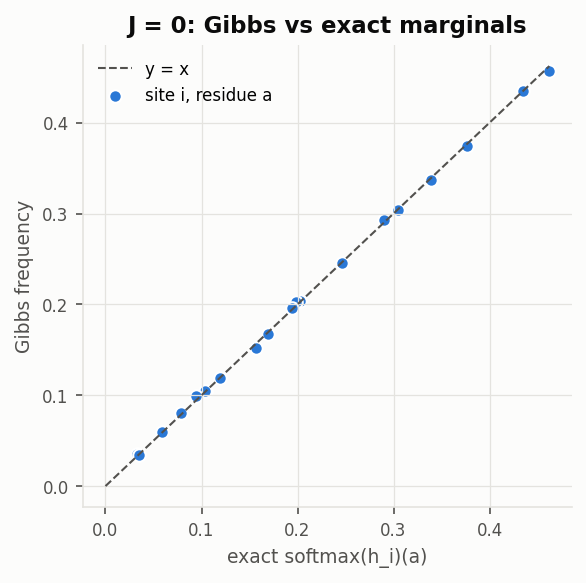
\includegraphics[width=0.36\linewidth]{tests/test_02_sampling/test_independent_sites/marginals_vs_exact.png}\hfill
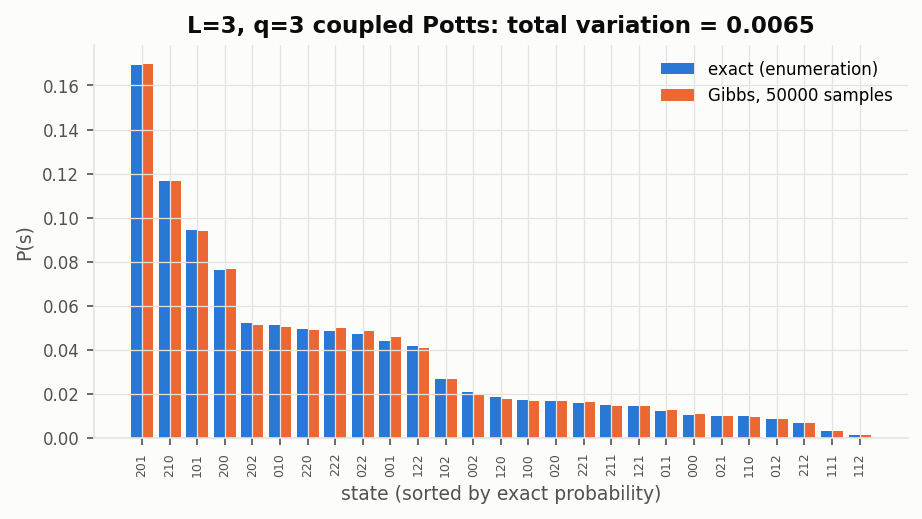
\includegraphics[width=0.6\linewidth]{tests/test_02_sampling/test_gibbs_matches_exact_distribution/state_distribution.png}
\caption{Sampler validation. Left: with $J=0$, Gibbs marginals vs.\ the exact softmax of the fields.
Right: all 27 states of a coupled $L=3,q=3$ model, exact vs.\ Gibbs.}
\label{fig:gibbstests}
\end{figure}

%==========================================================================================
\section{Measured quantities}\label{sec:stats}
%==========================================================================================
Everything below is computed from an alignment $\{\s^m\}_{m=1}^M$ (one clade, or generated sequences).

\subsection{Frequencies}
\begin{align}
f_i(a) &= \frac1M\sum_{m=1}^M\one[s^m_i=a] &&\text{(single-site frequency, an $L\times q$ table)}\\
f_{ij}(a,b) &= \frac1M\sum_{m=1}^M\one[s^m_i=a]\,\one[s^m_j=b] &&\text{(pair frequency)}
\end{align}
Useful identities, which follow from summing an indicator over all its values:
$\sum_a f_i(a)=1$; $\sum_b f_{ij}(a,b)=f_i(a)$ (marginalisation); $f_{ii}(a,b)=\delta_{ab}f_i(a)$.
With one-hot vectors, all pair frequencies at once are one matrix product,
$f = \frac1M X^\top X$ with $X\in\{0,1\}^{M\times Lq}$, which is how the code computes them.

\subsection{Connected correlations}
\begin{equation}\label{eq:C}
\boxed{\;C_{ij}(a,b) = f_{ij}(a,b) - f_i(a)\,f_j(b),\qquad i\neq j\;}
\end{equation}
If sites $i$ and $j$ were independent, $f_{ij}(a,b)$ would equal $f_i(a)f_j(b)$ and $C$ would vanish.
So $C$ measures how far the pair is from independence. From the marginalisation identity,
$\sum_b C_{ij}(a,b)=f_i(a)-f_i(a)\cdot1=0$.

\emph{Worked example} (\texttt{test\_frequencies\_by\_hand}). Take the alignment $\{00,01,11,11\}$ ($q=2$):
$f_1=(\tfrac12,\tfrac12)$, $f_2=(\tfrac14,\tfrac34)$, $f_{12}(1,1)=\tfrac12$, so
$C_{12}(1,1)=\tfrac12-\tfrac12\cdot\tfrac34=0.125>0$: residue 1 at site 1 comes with residue 1 at site 2
more often than chance.

\paragraph{Correlations are not couplings.} If $i$ is coupled to $j$ and $j$ to $k$, then $i$ and $k$
become correlated \emph{through} $j$, even with $J_{ik}=0$. So $C$ is non-zero on many non-contact
pairs (Figure~\ref{fig:corr}). This is why inferring $J$ (DCA, PLM) is needed to find contacts, and it
is also why reproducing $C$ is a demanding test for a generative model: it must capture direct and
indirect effects together.

\paragraph{Finite-sample noise.} An estimated frequency has standard error
$\sqrt{f(1-f)/M}$. With $M=2000$ and typical $f_{ij}\sim10^{-2}$, that is $\sim2\times10^{-3}$, the same
order as many true $C$ values. So even two perfect samples of the same model do not have identical
$C$. We therefore always report a \textbf{noise floor} (next subsection).

\subsection{The comparison metric}\label{sec:metric}
To compare a reference alignment $R$ with a generated one $G$ (function \texttt{compare\_statistics}):
\begin{itemize}[nosep]
  \item $r_{f}$ = Pearson correlation between all $Lq$ values $f^R_i(a)$ and $f^G_i(a)$;
  \item $r_C$ = Pearson correlation between all $\binom L2q^2$ values $C^R_{ij}(a,b)$ and $C^G_{ij}(a,b)$, $i<j$;
  \item RMSE of each, and the slope of $C^G$ vs.\ $C^R$ (a slope $<1$ means correlations are too weak).
\end{itemize}
Pearson's $r=\frac{\sum_k(x_k-\bar x)(y_k-\bar y)}{\sqrt{\sum_k(x_k-\bar x)^2\sum_k(y_k-\bar y)^2}}\in[-1,1]$
is 1 when the points lie on an increasing straight line. $r_C$ is the standard score for
Potts/DCA-type generative models.

\textbf{Noise floor:} split the 2000 sequences of a clade into two random halves and compute the metric
between the halves. A perfect generator cannot do better than this (at the same sample size). A useful
sanity check that the metric can tell things apart: compare a clade with its sibling clade and with
a clade from another family. The scores must decrease in that order.

\subsection{Sequence identity}
$\mathrm{id}(\s,\s')=\frac1L\sum_i\one[s_i=s'_i]$, averaged over random pairs within a set or between
two sets. Random sequences give $1/q=5\%$.

\subsection{Principal component analysis}\label{sec:pca}
Each sequence is a one-hot vector $\bm{x}\in\{0,1\}^{Lq}$ (1200 dimensions). PCA finds the directions
along which the sequences vary most.
\begin{enumerate}[nosep]
\item Centre: $\bm\mu=\frac1M\sum_m\bm{x}^m$ (this is just $f_i(a)$ laid out as a vector), $\bar{\bm x}^m=\bm x^m-\bm\mu$.
\item Covariance: $\Sigma=\frac1{M-1}\sum_m\bar{\bm x}^m\bar{\bm x}^{m\top}$. Its $(i,a),(j,b)$ entry is
      (up to $M/(M-1)$) $f_{ij}(a,b)-f_i(a)f_j(b)$, i.e.\ \textbf{the covariance matrix is exactly the
      connected-correlation tensor $C$} (with diagonal blocks $\mathrm{diag}(f_i)-f_if_i^\top$).
\item The variance of the data along a unit direction $\bm u$ is $\bm u^\top\Sigma\bm u$. Maximise it
      subject to $\|\bm u\|=1$ with a Lagrange multiplier:
      $\nabla_{\bm u}\big[\bm u^\top\Sigma\bm u-\lambda(\bm u^\top\bm u-1)\big]=2\Sigma\bm u-2\lambda\bm u=0$, so
      $\Sigma\bm u=\lambda\bm u$. The best direction is an eigenvector, and the variance along it is its
      eigenvalue $\lambda$. So PC1 is the top eigenvector, PC2 the next one (orthogonal to PC1), etc.
\item Projection: $z_k^m=\bm u_k^\top(\bm x^m-\bm\mu)$. Explained variance ratio of PC $k$:
      $\lambda_k/\sum_{k'}\lambda_{k'}$.
\end{enumerate}
\textbf{Important for later:} the PCA is fitted \emph{once} on all ground-truth sequences, and its
$\bm\mu$ and $\bm u_k$ are saved (\texttt{evaluations/ground\_truth/pca\_reference.npz}). Generated
sequences will be projected with the \emph{same} axes, so that they appear on the same map as the
real families.

%==========================================================================================
\section{Results on the ground truth}\label{sec:results}
%==========================================================================================
% Results section, numbers from evaluations/ground_truth/*.json (config: configs/ground_truth.json)

\subsection{Choice of the noise scales}\label{sec:tuning}
The scales $\sigma_h,\sigma_J$ set how ``protein-like'' the sequences are. Too weak, and sequences are
almost random: our first try ($\sigma_h^{(0)}=1$, $\sigma_J^{(0)}=0.5$) gave only 18\% identity
within a clade, and correlations on contacts were barely above noise. Too strong, and the model
freezes into a few sequences and Gibbs mixes slowly. We scanned four settings and kept
$\sigma^{(0)}_h=1.5$, $\sigma^{(0)}_J=0.8$. With these, the mean site entropy is $\approx1.6$ nats
(the maximum, $\log 20$, is 3.0), identity is $\approx34\%$ within a clade and $\approx15\%$
between families (real families typically sit at 25--40\%), and the energy autocorrelation is gone
within 20 sweeps.

\subsection{The hierarchy of the models (on $J$ and $h$)}
\begin{figure}[H]
\centering
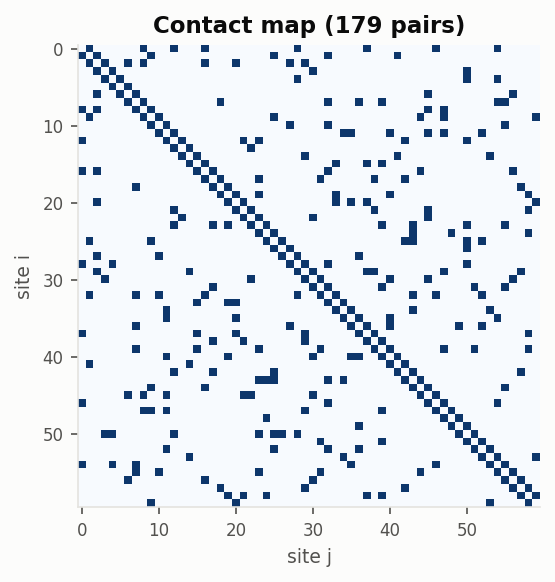
\includegraphics[width=0.3\linewidth]{ground_truth/01_hierarchy/contact_map.png}\hfill
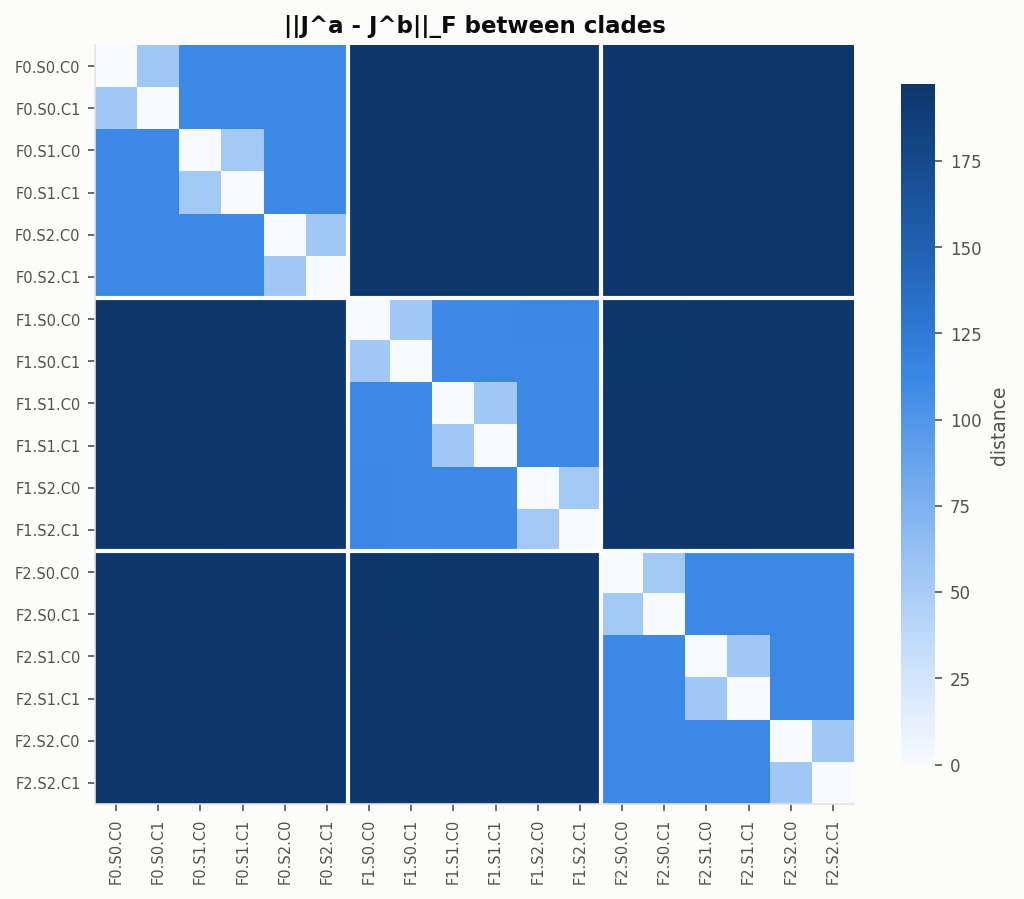
\includegraphics[width=0.66\linewidth]{ground_truth/01_hierarchy/J_distance_matrix.png}
\caption{Left: the shared contact map (59 backbone + 120 long-range pairs). Right:
$d_J=\|J^{0,a}-J^{0,b}\|_F$ between the 18 clades, ordered by family / subfamily / clade. The
nested block structure is the hierarchy.}
\label{fig:contacts}
\end{figure}

\begin{figure}[H]
\centering
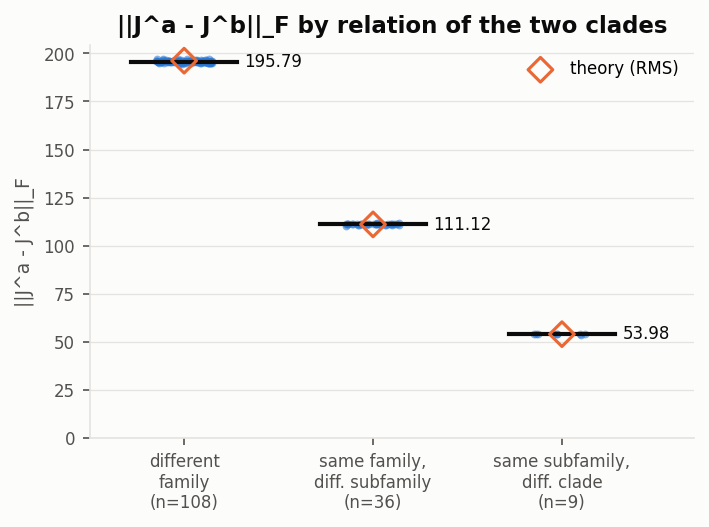
\includegraphics[width=0.49\linewidth]{ground_truth/01_hierarchy/J_distance_by_relation.png}\hfill
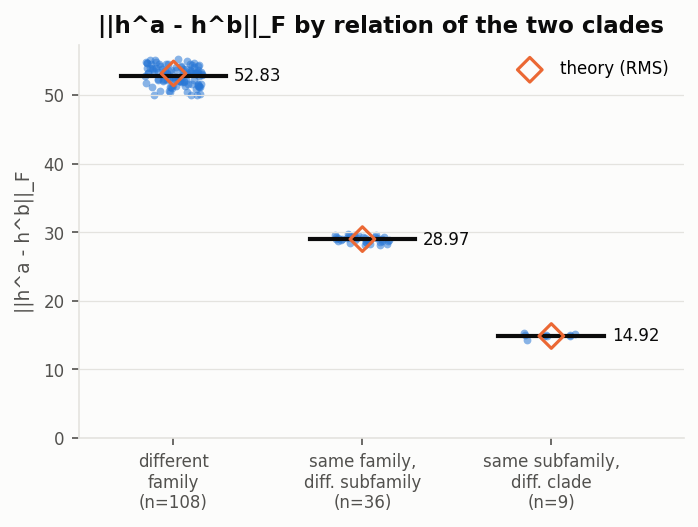
\includegraphics[width=0.49\linewidth]{ground_truth/01_hierarchy/h_distance_by_relation.png}
\caption{Distances between pairs of clades, grouped by the level of their common ancestor.
Dots are pairs, black bars their mean, orange diamonds the theoretical RMS from
\eqref{eq:dJ}--\eqref{eq:dh}.}
\label{fig:dist}
\end{figure}

\begin{center}\small
\begin{tabular}{lccccc}
\toprule
relation & pairs & $d_J$ range & $d_J$ RMS & theory \eqref{eq:dJ} & $d_h$ RMS (theory \eqref{eq:dh})\\
\midrule
different family & 108 & 194.7 -- 197.1 & 195.8 & 196.2 & 52.8 (53.2)\\
same family, diff.\ subfamily & 36 & 110.4 -- 111.7 & 111.1 & 111.0 & 29.0 (29.0)\\
same subfamily, diff.\ clade & 9 & 53.7 -- 54.2 & 54.0 & 53.9 & 14.9 (14.9)\\
\bottomrule
\end{tabular}
\end{center}
\textbf{Check passed:} the ordering is strict (the ranges do not overlap) for both $J$ and $h$, and
the measured distances agree with the closed-form prediction to within 0.5\% for $J$ and 1\% for $h$.
The models are therefore hierarchically different in exactly the designed way.

\subsection{Sampling}
18 clades $\times$ 2000 independent chains $\times$ 200 sweeps, about 33\,s per clade.
Over the last 100 sweeps, the energy autocorrelation averaged over clades is $\rho(1)=0.44$,
$\rho(5)=0.11$, $\rho(20)=-0.03$, and the mean energy drifts by less than $0.2$ (on energies of about
$-260$ to $-290$) between the third and fourth quarters of the run: the chains are at equilibrium.

\begin{figure}[H]
\centering
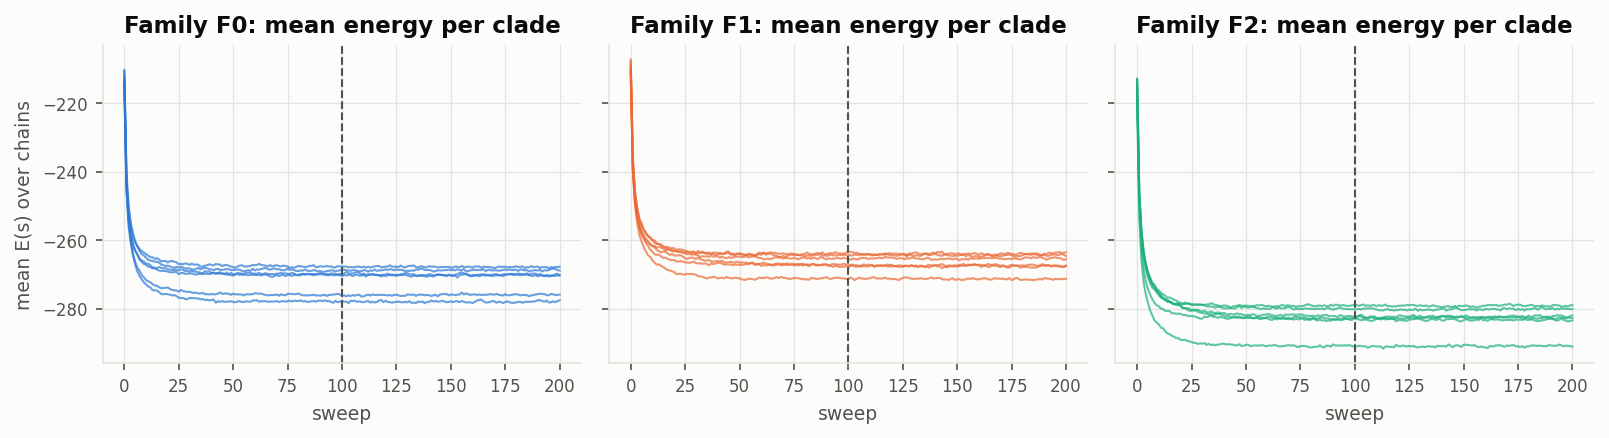
\includegraphics[width=0.95\linewidth]{ground_truth/02_sampling/energy_traces.png}
\caption{Mean energy over 2000 chains vs.\ sweep, one line per clade. The energy reaches its plateau within 20--50
sweeps; the dashed line marks the start of the window used for the diagnostics.}
\label{fig:energytraces}
\end{figure}

\subsection{PCA}
The PCA is fitted on all 36{,}000 sequences. PC1 and PC2 explain $7.2\%$ and $5.0\%$ of the variance;
the next ones about $1\text{--}2\%$ each. That low percentage is normal: the 1200-dimensional one-hot
space is dominated by site-wise noise. The two leading PCs are exactly the ``between-family''
directions (three families need two dimensions to be separated), so the three families form three
disjoint clouds (Figure~\ref{fig:pca}). Within one family (PCA fitted on that family only), the three
subfamilies separate, with some overlap. Clades, the finest level, do not separate visibly in two
dimensions. The metrics below show they are nonetheless statistically different.

\begin{figure}[H]
\centering
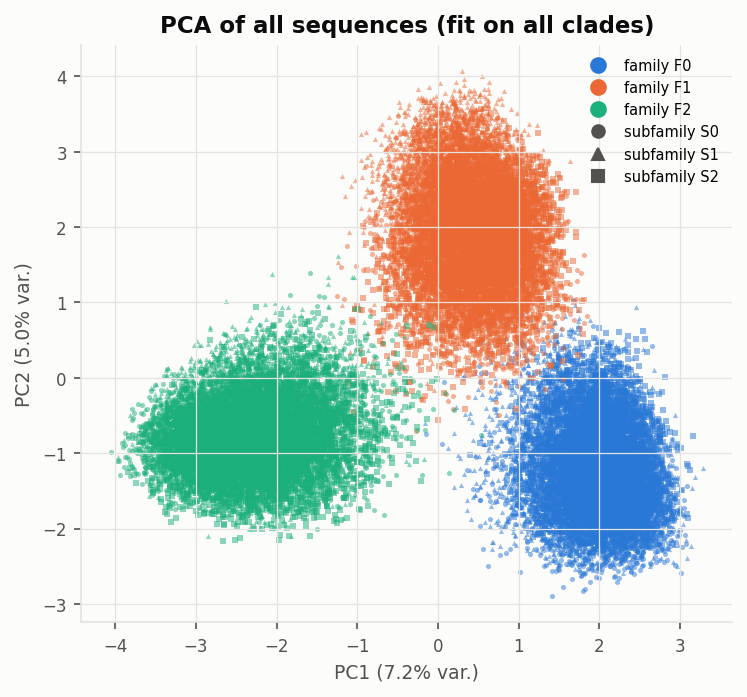
\includegraphics[width=0.55\linewidth]{ground_truth/03_analysis/pca_all_PC1_PC2.png}
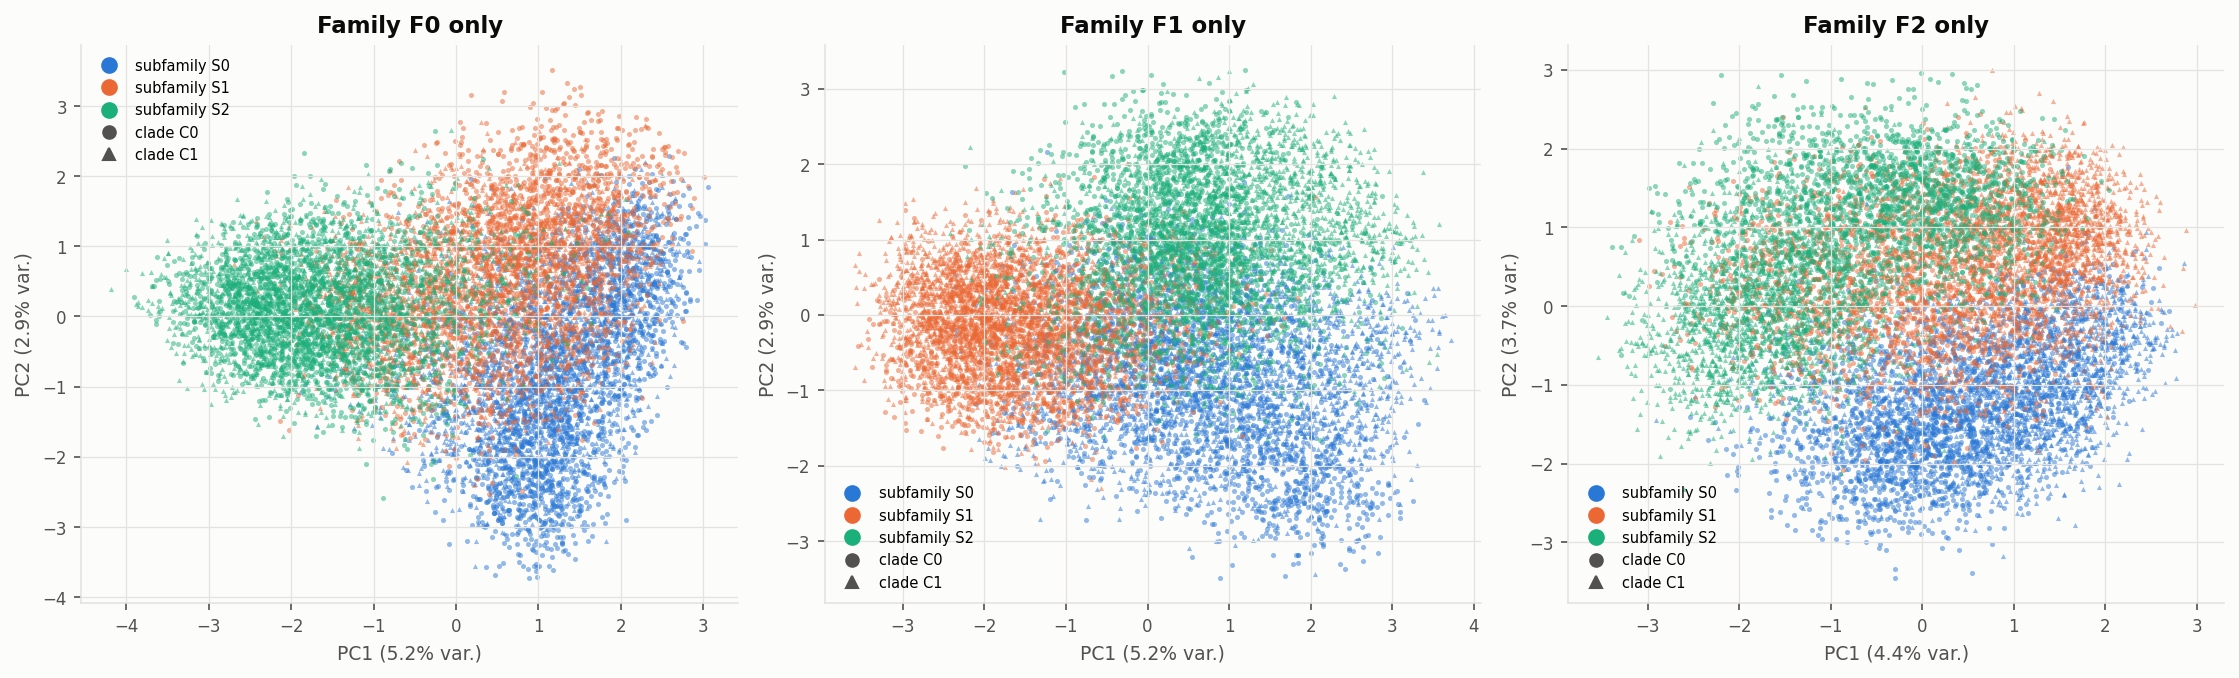
\includegraphics[width=\linewidth]{ground_truth/03_analysis/pca_within_family.png}
\caption{Top: all sequences on the reference PCA axes, colour = family, marker = subfamily. Bottom:
one PCA per family, colour = subfamily, marker = clade.}
\label{fig:pca}
\end{figure}

\subsection{Frequencies and correlations}
\begin{figure}[H]
\centering
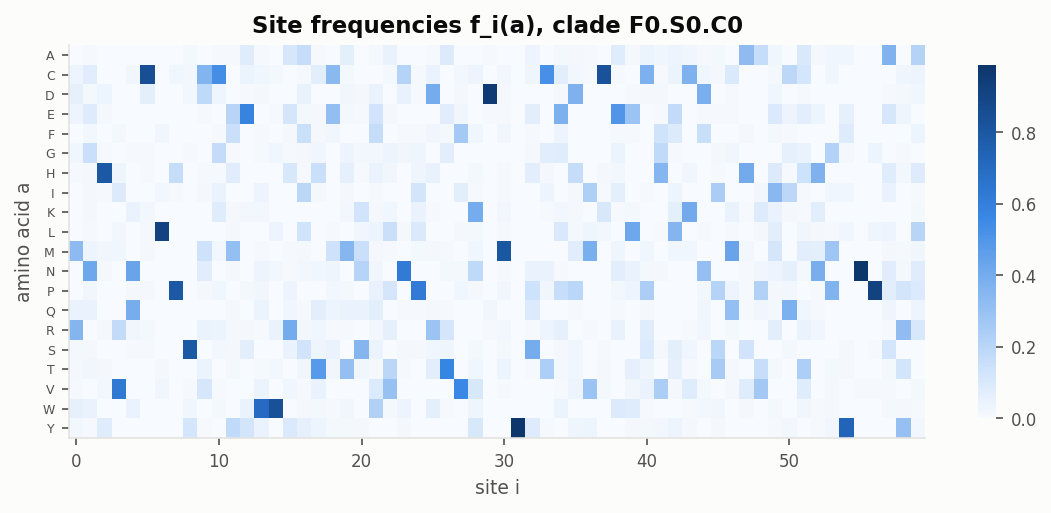
\includegraphics[width=0.52\linewidth]{ground_truth/03_analysis/site_frequencies_F0.S0.C0.png}\hfill
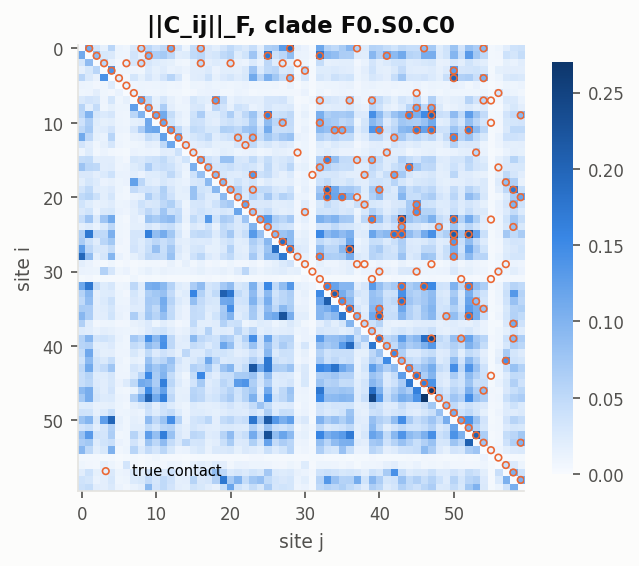
\includegraphics[width=0.44\linewidth]{ground_truth/03_analysis/correlation_strength_F0.S0.C0.png}
\caption{Clade \texttt{F0.S0.C0}. Left: $f_i(a)$; dark cells are conserved residues. Right: the
strength $\|C_{ij}\|_F$ of each pair's correlation, with true contacts circled (upper triangle).}
\label{fig:corr}
\end{figure}
The mean correlation strength is $0.100$ on contact pairs and $0.035$ on non-contacts. Contacts are
clearly enriched, but many non-contacts are correlated as well. These are the \emph{indirect}
correlations of \S\ref{sec:stats}, plus finite-sample noise. Rows that are almost blank (e.g.\ site
31) are highly conserved sites: a site that barely varies cannot co-vary with anything.

\subsection{The metric and its reference values}\label{sec:refvalues}
We compute the metric of \S\ref{sec:metric} between every pair of clades, and between two halves of
each clade (the noise floor):

\begin{center}
\begin{tabular}{lccc}
\toprule
compared sets & $r_f$ (mean) & $r_C$ (mean [min, max]) & identity\\
\midrule
same clade, two halves of 1000 (\textbf{noise floor}) & 0.998 & 0.83 [0.80, 0.88] & 0.34\\
same subfamily, different clade & 0.90 & 0.63 [0.55, 0.69] & 0.31\\
same family, different subfamily & 0.75 & 0.35 [0.25, 0.46] & 0.27\\
different family & 0.37 & 0.08 [0.04, 0.13] & 0.15\\
\bottomrule
\end{tabular}
\end{center}

\begin{figure}[H]
\centering
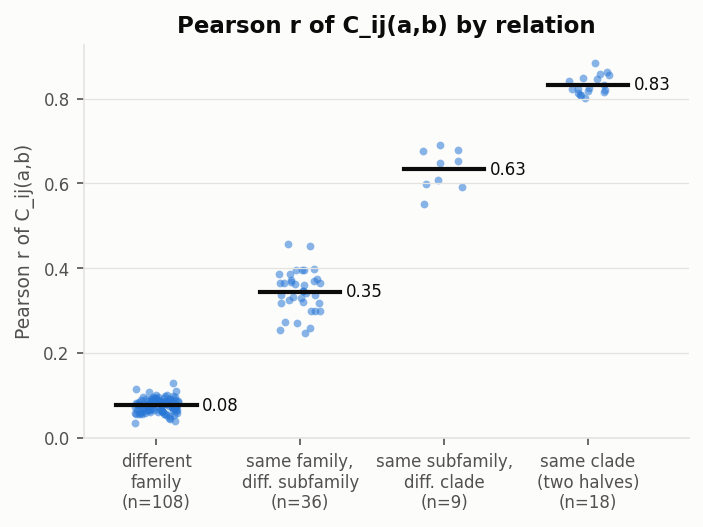
\includegraphics[width=0.49\linewidth]{ground_truth/03_analysis/pearson_C_by_relation.png}\hfill
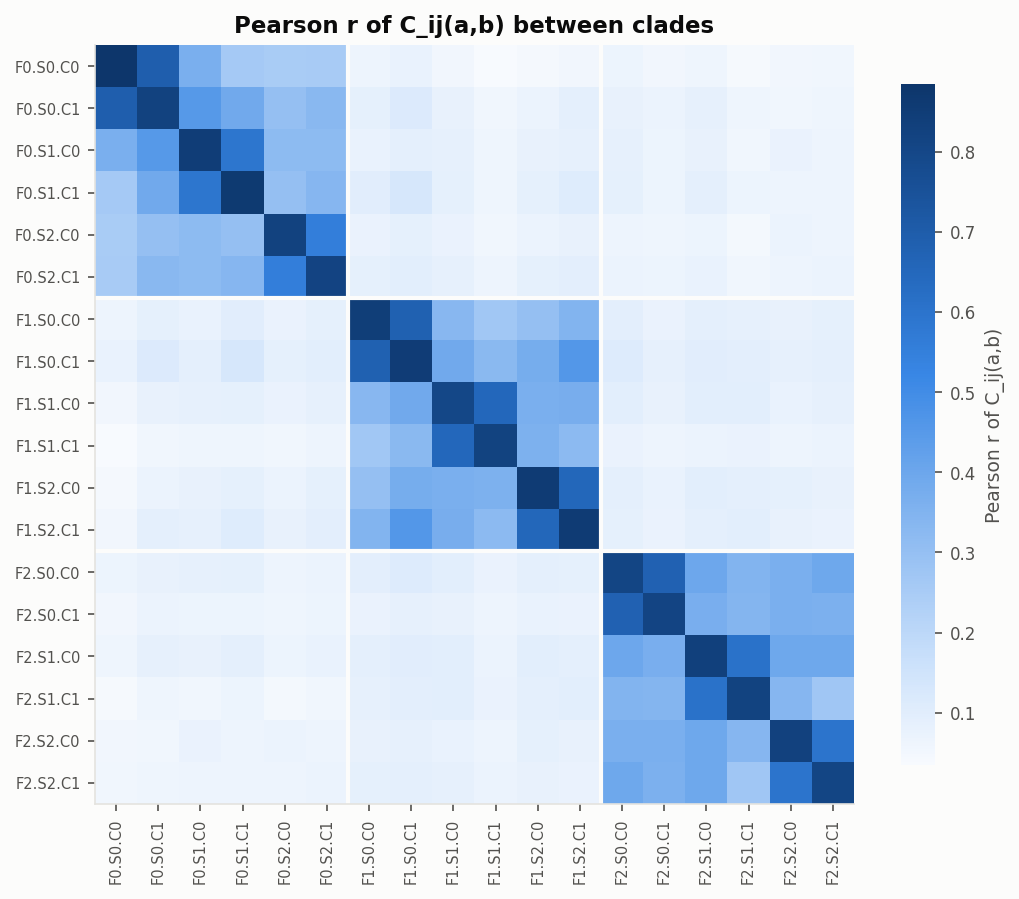
\includegraphics[width=0.49\linewidth]{ground_truth/03_analysis/pearson_C_matrix.png}
\caption{Pearson $r_C$ of the connected correlations. Left: grouped by relation. Right: all
clade pairs (the diagonal is the half-vs-half noise floor).}
\end{figure}

\begin{figure}[H]
\centering
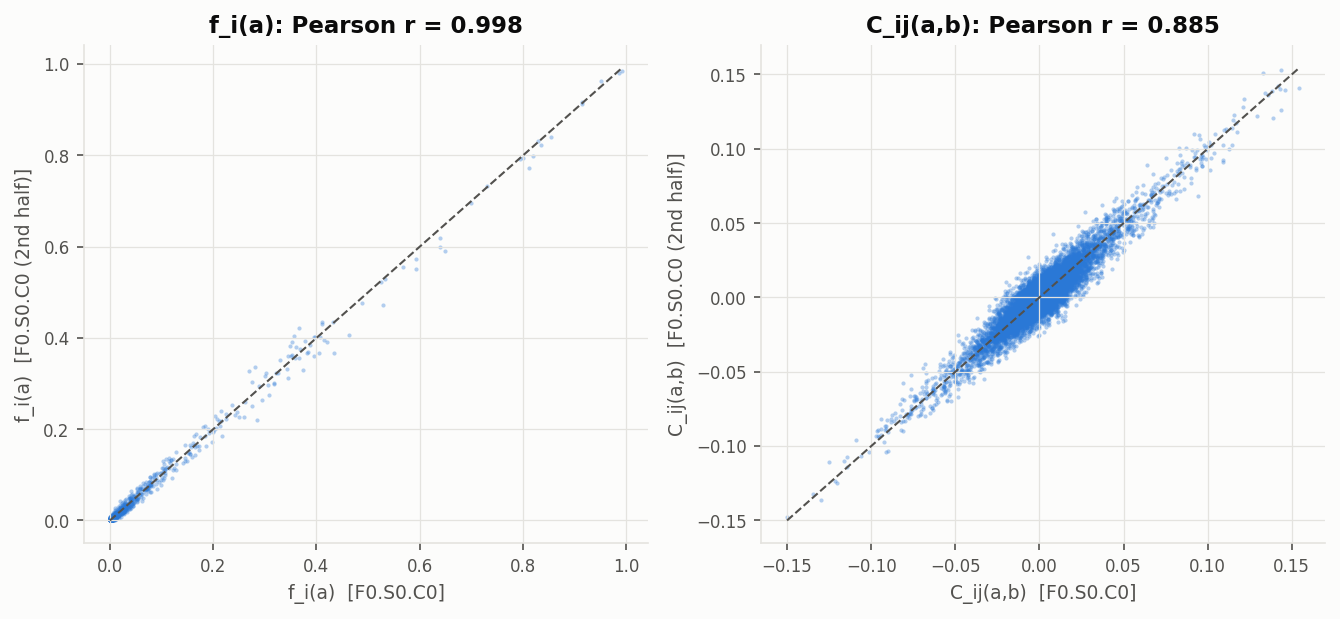
\includegraphics[width=0.49\linewidth]{ground_truth/03_analysis/compare_same_clade_halves.png}\hfill
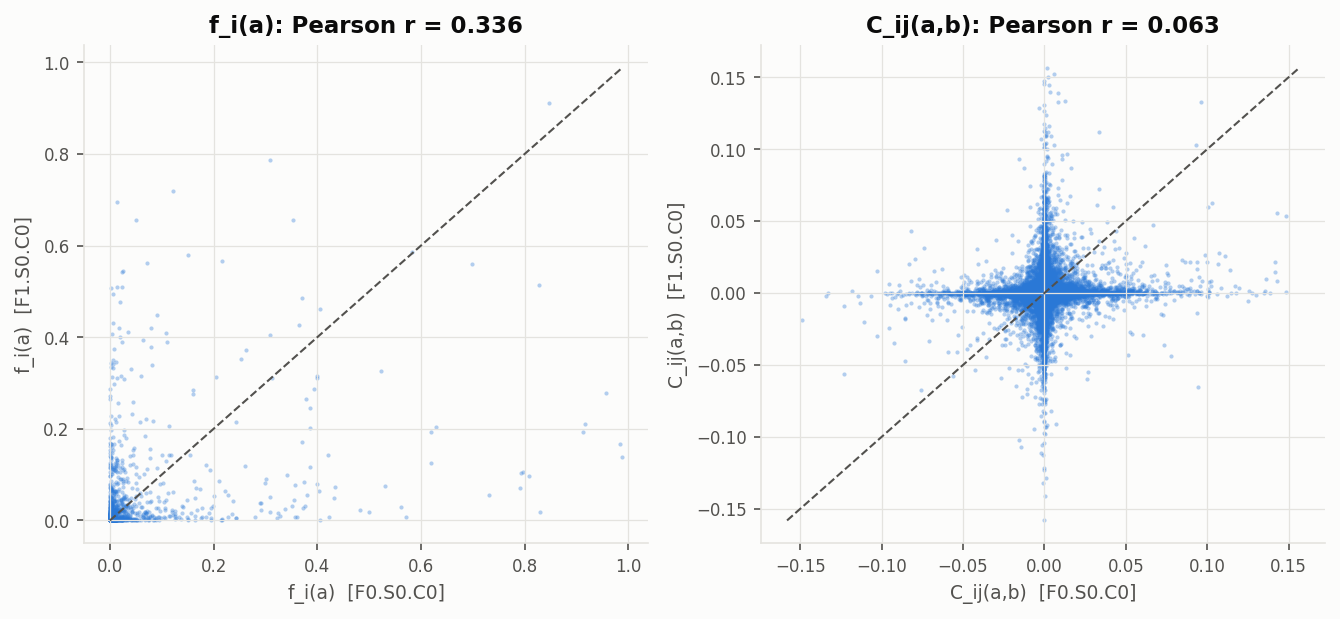
\includegraphics[width=0.49\linewidth]{ground_truth/03_analysis/compare_other_family.png}
\caption{Scatter of statistics. Left: two halves of the same clade (the best achievable). Right:
the same clade vs.\ a clade of another family (what a generator that got the family wrong would
score).}
\end{figure}

\begin{keybox}{How to read a future generative model's score}
For a model asked to generate clade $X$, compute $r_C$ against the held-out ground-truth sequences of
$X$ at matching sample size. Values near $0.83$ mean it reproduces the clade as well as fresh
ground-truth samples would. About $0.63$ means it only captured the subfamily, about $0.35$ only the
family, and below $0.1$ it is not even the right family. Note that $r_C$ depends on sample size
(noise), so compare at the same $M$.
\end{keybox}


% ==========================================================================================
% PART II : learning J with a transformer (factored attention)
% ==========================================================================================
\part{Learning $J$ with a transformer}

\section{Goal and data protocol}\label{sec:p2goal}
We now train models that \emph{infer} the Potts parameters from sequences alone, and then generate new
sequences from what they learned. Two models:
\begin{enumerate}[nosep]
  \item \textbf{Unconditioned model}: one set of $(h,J)$ learned from the sequences of \emph{all 18 clades together}.
  \item \textbf{Conditioned model}: the same architecture plus hierarchical labels (family, subfamily, clade),
        so that one can ask for ``a sequence of clade \texttt{F1.S2.C0}'' or just ``a sequence of family \texttt{F1}''.
\end{enumerate}
In both cases the learned object is an ordinary Potts model. We generate from it with the Gibbs sampler of
\S\ref{sec:gibbs} and compare the generated sequences with \textbf{held-out} sequences the model never saw.

\paragraph{More data.} Each clade was topped up from 2000 to $10{,}000$ independent Gibbs samples
(the 2000 of Part~I are kept). The reason is a parameter count. A clade differs from its sibling by
$\sigma_J^{(3)}=0.15$ on $\approx65{,}000$ gauge-free coupling entries, and the conditioned model must
learn these differences from that clade's sequences alone. With 2000 sequences (120{,}000 site
observations), each coupling entry would be estimated from fewer than two observations. The top-up
runs on the GPU (\texttt{psg.torch\_sampling}, validated against exact enumeration and against the numpy
sampler in \texttt{test\_06}).

\paragraph{Split.} Each clade is split at random into train / validation / test $=80/10/10\%$:
\begin{center}
\begin{tabular}{lccc}
\toprule
 & train & validation & test\\
\midrule
per clade & 8000 & 1000 & 1000\\
total (18 clades) & 144{,}000 & 18{,}000 & 18{,}000\\
used for & gradient steps & early stopping & final evaluation only\\
\bottomrule
\end{tabular}
\end{center}
The test set is written once (\texttt{data/splits/test.npz}, one FASTA per clade) and is read only
by the evaluation script. The test size per clade (1000) equals the half-split of Part~I, so the reference
values of \S\ref{sec:refvalues} apply directly.

%------------------------------------------------------------------------------------------
\section{From an attention layer to a Potts model}\label{sec:fa}
%------------------------------------------------------------------------------------------
\subsection{Reminder: one head of self-attention}
In a transformer, every position $i$ of the input carries a vector $\bm x_i$. One attention head computes
three vectors per position: a \emph{query} $\bm q_i=W_Q\bm x_i$, a \emph{key} $\bm k_i=W_K\bm x_i$ and a
\emph{value} $\bm v_i=W_V\bm x_i$. Position $i$ then looks at every position $j$ with weight
\[
A_{ij}=\frac{\exp(\bm q_i\cdot\bm k_j/\sqrt d)}{\sum_{j'}\exp(\bm q_i\cdot\bm k_{j'}/\sqrt d)}
\qquad\Big(\text{so } A_{ij}\ge0,\ \textstyle\sum_jA_{ij}=1\Big),
\]
and outputs the weighted average $\sum_jA_{ij}\bm v_j$. The factor $1/\sqrt d$ keeps the dot products of
order 1 when the vectors have $d$ components. $A_{ij}$ is ``how much $i$ attends to $j$''.

\subsection{Factored attention: your formula, with indices}
We make two changes. They are what turns the layer into a Potts model.
\begin{enumerate}
\item \textbf{Queries and keys depend only on the position, not on the residue.} For each head
$h=1,\dots,H$ we learn two matrices $Q^h,K^h\in\mathbb R^{L\times d}$ directly (row $i$ = query/key of
position $i$):
\begin{equation}\label{eq:attn}
\boxed{\;A^h_{ij}=\frac{\exp\big(Q^h_i\cdot K^h_j/\sqrt d\big)}{\sum_{j'\neq i}\exp\big(Q^h_i\cdot K^h_{j'}/\sqrt d\big)}\quad(j\neq i),\qquad A^h_{ii}=0\;}
\end{equation}
The attention map $A^h$ ($L\times L$) is therefore the same for every sequence. It says which pairs of
positions head $h$ connects, like a (soft) contact map.
\item \textbf{The value is a residue--residue matrix.} Input position $j$ is the one-hot vector
$\bm x_j=\bm e_{s_j}$. Its value is $W_V^h\bm e_{s_j}$, and after the output projection $W_O^h$ to $q$
residue scores we get $W_O^hW_V^h\bm e_{s_j}$. Writing $V^h=W^h_OW^h_V\in\mathbb R^{q\times q}$, the
contribution of $j$ to the score of residue $a$ at site $i$ is $A^h_{ij}V^h(a,s_j)$.
\end{enumerate}
Summing over heads and positions, the score (logit) of residue $a$ at site $i$ is
\begin{equation}\label{eq:falogit}
\text{logit}_i(a\mid\s)=h_i(a)+\sum_{j\neq i}\tilde J_{ij}(a,s_j),\qquad
\tilde J_{ij}(a,b)=\sum_{h=1}^H A^h_{ij}\,V^h(a,b),
\end{equation}
that is,
\begin{equation}\label{eq:jformula}
\boxed{\;\tilde J_{ij}(a,b)=\sum_{h=1}^{H}\mathrm{softmax}_j\!\Big(\tfrac{Q^hK^{h\top}}{\sqrt d}\Big)_{ij}V^h(a,b)\;}
\end{equation}
This is your ``$J=\sum_h\mathrm{softmax}(QK)V$'' with all indices written out: $h$ = head, $i,j$ = positions
(attention), $a,b$ = residues (value). Compare \eqref{eq:falogit} with the Potts site conditional
\eqref{eq:cond}: \textbf{it is exactly the local field $H_i(a\mid\s_{-i})$ of a Potts model with couplings
$\tilde J$}. The softmax of the logits is therefore exactly $P(s_i=a\mid\s_{-i})$. Since $Q,K,V,h$ do not
depend on the input, the network \emph{is} a Potts model and $J$ is read directly from its weights.
(This construction is the ``factored attention'' of Bhattacharya et al., 2020.)

\subsection{Three details that matter}
\paragraph{(a) No self-attention.} If $A^h_{ii}$ were allowed, the prediction of $s_i$ could look at $s_i$
itself and the training loss (next section) would be solved by copying. We set $A^h_{ii}=0$ by excluding
$j=i$ from the softmax in \eqref{eq:attn} (in code: the logit is set to $-\infty$ before the softmax).

\paragraph{(b) Symmetrisation.} In general $\tilde J_{ij}(a,b)\neq\tilde J_{ji}(b,a)$, because $A_{ij}\ne A_{ji}$
and $V$ is not symmetric. A set of conditionals built from a non-symmetric $\tilde J$ is \emph{not} the
set of conditionals of any joint distribution. Proof: if a joint $P$ existed, the ratio
$\frac{P(a,b,\dots)P(a',b',\dots)}{P(a',b,\dots)P(a,b',\dots)}$ for sites $i,j$ could be computed by changing
$s_i$ first or $s_j$ first. With the conditionals \eqref{eq:falogit} the two orders give
$\tilde J_{ij}$ and $\tilde J_{ji}^\top$ respectively, which disagree. Gibbs sampling would then have no
well-defined target. We therefore use the symmetric part
\begin{equation}\label{eq:sym2}
J_{ij}(a,b)=\tfrac12\big(\tilde J_{ij}(a,b)+\tilde J_{ji}(b,a)\big),
\end{equation}
which is a genuine Potts coupling (it satisfies \eqref{eq:sym}, and $J_{ii}=0$ by (a)). Training, export and
sampling all use this $J$, so the learned model is exactly a Potts model and \texttt{test\_08} checks that the
network's logits equal \texttt{Potts.local\_field} of the exported $(h,J)$ to $10^{-5}$.

\paragraph{(c) Each row of $A^h$ sums to 1.} Every site $i$ must distribute a total weight of 1 over its
partners in every head. A head that specialises on one pair $(i,j)$ still assigns weights to the other
rows. Those weights are harmless only if they spread thinly, so that their contribution
$A_{kj'}V^h$ is small. This is a known constraint of factored attention. We keep it, as in your formula.

\subsection{How many heads? A rank argument}\label{sec:rank}
From \eqref{eq:falogit}, every block $\tilde J_{ij}$ is a linear combination of the same $H$ matrices
$V^1,\dots,V^H$: $\tilde J_{ij}\in\mathrm{span}(V^1,\dots,V^H)$, a space of dimension at most $H$.
In our ground truth the 179 contact blocks were drawn \emph{independently} at random
(\S\ref{sec:tree}), so together they span $\min(179,(q-1)^2)=179$ dimensions. To represent them exactly the
model needs $H\ge179$ heads. We use $\bm{H=256}$. (Real proteins are much more structured: the same
physico-chemical patterns, such as charge or hydrophobic complementarity, recur across contacts, so
far fewer heads suffice. Our independent random blocks are the hardest case for this architecture.)

\subsection{The model at a glance}
\begin{center}\small
\begin{tabular}{lll}
\toprule
object & shape & meaning / count\\
\midrule
input $\s$ & $(B,L)=(B,60)$ integers & a batch of $B$ sequences\\
$Q^h,K^h$ & $(H,L,d)=(256,60,32)$ each & positional queries/keys, $983{,}040$ params\\
$A^h$ & $(256,60,60)$ & attention maps, eq.~\eqref{eq:attn} (not parameters)\\
$V^h$ & $(256,20,20)$ & residue--residue values, $102{,}400$ params\\
$h$ & $(60,20)$ & fields, $1{,}200$ params\\
$J$ & $(60,60,20,20)$ & eqs.~\eqref{eq:falogit}, \eqref{eq:sym2}\\
output & $(B,L,q)$ & logits$_i(a)=h_i(a)+\sum_jJ_{ij}(a,s_j)$\\
\midrule
total & & $1{,}086{,}640$ trainable parameters\\
\bottomrule
\end{tabular}
\end{center}

%------------------------------------------------------------------------------------------
\section{The loss: pseudo-likelihood}\label{sec:plm}
%------------------------------------------------------------------------------------------
\subsection{Why not the likelihood?}
The natural objective would be the log-likelihood of the training sequences,
$\ell(\theta)=\frac1M\sum_m\log P_\theta(\s^m)=\frac1M\sum_m\big[-E_\theta(\s^m)\big]-\log Z(\theta)$.
Its derivative with respect to a coupling is
\begin{align*}
\frac{\partial\ell}{\partial J_{ij}(a,b)} &= f^{\text{data}}_{ij}(a,b) - \frac{\partial\log Z}{\partial J_{ij}(a,b)}
= f^{\text{data}}_{ij}(a,b) - \sum_{\s}P_\theta(\s)\,\one[s_i=a]\one[s_j=b]\\
&= f^{\text{data}}_{ij}(a,b) - f^{\theta}_{ij}(a,b),
\end{align*}
using $\partial_J\log Z=\frac1Z\sum_{\s}\partial_Je^{-E}=\sum_{\s}P_\theta(\s)\,\partial_J(-E)$. The gradient
vanishes when the model's pair frequencies equal the data's (the maximum-entropy conditions of
\S\ref{sec:maxent}). But evaluating $f^\theta_{ij}$ requires a sum over $20^{60}$ sequences, or a full
Monte-Carlo simulation at every gradient step. That is the obstacle.

\subsection{The pseudo-likelihood}
Replace the joint probability of a sequence by the product of its site conditionals, each of which is
cheap (\S\ref{sec:gibbs}):
\begin{equation}\label{eq:pl}
\boxed{\;\mathcal L_{\text{PL}}(\theta)=\frac1M\sum_{m=1}^M\sum_{i=1}^L-\log P_\theta\big(s^m_i\mid\s^m_{-i}\big)
=\frac1M\sum_m\sum_i\Big[-\text{logit}_i(s^m_i)+\log\sum_{a}e^{\text{logit}_i(a)}\Big]\;}
\end{equation}
The bracket is the ordinary \emph{cross-entropy} between the softmax of the logits and the true residue.
So the training loop is a standard classification loss: predict each residue from all the others.
We report it \emph{per site} (divided by $L$). A model knowing nothing scores $\log20=3.0$.

\paragraph{Why it recovers the true model (consistency).} Suppose the data come from $P^\star$. As
$M\to\infty$, each term of \eqref{eq:pl} becomes the expectation
$\E_{\s\sim P^\star}\big[-\log P_\theta(s_i\mid\s_{-i})\big]$. For each fixed context $\s_{-i}$, this is the
cross-entropy between $P^\star(\cdot\mid\s_{-i})$ and $P_\theta(\cdot\mid\s_{-i})$:
\[
-\sum_aP^\star(a\mid\s_{-i})\log P_\theta(a\mid\s_{-i}) = H\big(P^\star(\cdot\mid\s_{-i})\big)+\mathrm{KL}\big(P^\star(\cdot\mid\s_{-i})\,\|\,P_\theta(\cdot\mid\s_{-i})\big).
\]
The entropy term does not depend on $\theta$, and the KL divergence is $\ge0$, with equality iff the two
conditionals coincide. So the minimum of the pseudo-likelihood is reached exactly when \emph{all} site
conditionals of the model equal the true ones. For a Potts model the conditionals determine
$h$ and $J$ up to a gauge: the difference of local fields between two residues, for all contexts, fixes every
$J_{ij}(a,b)-J_{ij}(a',b)-J_{ij}(a,b')+J_{ij}(a',b')$, i.e.\ exactly the zero-sum-gauge part \eqref{eq:J0}.
Hence \textbf{with enough data, PLM recovers the true model} (if the architecture can represent it,
\S\ref{sec:rank}).

\subsection{Regularisation = a Gaussian prior}
We add $\lambda_h\|h\|^2+\lambda_J\|J\|^2$ to \eqref{eq:pl}. Two reasons.
\begin{itemize}[nosep]
\item \textbf{It fixes the gauge.} All gauge-equivalent parameter sets have the same pseudo-likelihood
(the conditionals do not change), so without a penalty the loss has flat directions. The L2 penalty picks
the one with the smallest norm. By the Proposition of \S\ref{sec:gauge}, that is (close to) the zero-sum gauge.
\item \textbf{It is a prior.} Multiply \eqref{eq:pl} by $M$: $M\mathcal L_{\text{PL}}+M\lambda_J\|J\|^2$ is
the negative log of (pseudo-likelihood) $\times\ \exp(-M\lambda_J\|J\|^2)$, i.e.\ of a Gaussian prior
$J\sim\mathcal N(0,\sigma^2)$ with $\frac1{2\sigma^2}=M\lambda_J$:
\[
\boxed{\;\lambda=\frac1{2\sigma^2M}\;}
\]
Our couplings have prior scale $\sigma^2\approx\sum_\ell(\sigma^{(\ell)}_J)^2\approx1$ on contacts, and
$M=144{,}000$, so $\lambda\approx3.5\times10^{-6}$. We use $\lambda_h=\lambda_J=10^{-5}$ (a mild prior). The
common plmDCA default $\lambda_J=0.01$ corresponds to $\sigma\approx0.02$ here and would shrink our strong
couplings far too much.
\end{itemize}

\paragraph{Computing $\|J\|^2$ without building $J$.} Write $G^A_{hh'}=\sum_{ij}A^h_{ij}A^{h'}_{ij}$ and
$G^V_{hh'}=\sum_{ab}V^h_{ab}V^{h'}_{ab}$. Then
$\|\tilde J\|^2=\sum_{ij,ab}\big(\sum_hA^h_{ij}V^h_{ab}\big)^2=\sum_{h,h'}G^A_{hh'}G^V_{hh'}$: expand the square
and swap the sums. For the symmetric part,
$\|J\|^2=\frac12\|\tilde J\|^2+\frac12\langle\tilde J,\tilde J^{\top}\rangle$, and the cross term is the same
formula with $A^{h'}_{ji}$ and $V^{h'}_{ba}$. These are $H\times H$ matrices instead of an
$L^2q^2$-element tensor (\texttt{coupling\_norm2}, checked against the direct sum in \texttt{test\_08}).

\subsection{Optimisation}
Adam (learning rate $5\times10^{-3}$), minibatches of 512 sequences, at most 60 epochs. After each epoch
we compute the pseudo-NLL per site on the validation set and keep the best epoch. Training stops if it has
not improved for 8 epochs (early stopping). The test set plays no role.

%------------------------------------------------------------------------------------------
\section{The conditioned model: hierarchical tags}\label{sec:cond}
%------------------------------------------------------------------------------------------
\subsection{Parametrisation}
Each training sequence carries three tags: family $f$, subfamily $s$, clade $c$ (global indices; $-1$ =
``unspecified''). For a tag $\bm c=(f,s,c)$:
\begin{equation}\label{eq:condparams}
\boxed{\begin{aligned}
h(\bm c)&=h+\Delta h^{\text{fam}}_f+\Delta h^{\text{sub}}_s+\Delta h^{\text{cl}}_c\\
V^h(\bm c)&=V^h+\Delta V^{h,\text{fam}}_f+\Delta V^{h,\text{sub}}_s+\Delta V^{h,\text{cl}}_c\\
J_{ij}(\bm c)&=\mathrm{sym}\Big(\textstyle\sum_hA^h_{ij}\,V^h(\bm c)\Big)
\end{aligned}}
\end{equation}
Unspecified levels are simply left out. \textbf{The attention $A^h$ (i.e.\ $Q,K$) is shared by all labels.}
It encodes \emph{which} pairs interact, the fold, which all our clades share (\S\ref{sec:contacts}). The labels
change \emph{how} they interact ($V$) and which residues are preferred ($h$). This mirrors the ground truth,
where all clades share one contact map and differ in the values of $h$ and $J$ on it. The label tables add
$(3+9+18)\times(Lq+Hq^2)=3{,}108{,}000$ parameters, for $4{,}194{,}640$ in total.

\paragraph{Hierarchical prior.} The ground truth was generated as parent $+$ Gaussian perturbation at each
level. The matching prior is an L2 penalty on each label-specific part:
$\lambda_{\text{label}}\sum_{\text{levels}}\big(\|\Delta h\|^2+\|\Delta J\|^2\big)$, where $\Delta J=\mathrm{sym}(\sum_hA^h\otimes\Delta V^h)$
(computed with the same Gram trick). With $\sigma\approx0.2$ for the lower levels and the formula
$\lambda=1/(2\sigma^2M)$, $\lambda_{\text{label}}\approx10^{-4}$.

\subsection{Tag dropout: conditioning at any level}
During training each sequence's tags are randomly removed, \emph{hierarchically}:
\begin{itemize}[nosep]
  \item with probability $0.10$ the family is removed, and then also subfamily and clade;
  \item otherwise with probability $0.10$ the subfamily is removed (and the clade);
  \item otherwise with probability $0.15$ the clade is removed.
\end{itemize}
So a clade tag never appears without its family (the combination would be meaningless). The marginal
rates are 10\% no tag at all, 19\% family only, 16\% family+subfamily, and 55\% full tags. The model thus
learns four kinds of model in one: unconditioned, family-level, subfamily-level and clade-level.
\texttt{test\_09} checks the rates.

\paragraph{What does ``family only'' mean?} Sequences tagged $(f,-1,-1)$ are a mixture of the 6 clades of
family $f$. A mixture of Potts models is not a Potts model, so the family-level $(h,J)$ is the
\emph{best single Potts approximation} (in the pseudo-likelihood sense) to that mixture. The same holds for
the unconditioned model trained on all 18 clades, which must approximate a mixture of 18 models. A mixture
has extra correlations. Every site whose preferred residue differs between clades becomes correlated with
every other such site, and a single Potts model can only mimic this with extra, spread-out couplings.
\textbf{We therefore expect the unconditioned model's $J$ not to equal any clade's $J$}, and its samples to
reproduce $f_i$ well but $C_{ij}$ only partially. The conditioned model with full tags is the one that can
be exact. Comparing the two quantifies what conditioning buys.

%------------------------------------------------------------------------------------------
\section{Generation and evaluation protocol}\label{sec:evalprotocol}
%------------------------------------------------------------------------------------------
For every label (unconditioned: one; conditioned: 18 clades $+$ 3 families):
\begin{enumerate}[nosep]
\item export $(h(\bm c),J(\bm c))$ from the network (a dense Potts model);
\item Gibbs-sample as many sequences as the test set holds for that label (1000 per clade), 200 sweeps of
      burn-in, one sequence per chain (GPU sampler);
\item compare with the \textbf{test} sequences of that label.
\end{enumerate}
\begin{center}\small
\begin{tabular}{p{0.28\linewidth}p{0.64\linewidth}}
\toprule
quantity & definition and what it tells\\
\midrule
$r_f$, $r_C$, slope, RMSE & \S\ref{sec:metric}; do the samples have the right frequencies and correlations?\\
oracle $r_C$ & the same metric for \emph{fresh ground-truth} samples of the same size vs the test set, the best
possible score (it is below 1 only because of finite samples). Target: generated $\approx$ oracle.\\
identity, copies & mean identity generated--generated and generated--test; the fraction of generated sequences
that are exact copies of a test sequence (should be $\approx0$: no memorisation)\\
$r_J$ (contacts), rel.\ error & Pearson correlation and relative error $\|J^0-J^{0\star}\|/\|J^{0\star}\|$ between learned
and true couplings, both in the zero-sum gauge, over all pairs and over true contacts; mean $|J|$ on non-contacts\\
contact precision & fraction of true long-range contacts among the top-scoring pairs (next paragraph)\\
cross-clade $r_C$ matrix & $r_C$ between generated clade $a$ and test clade $b$ for all $a,b$; \emph{assignment
accuracy} = fraction of clades whose generated sequences match their own test clade best\\
PCA & generated sequences projected on the \emph{reference} axes of Part~I, next to the test sequences\\
\bottomrule
\end{tabular}
\end{center}

\paragraph{Contact score (APC).} For each pair, $F_{ij}=\|J^0_{ij}\|_F$ (zero-sum gauge). Sites with many
strong couplings inflate all their $F_{ij}$. The average-product correction removes this background:
$F^{\text{APC}}_{ij}=F_{ij}-\bar F_{i\cdot}\bar F_{\cdot j}/\bar F_{\cdot\cdot}$ (bars are averages over
$j\ne i$, $i\ne j$, and all pairs). We rank pairs with $|i-j|\ge4$ by $F^{\text{APC}}$ and report the
fraction of true contacts among the top 120 (the number of true long-range contacts).

\subsection{Distances between sequences and between sets of sequences}\label{sec:distances}
The statistics above ($f_i$, $C_{ij}$) compare \emph{averages} over a set. The distances below look at
individual sequences and at the \emph{shape} of the cloud of sequences. They answer three questions:
are the generated sequences new (not copies)? Are they as diverse as real ones? Do they occupy the same
region of sequence space?

\paragraph{1. Hamming distance between two sequences.} The fraction of sites where two sequences differ:
\begin{equation}\label{eq:hamming}
\boxed{\;d_H(\s,\s')=\frac1L\sum_{i=1}^L\one[s_i\neq s'_i]\in[0,1]\;}
\end{equation}
It is $1-\mathrm{id}(\s,\s')$ (identity of \S\ref{sec:stats}). $d_H=0$ means identical sequences. Two
independent uniformly random sequences have $\E\,d_H=1-1/q=0.95$. It is a true distance (symmetric, and
$d_H(\s,\s'')\le d_H(\s,\s')+d_H(\s',\s'')$, since a site where $\s$ and $\s''$ differ must differ in at least
one of the two steps). In code it is computed for many pairs at once from one-hot vectors: the number of equal
sites is $\bm x^\top\bm x'$, so $d_H=1-\bm x^\top\bm x'/L$.

\paragraph{2. Nearest-neighbour distance to the training set (novelty / memorisation).}
\begin{equation}\label{eq:dnn}
\boxed{\;d_{NN}(\s,\mathcal T)=\min_{\bm t\in\mathcal T}d_H(\s,\bm t)\;}
\end{equation}
with $\mathcal T$ the 144{,}000 training sequences. A model that memorised its training data generates
sequences with $d_{NN}=0$ (exact copies) or very small $d_{NN}$. The right \emph{reference} is not 0 but the same
quantity for real sequences the model never saw: the held-out test sequences, $d_{NN}(\bm r,\mathcal T)$.
\textbf{A good generator has the same distribution of $d_{NN}$ as the test sequences}: its samples are exactly
as novel as fresh real sequences. We report the means, the fraction of exact copies of a training sequence,
and the distance $W_1$ (next paragraph) between the two distributions.

\paragraph{3. Pairwise distance distributions (diversity).} For a set $G$ (generated) and a reference set $R$
(test), draw random pairs and record $d_H$: $D_{GG}$ (both in $G$), $D_{RR}$ (both in $R$), $D_{GR}$ (one in each).
\begin{itemize}[nosep]
\item $\bar D_{GG}<\bar D_{RR}$: the generated sequences are too similar to each other (too little diversity, e.g.\
      over-conserved); $\bar D_{GG}>\bar D_{RR}$: too diverse (too noisy).
\item $D_{GR}$ vs $D_{RR}$: if $G$ and $R$ come from the same distribution, a generated--real pair looks like a
      real--real pair, so the two distributions coincide.
\end{itemize}
To compare two distributions of distances with one number we use the \textbf{1-Wasserstein distance}. For
one-dimensional samples with cumulative distribution functions $F$ and $F'$,
\begin{equation}\label{eq:w1}
W_1(F,F')=\int_{-\infty}^{\infty}\big|F(x)-F'(x)\big|\,dx ,
\end{equation}
the area between the two CDFs. It is the smallest average distance by which one must move the mass of one
histogram to turn it into the other (``earth mover's distance''). For two samples of the same size it equals
the mean absolute difference between the sorted values. It is expressed in the same unit as $d_H$ (fraction of
sites): $W_1=0.01$ means the distributions are shifted by about 1\% of the sites.

\paragraph{4. Distance between sets in PCA space: the Fréchet distance.} Project the sequences on the reference
PCA axes of Part~I (10 components, \S\ref{sec:pca}). Each set becomes a cloud of points $\bm z\in\mathbb R^{10}$,
summarised by its mean $\bm\mu$ and covariance $\Sigma$. The Fréchet distance between the two clouds is
\begin{equation}\label{eq:frechet}
\boxed{\;\mathrm{FD}(G,R)=\|\bm\mu_G-\bm\mu_R\|^2+\mathrm{Tr}\Big(\Sigma_G+\Sigma_R-2\big(\Sigma_G^{1/2}\Sigma_R\Sigma_G^{1/2}\big)^{1/2}\Big)\;}
\end{equation}
\emph{Where it comes from.} It is the squared 2-Wasserstein distance between the Gaussians
$\mathcal N(\bm\mu_G,\Sigma_G)$ and $\mathcal N(\bm\mu_R,\Sigma_R)$, i.e.\ the smallest mean squared displacement
needed to move one cloud onto the other. Two special cases make it readable. (i) Same covariance, shifted mean:
$\Sigma_G=\Sigma_R=\Sigma$ gives $\mathrm{Tr}(2\Sigma-2(\Sigma^2)^{1/2})=0$, so $\mathrm{FD}=\|\bm\mu_G-\bm\mu_R\|^2$,
the squared distance between the centres. (ii) Same mean, isotropic covariances $\sigma_G^2I$ and $\sigma_R^2I$ in $d$
dimensions: $\mathrm{FD}=d(\sigma_G-\sigma_R)^2$, the mismatch of the spreads. In general FD is zero iff the means and
covariances agree, and it penalises both a misplaced cloud and a cloud of the wrong size or shape. (The FID used for
images is the same formula applied to network features.) \texttt{test\_12} checks both special cases numerically.

\paragraph{How to read FD: a ladder from the ground truth.} Like $r_C$, FD computed from finite samples is not
zero even for two samples of the same distribution. It is not a probability either, so a value needs a scale. We
compute it between the \emph{test} sets of pairs of clades, grouped by their relation, and between the oracle and
the test set of the same clade:
same clade (oracle, the floor) $<$ sibling clade $<$ same family $<$ different family. A generated clade is then
placed on this ladder (\S\ref{sec:res_dist}). As with $r_C$, we also compute the full generated-clade $\times$
test-clade FD matrix. The \emph{FD assignment accuracy} is the fraction of generated clades whose closest test
clade is their own.

%------------------------------------------------------------------------------------------
\section{Tests of Part II}\label{sec:p2tests}
%------------------------------------------------------------------------------------------
\begin{center}\small
\begin{tabular}{p{0.3\linewidth}p{0.62\linewidth}}
\toprule
test & what it verifies\\
\midrule
\texttt{test\_06\_torch\_sampling} & GPU sampler: energy $=$ numpy energy; $L=3,q=3$ vs exact (TV $<0.02$); same frequencies as the numpy sampler\\
\texttt{test\_07\_data} & top-up gives exactly $n$ per clade with correct labels and keeps existing sequences; split disjoint, complete, stratified, reproducible; global tag indices\\
\texttt{test\_08\_factored\_attention} & attention rows sum to 1, $A_{ii}=0$; $J$ symmetric; \textbf{logits $=$ Potts local fields} and pseudo-NLL $=$ $-\sum\log P(s_i|\s_{-i})$ of the exported model; Gram-trick norm $=$ direct norm; save/load; \textbf{learns a toy model} (next figure)\\
\texttt{test\_09\_conditional} & label parameters compose as in \eqref{eq:condparams}; mixed-label batches $=$ per-label computation; tag dropout is hierarchical with the right rates; \textbf{a clade tag selects the clade} (next figure)\\
\texttt{test\_10\_evaluation} & contact precision by hand; the true model finds all its contacts; $J$ recovery is gauge-invariant; copy detection\\
\texttt{test\_11\_model\_pipeline} & the whole chain s01$\to$s08 for both models on a tiny tree\\
\texttt{test\_12\_distances} & Hamming distances by hand; nearest-neighbour distance (copies give 0, the self-pair can be excluded); random sequences differ at $1-1/q$ of sites; Fréchet distance on Gaussians with known answers (shift: $\|\Delta\mu\|^2$, scale: $d(\sigma_1-\sigma_2)^2$); copy detection\\
\bottomrule
\end{tabular}
\end{center}

\begin{figure}[H]
\centering
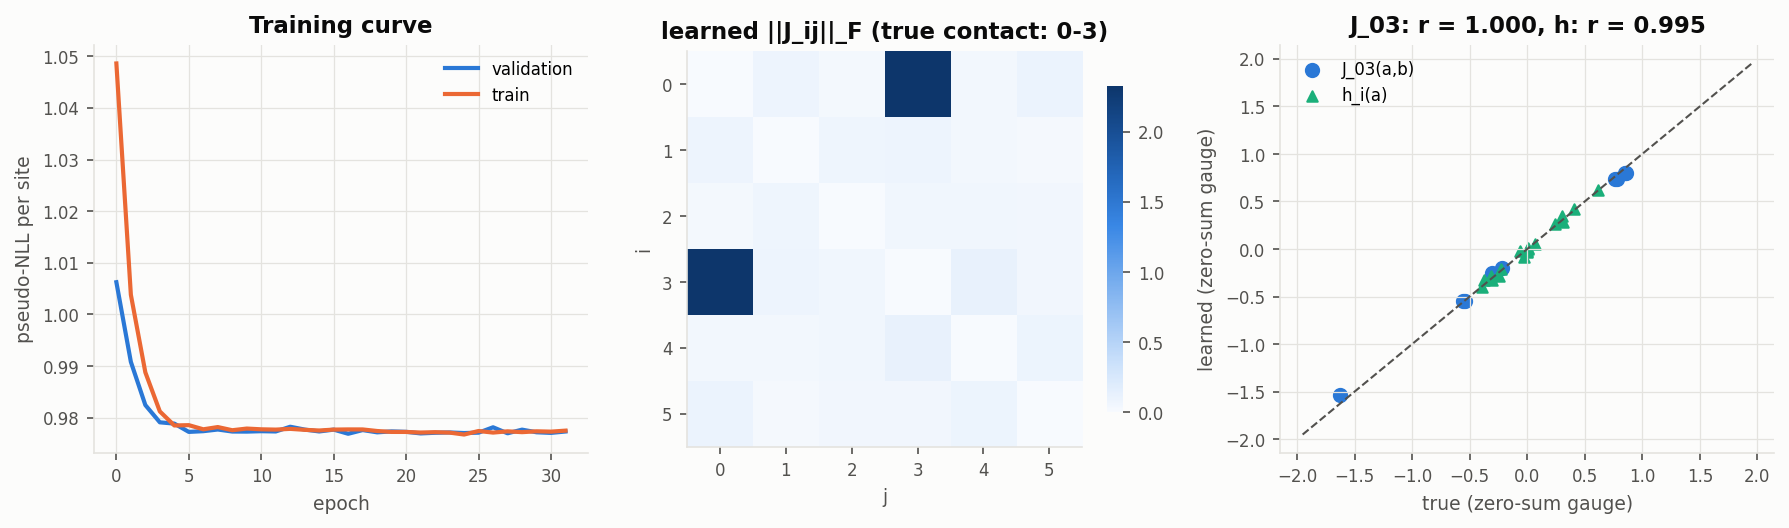
\includegraphics[width=\linewidth]{tests/test_08_factored_attention/test_learns_single_contact/toy_single_contact.png}
\caption{\texttt{test\_08}: toy model with $L=6$, $q=3$ and a single strong coupling between sites 0 and 3,
10{,}000 samples, $H=4$ heads. Left: training curve. Middle: the learned $\|J_{ij}\|$ is concentrated on
the true pair. Right: learned vs true $J_{03}(a,b)$ and $h_i(a)$ (zero-sum gauge), $r=1.000$ and $0.995$.}
\end{figure}

\begin{figure}[H]
\centering
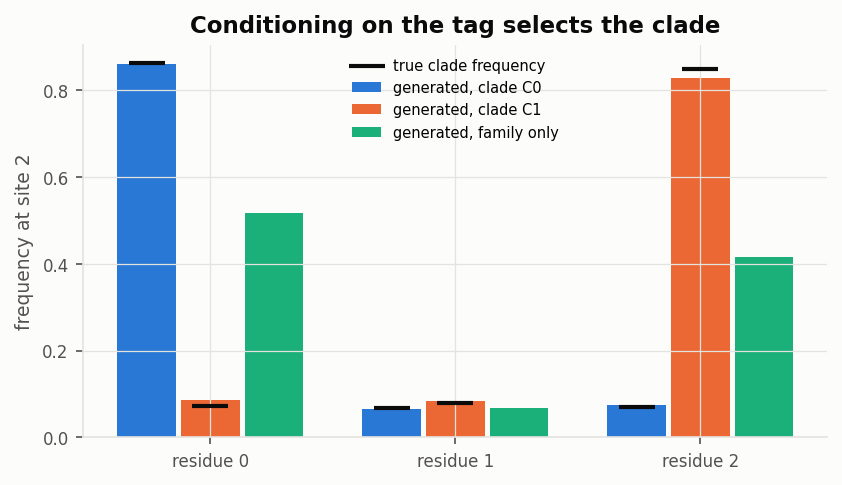
\includegraphics[width=0.62\linewidth]{tests/test_09_conditional/test_learns_clade_specific_fields/site2_by_tag.png}
\caption{\texttt{test\_09}: two clades that prefer residue 0 vs residue 2 at site 2. Sequences generated
with each clade tag reproduce that clade's frequencies (black ticks). With the clade tag dropped (family
only) the model generates the mixture.}
\end{figure}

\begin{figure}[H]
\centering
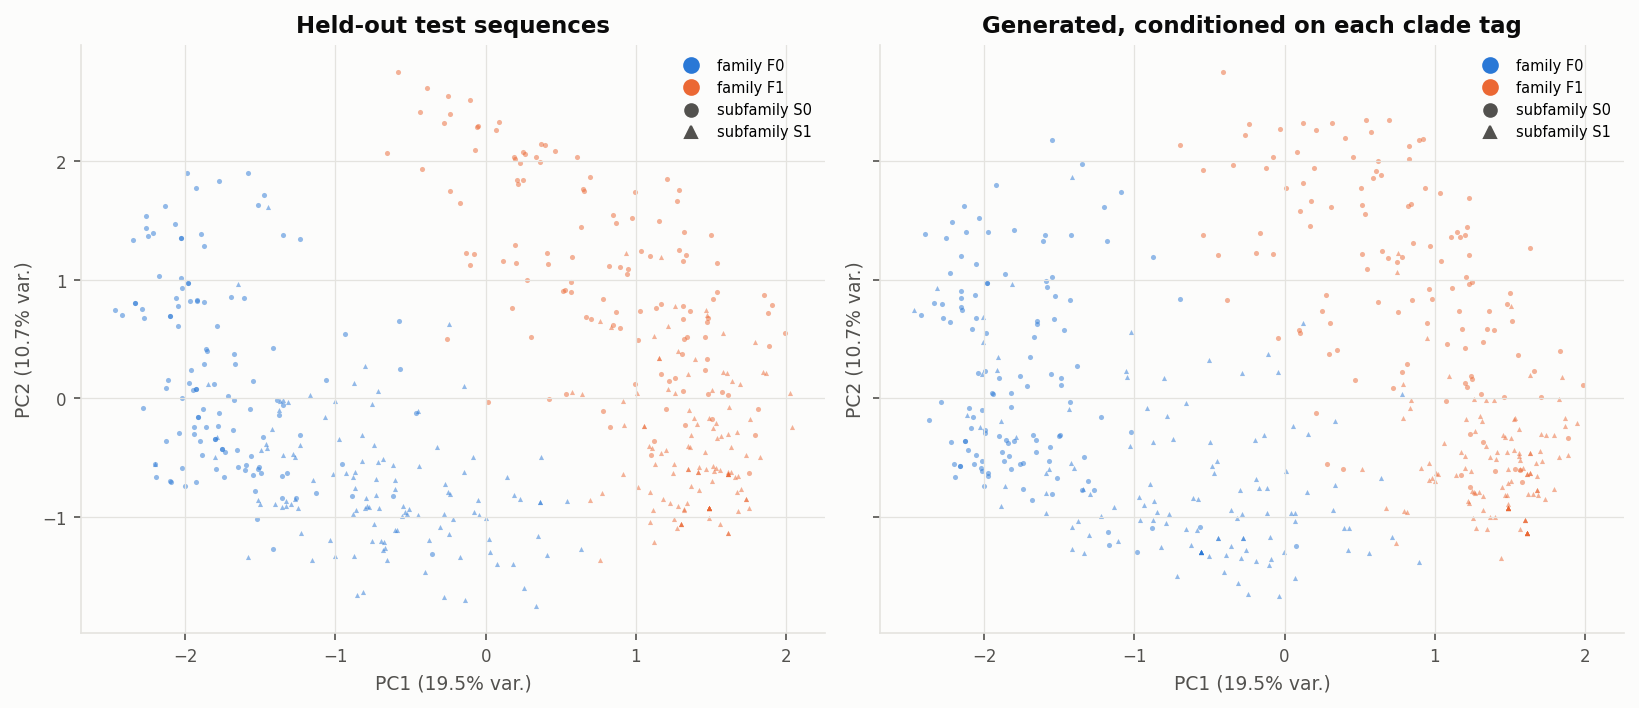
\includegraphics[width=0.9\linewidth]{tests/test_11_model_pipeline/test_model_pipeline_tiny/figures/models/tiny_conditional/pca_generated_vs_test.png}
\caption{\texttt{test\_11}: the full pipeline on a tiny tree ($L=15$, $q=5$, 8 clades) after only 4
epochs. Sequences generated with each clade tag already sit on the test sequences of their family and
subfamily on the reference PCA.}
\end{figure}

%------------------------------------------------------------------------------------------
% Results of the first trained model: unconditioned factored attention, H = 128.
% Numbers from evaluations/fa_unconditional_H128/{metrics,tree_comparison,mode_mixing}.json

\section{Results: the unconditioned model with $H=128$}\label{sec:res_uncond}

\subsection{What was trained}
The unconditioned model of \S\ref{sec:fa} was trained on all 144{,}000 training sequences (18 clades, no tags).
At your request it used $\bm{H=128}$ heads instead of the 256 of the plan, i.e.\ 543{,}920 parameters
(run \texttt{fa\_unconditional\_H128}). Note that 128 is below the $\approx179$ heads that the rank argument
of \S\ref{sec:rank} requires for an exact representation of our couplings. Everything else is as in
\S\ref{sec:plan}: pseudo-likelihood with $\lambda_h=\lambda_J=10^{-5}$, Adam ($5\times10^{-3}$), batch 512,
60 epochs. Training took 98\,s on the RTX~2060.

\begin{figure}[H]
\centering
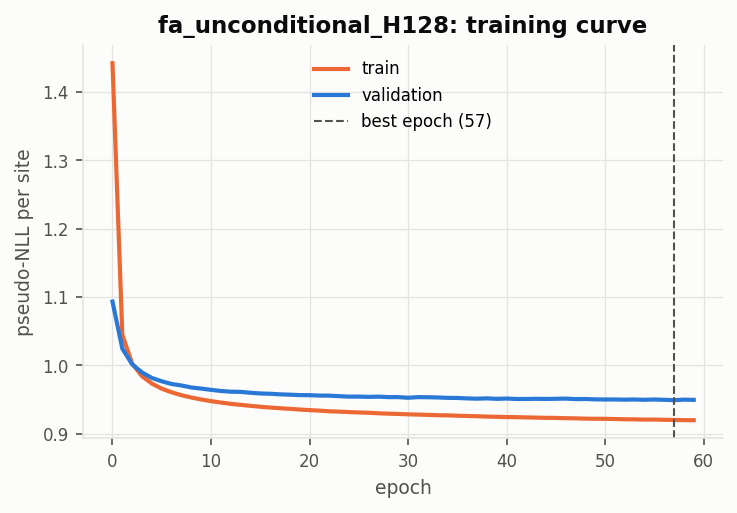
\includegraphics[width=0.55\linewidth]{models/fa_unconditional_H128/training_curve.png}
\caption{Training curve. Best validation pseudo-NLL per site: $0.949$ (epoch 57 of 60). It was still
decreasing slowly at the 60-epoch cap. The train/validation gap is small ($0.920$ vs $0.949$), so there is
little over-fitting.}
\end{figure}

For comparison (\S\ref{sec:plan}): an independent-site model scores 2.11, and the true clade models 0.80.
The unconditioned model reaches $0.95$. That is far better than independent sites, and it cannot reach
0.80, because a single Potts model cannot represent the mixture of 18 clade models.

Evaluation protocol (\S\ref{sec:evalprotocol}): 18{,}000 sequences Gibbs-sampled from the learned $(h,J)$
(200 sweeps, one sequence per chain), compared with the 18{,}000 held-out test sequences. The
\emph{oracle} is 18{,}000 fresh samples of the true clade models (1000 per clade), the best achievable score.

\subsection{Site frequencies and correlations}
\begin{center}\small
\begin{tabular}{lccccc}
\toprule
compared with the test set & $r_f$ & $r_C$ & slope $C$ & identity gen--gen & copies\\
\midrule
oracle (fresh true samples) & 1.000 & 0.994 & 0.99 & 0.197 & 0\%\\
\textbf{generated} & \textbf{0.940} & \textbf{0.895} & \textbf{0.70} & \textbf{0.260} & 0\%\\
generated, rebalanced to equal family shares$^\ast$ & 0.992 & 0.949 & 0.79 & 0.209 & 0\%\\
\bottomrule
\end{tabular}\\[2pt]
{\footnotesize $^\ast$ 2101 generated sequences from each family (see \S\ref{sec:res_props}); identity of the test set itself: 0.198.}
\end{center}

\begin{figure}[H]
\centering
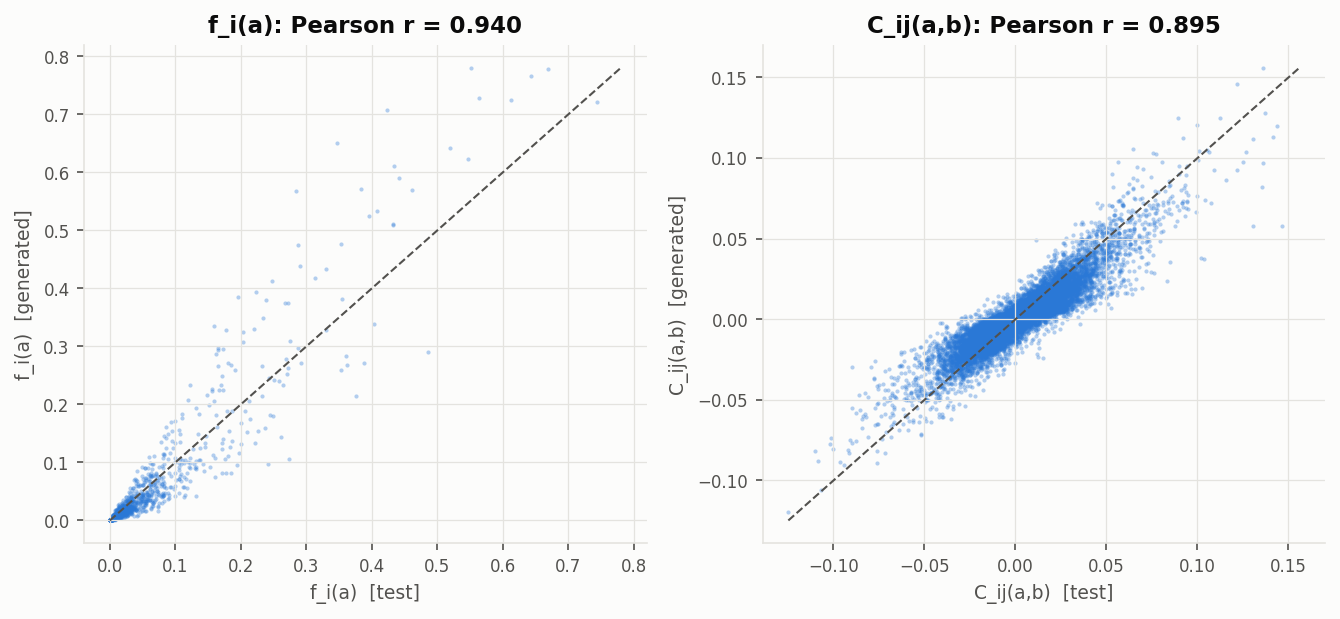
\includegraphics[width=0.49\linewidth]{models/fa_unconditional_H128/freq_corr_generated_vs_test.png}\hfill
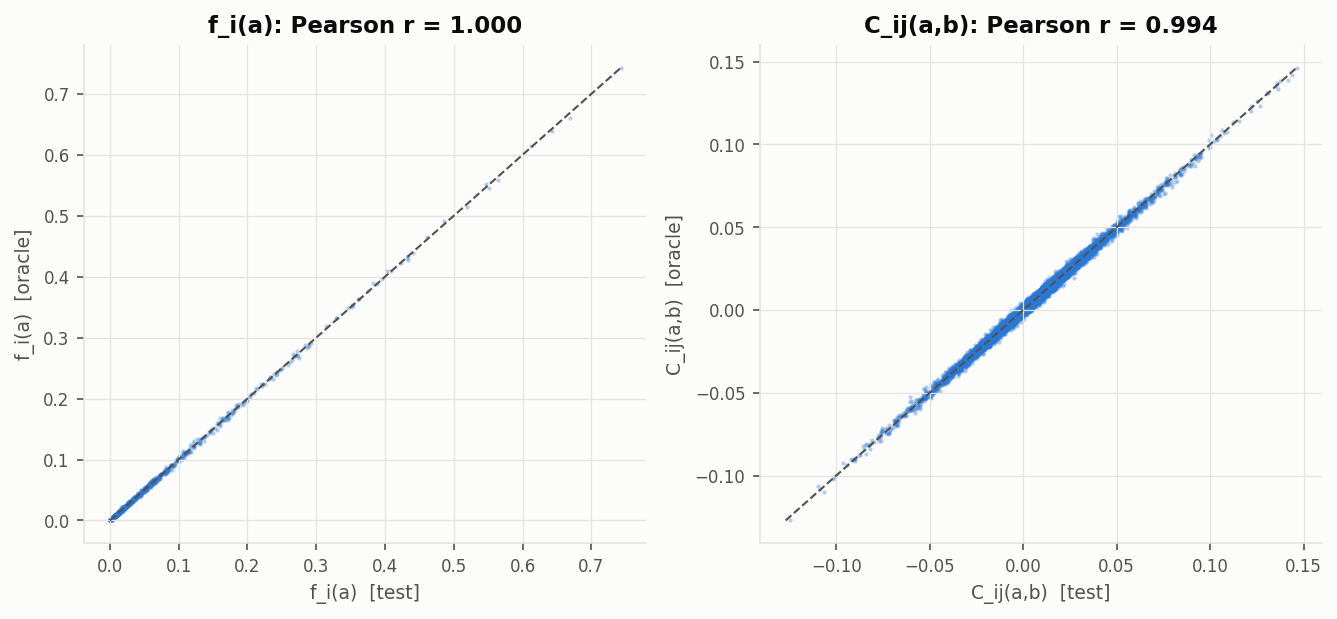
\includegraphics[width=0.49\linewidth]{models/fa_unconditional_H128/freq_corr_oracle_vs_test.png}
\caption{Site frequencies $f_i(a)$ and connected correlations $C_{ij}(a,b)$ of the generated sequences
(left pair) and of the oracle (right pair) against the test sequences. Points on the dashed line are
reproduced exactly.}
\end{figure}

\begin{figure}[H]
\centering
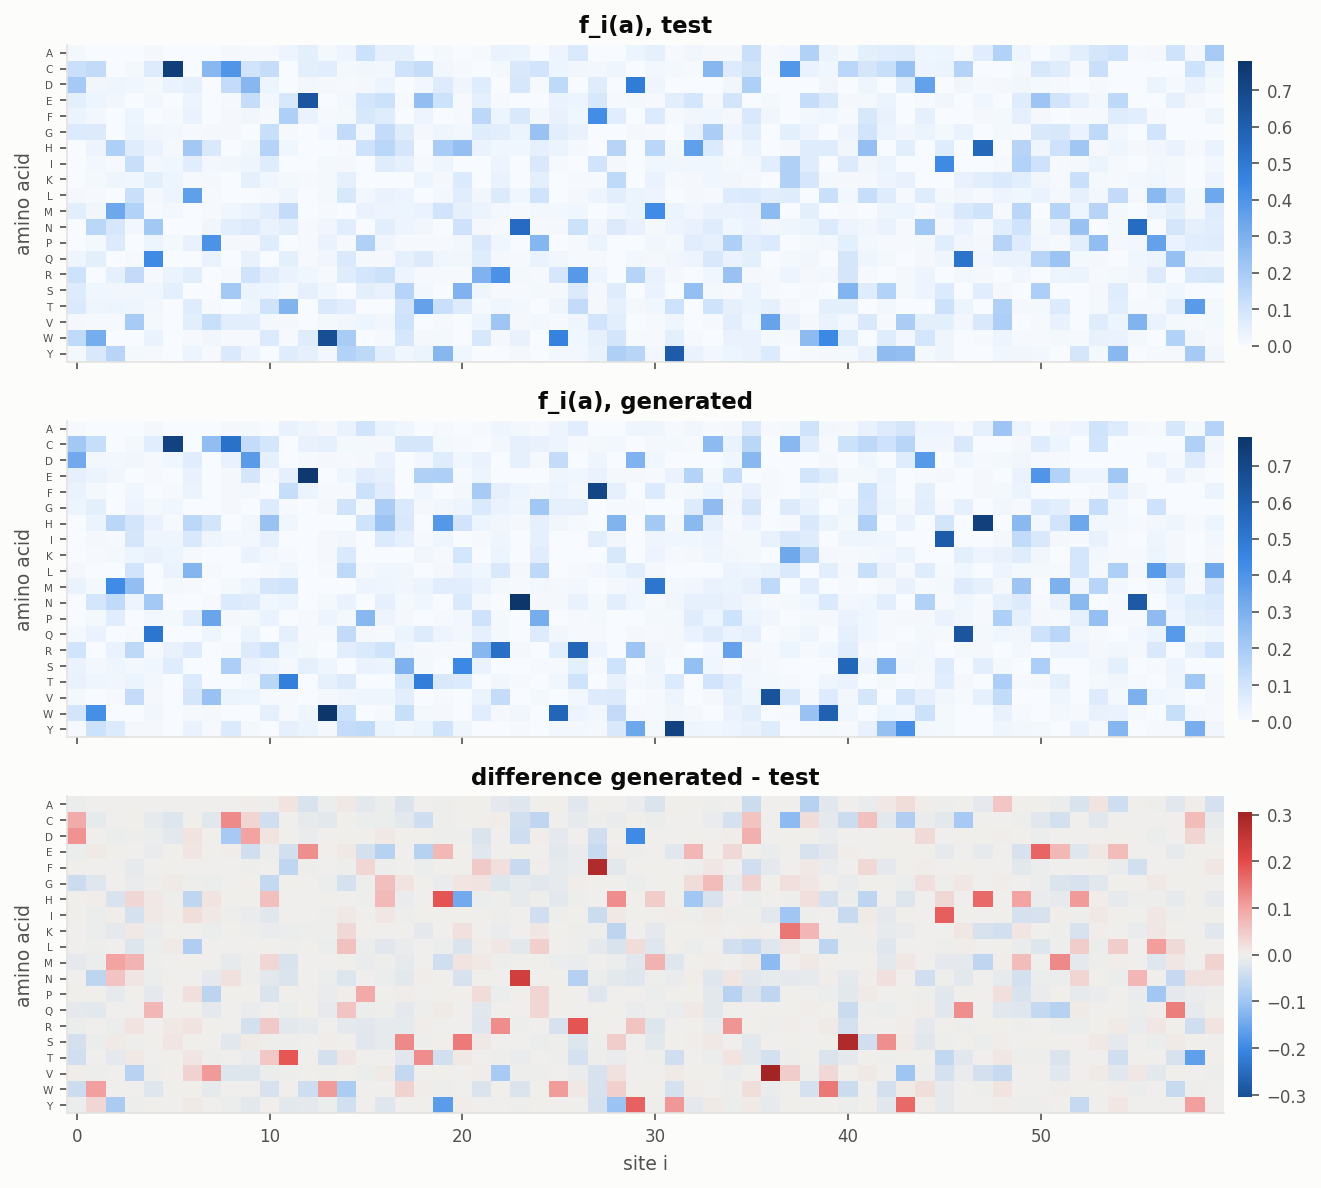
\includegraphics[width=0.78\linewidth]{models/fa_unconditional_H128/site_frequencies_test_vs_generated.png}
\caption{Site frequencies of the test set, of the generated set, and their difference (red: too frequent
in the generated sequences, blue: too rare). The errors are concentrated on a few residues at a few sites.
These are the residues that distinguish the families (next subsection).}
\end{figure}

\begin{figure}[H]
\centering
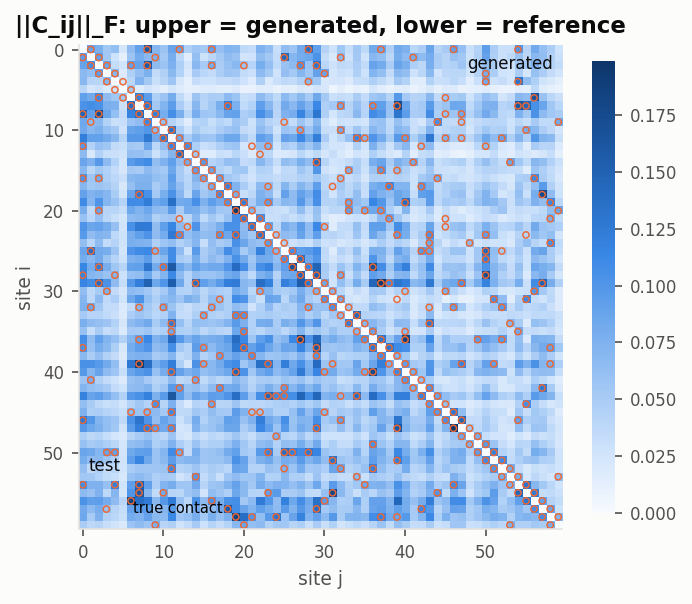
\includegraphics[width=0.5\linewidth]{models/fa_unconditional_H128/correlation_strength_test_vs_generated.png}
\caption{Strength of the correlation between every pair of sites, $\|C_{ij}\|_F$. Lower triangle: test set;
upper triangle: generated; circles: true contacts. In the \emph{pooled} data almost all pairs are correlated,
not only contacts: sites whose preferred residue differs between families become correlated through the
family identity (the mixture effect of \S\ref{sec:cond}). The generated set reproduces this background and the
strongest contact correlations.}
\end{figure}

\subsection{Family proportions: the main failure}\label{sec:res_props}
Each generated sequence is assigned to the family whose test centroid is nearest on the reference PCA (all 10
components). Sequences farther from every centroid than 99\% of the test sequences are from their own
centroid count as ``between families'' (\texttt{family\_assignment}).
\begin{center}\small
\begin{tabular}{lcccc}
\toprule
 & F0 & F1 & F2 & between\\
\midrule
test & 33.0\% & 32.7\% & 33.3\% & 1.0\%\\
oracle & 33.1\% & 32.7\% & 33.3\% & 0.9\%\\
\textbf{generated} & \textbf{21.7\%} & \textbf{11.6\%} & \textbf{66.4\%} & 0.3\%\\
\bottomrule
\end{tabular}
\end{center}

\begin{figure}[H]
\centering
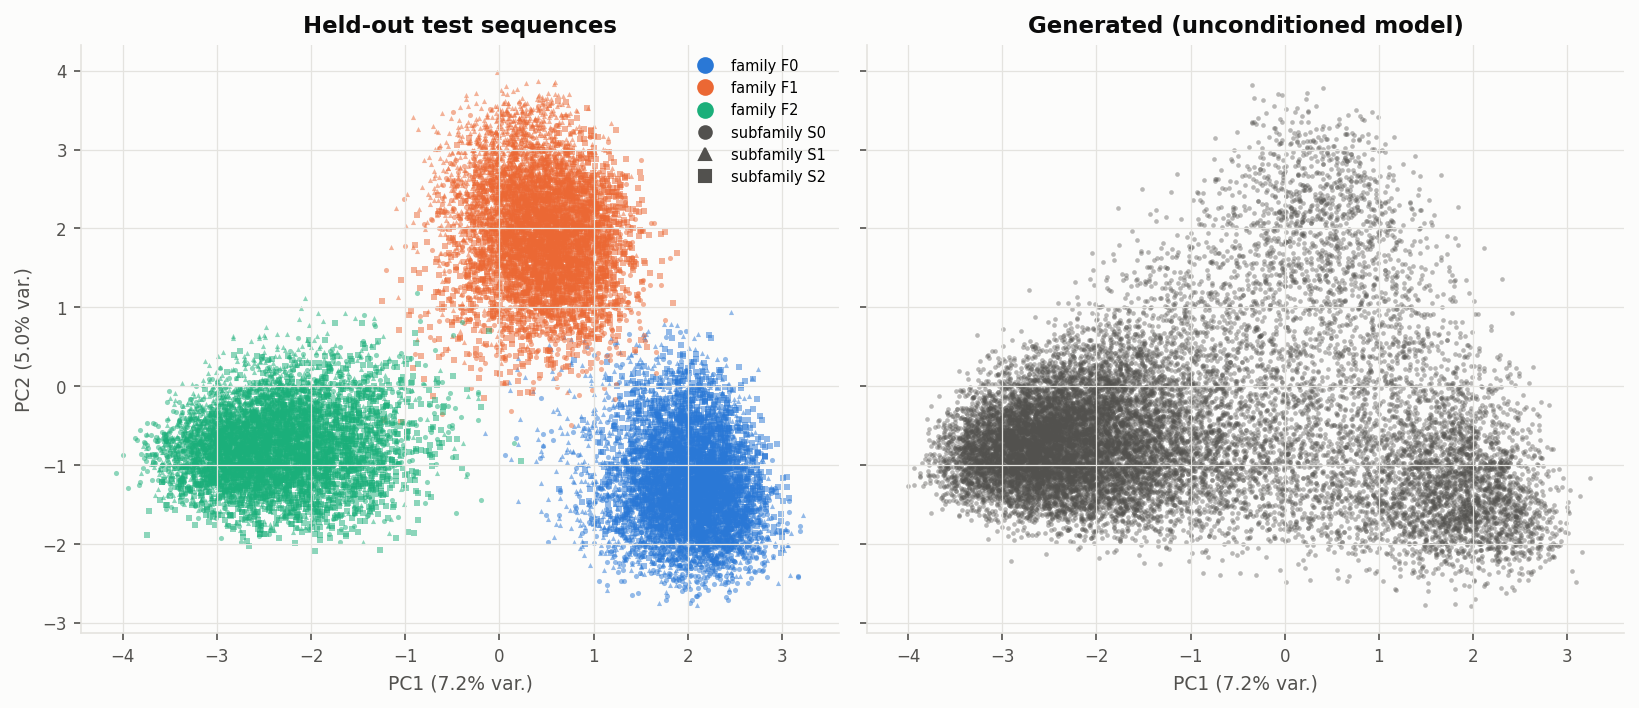
\includegraphics[width=0.85\linewidth]{models/fa_unconditional_H128/pca_generated_vs_test.png}
\caption{Test sequences (left, coloured by family) and generated sequences (right) on the reference PCA
axes of Part~I. The generated sequences occupy all three family regions, with the wrong weights: F2
(bottom left) is over-populated and F1 (top) under-populated.}
\end{figure}

\paragraph{Is it the model or the sampler?} With three well-separated families, a Gibbs chain could get
trapped in whichever family it falls into first. The proportions would then reflect the starting
points, not the learned distribution. We tested this (\texttt{s08\_mode\_mixing.py}): 600 chains were
started from random sequences, and 600 from the test sequences of each family. We then tracked where the
chains are after 100--500 sweeps.
\begin{figure}[H]
\centering
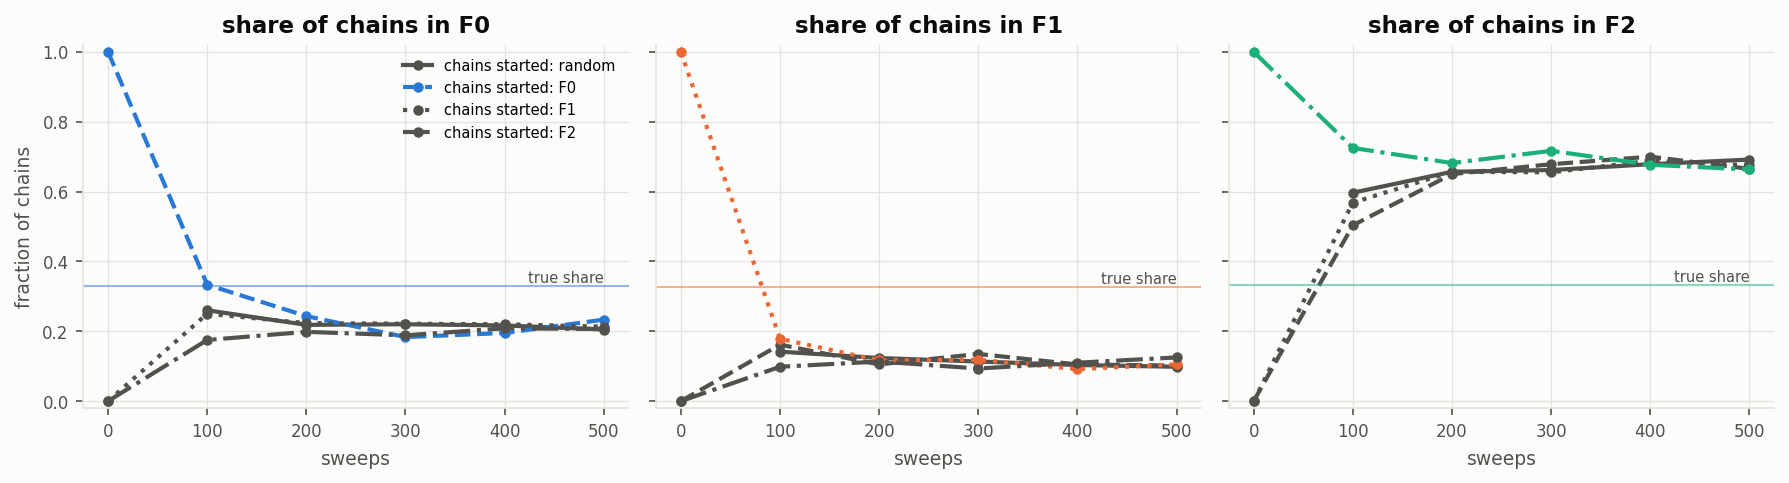
\includegraphics[width=\linewidth]{models/fa_unconditional_H128/mode_mixing.png}
\caption{Share of chains in each family vs sweeps, for chains started at random or inside F0, F1 or F2.
Chains started inside F0 or F1 leave it within 100--200 sweeps. All four starts converge to the same
$\approx20/11/68\%$ split. Horizontal lines: the true share $1/3$.}
\end{figure}
All starts converge to the same proportions, so \textbf{the sampler mixes between families and the
$20/11/68$ split is a property of the learned distribution itself.} Why would pseudo-likelihood learn wrong
family weights? The PL \eqref{eq:pl} only involves the conditionals $P(s_i\mid\s_{-i})$, which never compare
two \emph{different} regions of sequence space. The relative weight of two families is the ratio of the
total Boltzmann weight in each region, a global quantity set by $Z$, which PL never sees. As long as each
family's sequences are predicted well site by site, PL is nearly blind to how much weight each family
receives. This is a known weakness of PLM on multimodal data. The conditioned model avoids it by
construction, since the tag chooses the family.

\paragraph{Is it an energy effect? (``the sampler minimises the energy'')} Figure~\ref{fig:energytraces} shows that the clades of
F2 have the lowest mean energy, and F2 is the over-generated family, so it is natural to suspect that
sampling favours low energy. The link is real, but the mechanism is different. Two facts first:
\begin{itemize}[nosep]
\item Gibbs sampling does \emph{not} minimise the energy. It draws $\s$ with probability $e^{-E(\s)}/Z$
(validated against exact enumeration, \S\ref{sec:gibbstests}). High-energy sequences are rarer, not
excluded.
\item Figure~\ref{fig:energytraces} compares each clade under \emph{its own} model, and the clades were sampled
\emph{separately}. There the families never compete, which is why the oracle has exactly 1/3 in each.
\end{itemize}
In the learned (single) model, however, the three families do compete. The weight of family $F$ is the sum of
the Boltzmann weights of all sequences in its region:
\begin{equation}\label{eq:freeenergy}
P(F)=\frac1Z\sum_{\s\in F}e^{-E(\s)}=\frac1Z\,e^{-(\langle E\rangle_F-S_F)}
\quad\Longrightarrow\quad
\ln\frac{P(F)}{P(F')}=\underbrace{-\big(\langle E\rangle_F-\langle E\rangle_{F'}\big)}_{\text{energy term}}
+\underbrace{\big(S_F-S_{F'}\big)}_{\text{entropy term}}
\end{equation}
where $\langle E\rangle_F$ is the mean energy of the model restricted to region $F$ and $S_F$ its entropy,
i.e.\ the logarithm of the effective number of sequences in $F$. (The second equality defines $S_F$: write
$\sum_{\s\in F}e^{-E}=e^{-\langle E\rangle_F}\sum_{\s\in F}e^{-(E-\langle E\rangle_F)}$ and call the log of the
last sum $S_F$. It is exactly the Gibbs entropy of the restricted distribution.) A family can therefore win
either by having low energies or by having many sequences. We measured the energy term with 2400 samples of the
learned model and obtained the entropy term as the remainder (\texttt{s08\_mode\_mixing.py}):
\begin{center}\small
\begin{tabular}{lccccc}
\toprule
family & $\langle E\rangle_F$ & energy term & entropy term & $\ln\frac{P(F)}{P(\text{F2})}$ & site entropy\\
 & (learned model) & vs F2 & vs F2 & & (test seqs)\\
\midrule
F0 & $-176.1$ & $-10.7$ & $+9.6$ & $-1.12$ & 1.87\\
F1 & $-173.1$ & $-13.7$ & $+12.1$ & $-1.60$ & 1.94\\
F2 & $-186.8$ & 0 & 0 & 0 & 1.57\\
\bottomrule
\end{tabular}
\end{center}
F2 is the most conserved family: lowest site entropy, highest identity (0.36). Hence, in the learned model,
its sequences have $\approx11$--14 units lower energy, but its region also holds far fewer sequences. The two
effects almost cancel: an energy advantage worth a factor $e^{11}\approx60{,}000$ is reduced to a factor
$\approx3$--5 by the entropy. So \textbf{your intuition is right that the low energy of F2 is what favours it},
and it has the same origin as its low energy in Figure~\ref{fig:energytraces} (strong conservation). But the imbalance is the
small \emph{residual} of a near-cancellation between energy and entropy, not an energy minimisation. Equal
weights would need the two terms to cancel to within $\approx0.1$ nat. Pseudo-likelihood has no term that
enforces this, because the balance is a property of $Z$. That is the precise sense of the ``PL does not see
$Z$'' statement above.

\paragraph{Inside each family the sequences are good.} Taking the generated sequences assigned to each
family and comparing them with that family's test sequences:
\begin{center}\small
\begin{tabular}{lccccc}
\toprule
family & $n$ generated & $r_f$ & $r_C$ & slope $C$ & identity gen / test\\
\midrule
F0 & 3938 & 0.977 & 0.819 & 0.63 & 0.247 / 0.261\\
F1 & 2101 & 0.968 & 0.784 & 0.63 & 0.217 / 0.236\\
F2 & 11961 & 0.993 & 0.896 & 0.73 & 0.350 / 0.363\\
\bottomrule
\end{tabular}
\end{center}
The frequencies inside each family are right ($r_f\ge0.97$), and rebalancing the generated set to equal
family shares brings the pooled $r_f$ from 0.94 to 0.99 and the identity from 0.260 to 0.209 (table
above). So \textbf{most of the frequency error and most of the excess identity come from the wrong family
weights}; the remaining excess, 0.209 vs 0.198, is small. (The pooled identity was too high because F2, the most over-represented family, is also the
most internally similar one: 0.36.) What remains is that \textbf{correlations are too weak}: the slope of
generated vs test $C$ is 0.63--0.73 inside families, and 0.79 after rebalancing. This matches the shrunken
couplings found below.

\subsection{The learned $J$ compared with every $J$ of the tree}
We compare the learned couplings, in the zero-sum gauge, with each of the 31 ground-truth models. These are
the \textbf{root}, the ancestor from which all others were generated, then the 3 families, the 9 subfamilies
and the 18 clades, plus the average of the 18 clade models (\texttt{s07\_compare\_to\_tree.py}).

\begin{figure}[H]
\centering
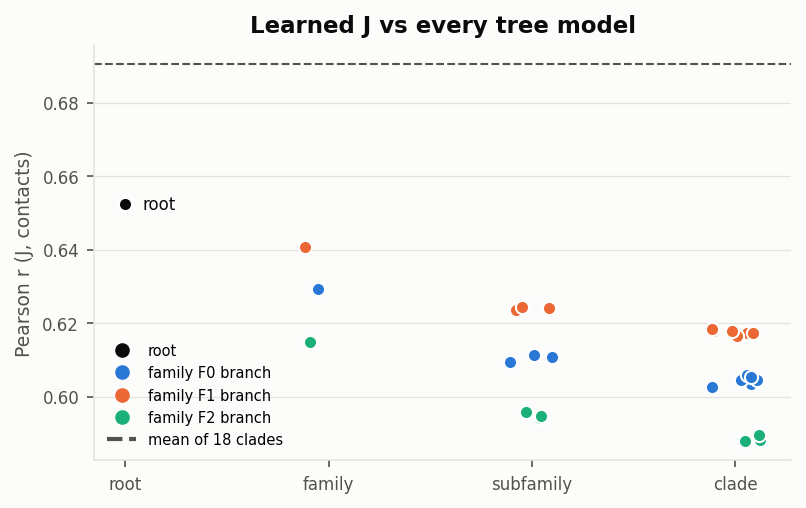
\includegraphics[width=0.49\linewidth]{models/fa_unconditional_H128/tree_rJ.png}\hfill
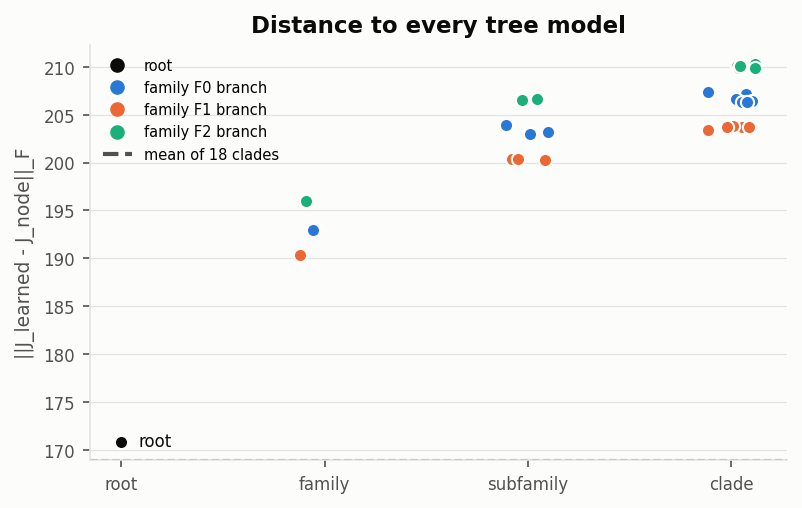
\includegraphics[width=0.49\linewidth]{models/fa_unconditional_H128/tree_dJ.png}
\caption{Learned $J$ vs every model of the tree, grouped by level, coloured by family branch. Left: Pearson
correlation on the contact entries. Right: distance $\|J^0_{\text{learned}}-J^0_{\text{node}}\|_F$. Dashed:
the average of the 18 clade models.}
\label{fig:treeJ}
\end{figure}

\begin{center}\small
\begin{tabular}{lccccc}
\toprule
compared with & $r_J$ (contacts) & slope & $d_J$ & $r_h$ & $d_h$\\
\midrule
average of the 18 clades & \textbf{0.691} & 0.57 & \textbf{168.9} & \textbf{0.922} & \textbf{26.3}\\
root (ancestor) & 0.652 & 0.57 & 170.9 & 0.865 & 27.5\\
family F0 & 0.629 & 0.48 & 192.9 & 0.836 & 36.2\\
family F1 & 0.641 & 0.49 & 190.3 & 0.857 & 35.3\\
family F2 & 0.615 & 0.47 & 196.0 & 0.802 & 39.3\\
subfamilies (range) & 0.594--0.624 & 0.43--0.46 & 200--207 & 0.78--0.84 & 38--42\\
clades (range) & 0.588--0.618 & 0.42--0.45 & 203--210 & 0.77--0.83 & 39--44\\
\bottomrule
\end{tabular}
\end{center}

\begin{figure}[H]
\centering
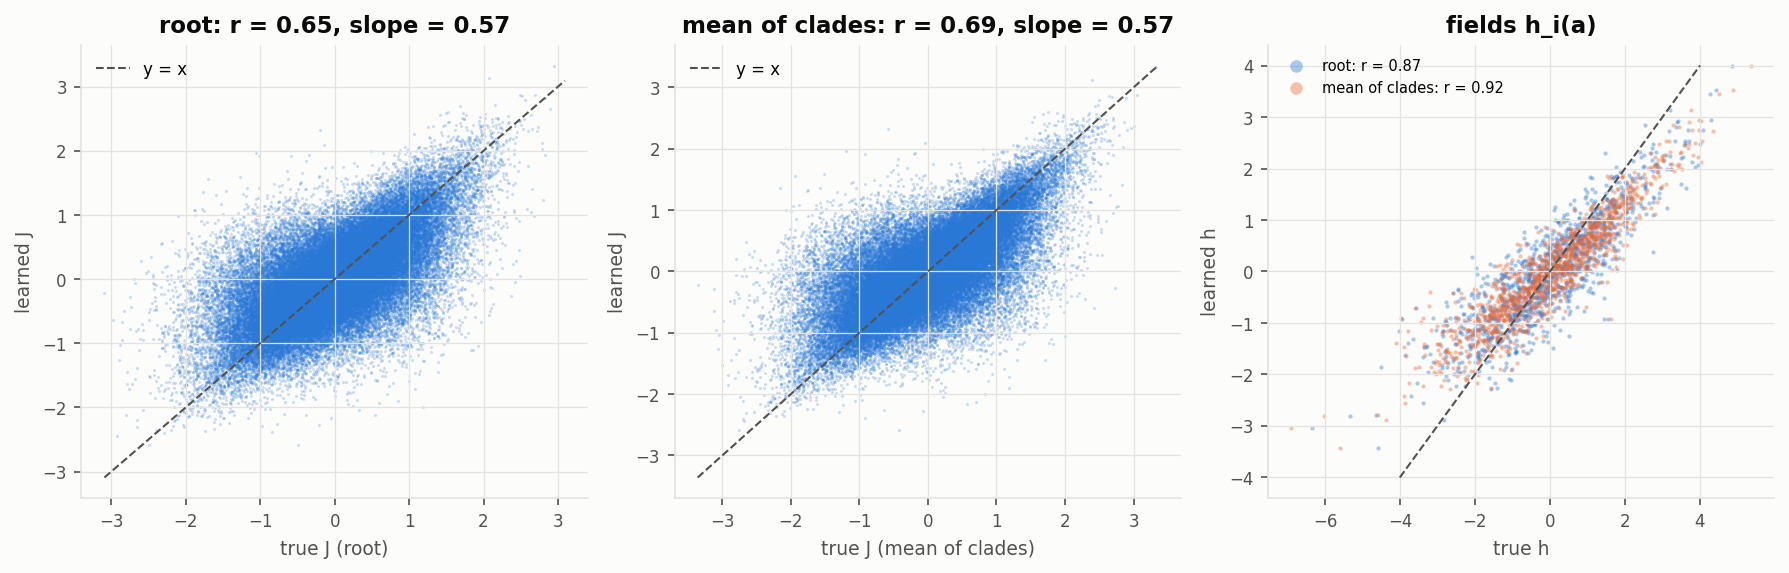
\includegraphics[width=\linewidth]{models/fa_unconditional_H128/tree_scatter_J.png}
\caption{Learned vs true couplings on the contact entries, for the root and for the average of the clades,
and learned vs true fields. The cloud is centred on a line of slope $\approx0.57$, below the diagonal.}
\end{figure}

\paragraph{Reading.}
\begin{enumerate}
\item \textbf{The model learned the common ancestor, not any family.} The similarity decreases
monotonically down the tree: root/average of clades $>$ families $>$ subfamilies $>$ clades
(Figure~\ref{fig:treeJ}). This is what one expects from fitting one Potts model to all 18 clades: the part of
$J$ shared by everyone is the ancestral part, and the family- and clade-specific perturbations average out.
The best match is the average of the clades ($r_J=0.69$), which is itself close to the root (distance 71,
against $\|J_{\text{root}}\|=202$).
\item \textbf{F2 is the \emph{least} similar family}, although it is the most over-generated. The wrong
family weights are therefore not caused by $J$ resembling F2. They sit in the global balance of $h$ and
$J$ that PL does not constrain.
\item \textbf{The couplings are too weak and partly misplaced.} The slope is 0.57: along the direction of
the true couplings, the learned ones have about 57\% of the true magnitude. This is the source of the
too-weak correlations. The distance to the root, 171, splits into 160 on the true contacts and 61 on
non-contacts, where the truth is zero but the learned model has spread couplings (mean $|J|=0.06$). The
learned contact couplings have almost the right total size (177 vs 202), but only part of them is aligned
with the true ones. The rest encodes the mixture: extra couplings that tie together the residues typical of
each family. That is exactly how a single Potts model can mimic a mixture.
\item \textbf{The contact map is found perfectly.} All 120 true long-range contacts are the 120 top-ranked
pairs by $\|J_{ij}\|$ with APC (precision $1.00$). This holds even with $H=128<179$ heads. The heads are
enough to locate every contact, though not to reproduce every coupling value.
\item The fields agree well with the average of the clades ($r_h=0.92$): conservation is learned correctly.
\end{enumerate}

\subsection{Summary of the first run}
\begin{keybox}{Unconditioned model with $H=128$}
\begin{itemize}[nosep]
\item[+] Finds all true contacts; site frequencies inside each family are right; no copies of test
      sequences; pooled correlations $r_C=0.90$ (0.95 once family shares are corrected).
\item[--] \textbf{Wrong family weights} (22/12/66\% instead of 33/33/33\%). This is a property of the
      learned distribution, not of the sampler, and is explained by pseudo-likelihood not seeing $Z$.
\item[--] Correlations about 20--35\% too weak (slope 0.63--0.79), because the couplings are shrunk
      (slope 0.57) and partly spent on representing the mixture.
\item[$\to$] Its $J$ is closest to the \emph{ancestral} (root) and \emph{average} models, and gets steadily
      further from the family, subfamily and clade models. It learned what all clades share.
\end{itemize}
Natural next steps: the conditioned model (tags fix the family weights and allow clade-specific $J$);
$H=256$ and/or more epochs to see how much of the shrinkage is capacity vs the mixture.
\end{keybox}


% Results of the conditioned model with hierarchical tags, H = 128.
% Numbers from evaluations/fa_conditional_H128/{metrics,tree_comparison,mode_mixing}.json

\section{Results: the conditioned model with $H=128$}\label{sec:res_cond}

\subsection{What was trained}
The conditioned model of \S\ref{sec:cond} (hierarchical tags, shared attention, label-specific $\Delta h$ and
$\Delta V$, hierarchical tag dropout 0.10/0.10/0.15) was trained on the same 144{,}000 sequences, with
$\bm{H=128}$ heads like the unconditioned run, so that the two differ only by the conditioning
(run \texttt{fa\_conditional\_H128}, 2{,}115{,}920 parameters, of which 1{,}572{,}000 in the label tables).
Regularisation: $\lambda_h=\lambda_J=10^{-5}$, $\lambda_{\text{label}}=10^{-4}$. Training took 23 minutes and
stopped early at epoch 47. The best epoch is 38.

\begin{figure}[H]
\centering
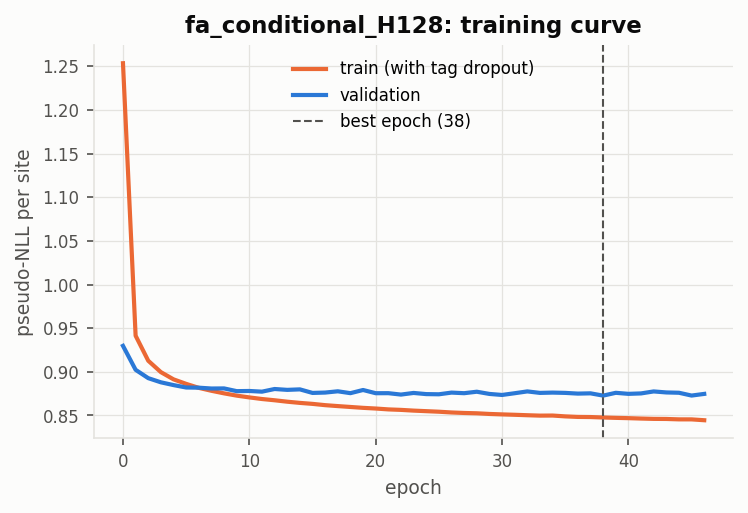
\includegraphics[width=0.55\linewidth]{models/fa_conditional_H128/training_curve.png}
\caption{Training curve. The validation pseudo-NLL (true tags) reaches $0.878$ by epoch 10 and only $0.873$
at the best epoch (38). Meanwhile the training loss keeps decreasing (with tag dropout, so it is not directly
comparable). The label tables start to fit noise beyond epoch $\approx10$.}
\end{figure}

\begin{center}\small
\begin{tabular}{lc}
\toprule
model & validation pseudo-NLL per site\\
\midrule
independent sites, one profile per clade & 1.63\\
unconditioned model ($H=128$) & 0.949\\
\textbf{conditioned model ($H=128$), true tags} & \textbf{0.873}\\
true clade Potts models (floor) & 0.80\\
\bottomrule
\end{tabular}
\end{center}
The tags close about half of the gap between the unconditioned model and the floor.

\subsection{Sequences generated with a clade tag}
For each clade, 1000 sequences were generated with its full tag and compared with that clade's 1000 test
sequences. The oracle is 1000 fresh samples of the true clade model, i.e.\ the noise floor of
\S\ref{sec:refvalues}.
\begin{center}\small
\begin{tabular}{lccccc}
\toprule
mean [min, max] over 18 clades & $r_f$ & $r_C$ & slope $C$ & identity gen / test & copies\\
\midrule
oracle & 0.998 & 0.832 [0.80, 0.88] & 0.84 & 0.337 / 0.337 & 0\%\\
\textbf{generated (clade tag)} & \textbf{0.967} & \textbf{0.758} [0.71, 0.82] & \textbf{0.75} & 0.362 / 0.337 & 0\%\\
\bottomrule
\end{tabular}
\end{center}
On the reference ladder of \S\ref{sec:refvalues} (0.83 same clade, 0.63 sibling clade, 0.35 same family,
0.08 other family), the generated clades score \textbf{0.76}. That is well above the sibling-clade level, so
the generated sequences are closer to their own clade than the true sibling clade is, but still below the
oracle. The generated sequences are slightly too similar to each other (identity 0.36 vs 0.34), and their
correlations are somewhat too weak (slope 0.75 vs 0.84 for the oracle; the oracle slope is below 1 only
because of finite-sample noise).

\begin{figure}[H]
\centering
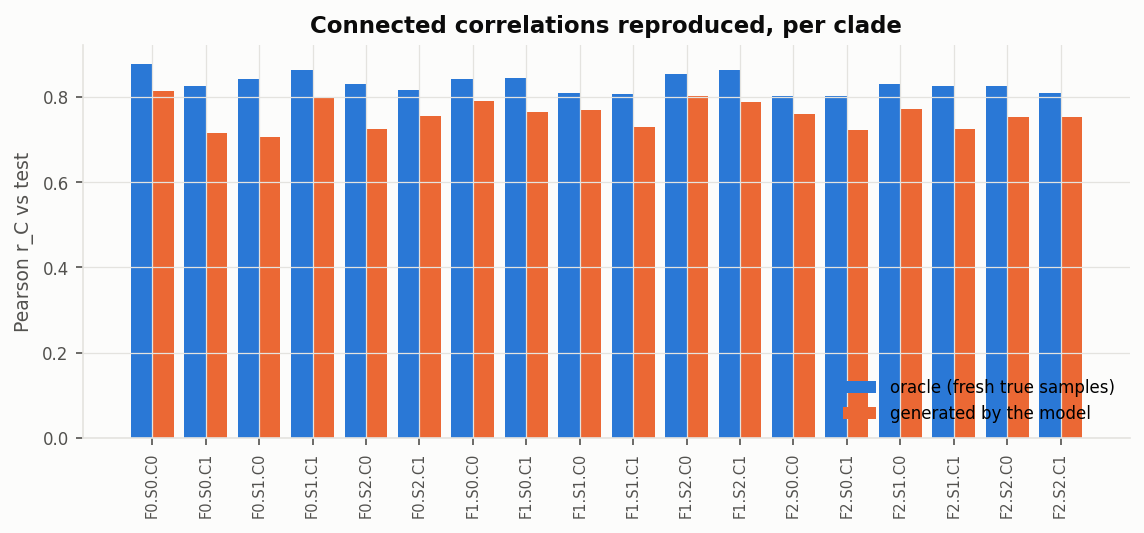
\includegraphics[width=0.8\linewidth]{models/fa_conditional_H128/rC_per_clade.png}
\caption{$r_C$ of each clade's generated sequences vs its test sequences (orange), next to the oracle (blue).
The gap is 0.04--0.14 depending on the clade.}
\end{figure}

\begin{figure}[H]
\centering
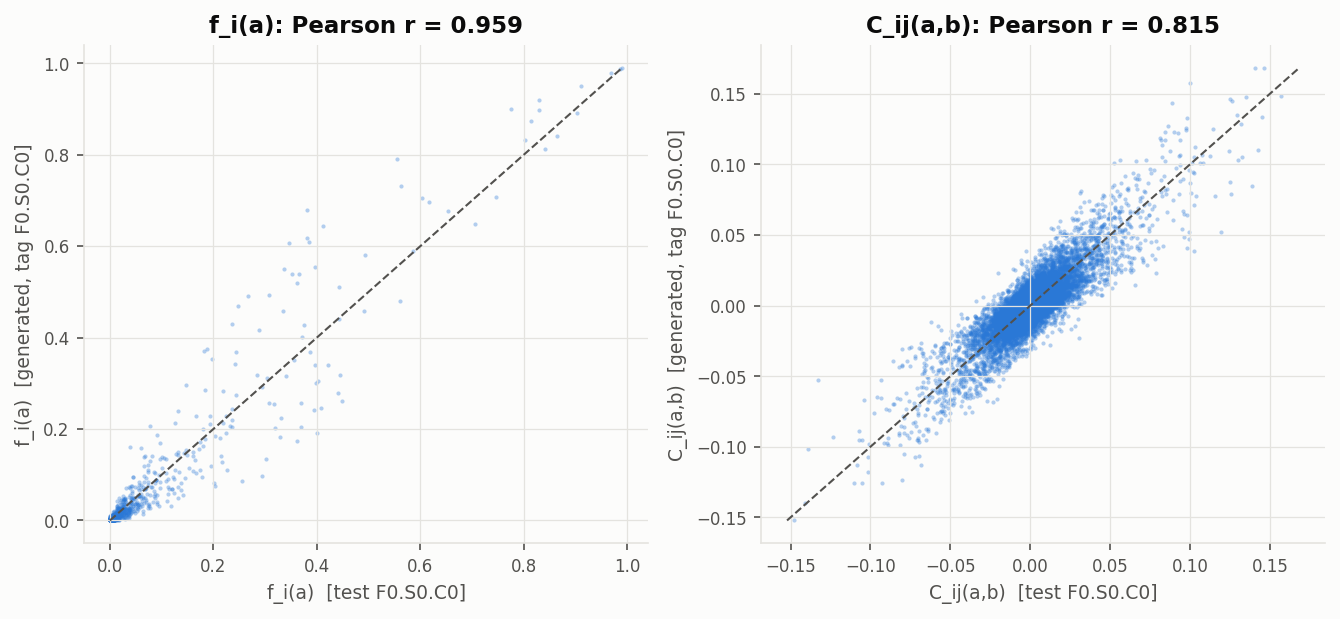
\includegraphics[width=0.49\linewidth]{models/fa_conditional_H128/freq_corr_F0.S0.C0.png}\hfill
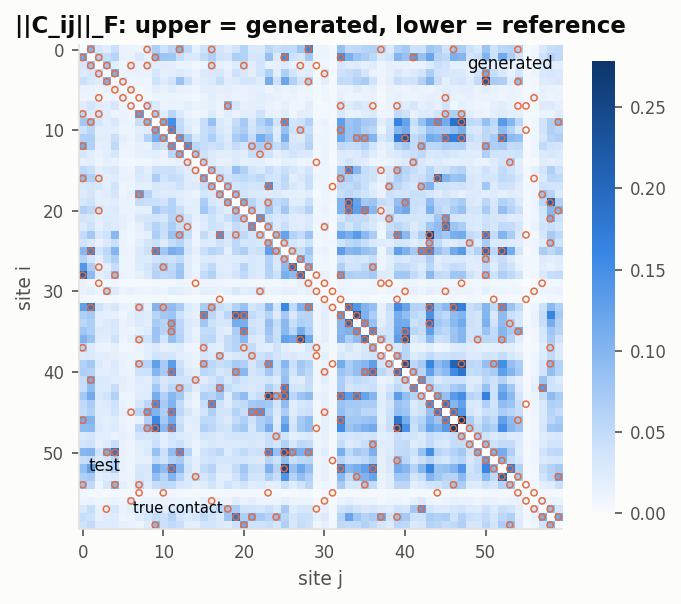
\includegraphics[width=0.4\linewidth]{models/fa_conditional_H128/correlation_strength_F0.S0.C0.png}
\caption{Example clade \texttt{F0.S0.C0}. Left: site frequencies and connected correlations, generated vs
test. Right: correlation strength $\|C_{ij}\|$, test (lower triangle) vs generated (upper), true contacts
circled. Within one clade the strongest correlations sit on true contacts. The weaker background comes from
indirect correlations and finite-sample noise (1000 sequences).}
\end{figure}

\begin{figure}[H]
\centering
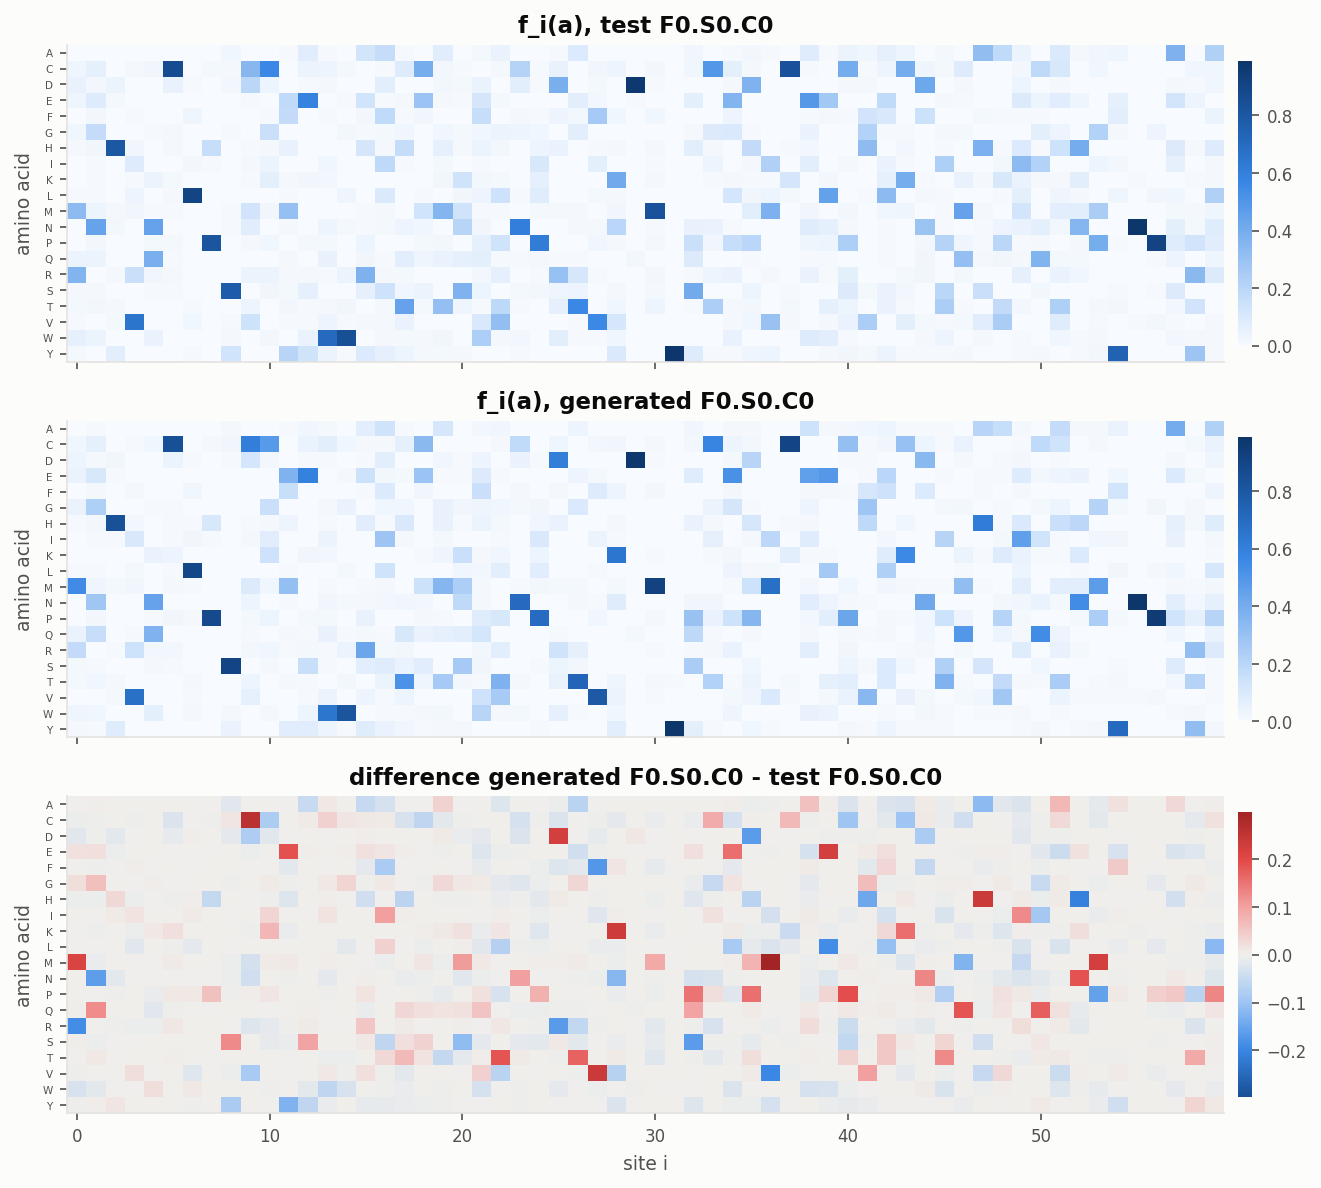
\includegraphics[width=0.78\linewidth]{models/fa_conditional_H128/site_frequencies_F0.S0.C0.png}
\caption{Site frequencies of clade \texttt{F0.S0.C0}: test, generated with its tag, and the difference.}
\end{figure}

\paragraph{Does the tag select the right clade?} For every pair (generated clade $a$, test clade $b$) we
compute $r_C$. \textbf{All 18 generated clades are closest to their own test clade} (assignment accuracy
100\%), and the matrix reproduces the hierarchy of the data: sibling clades next, then the same family.
\begin{figure}[H]
\centering
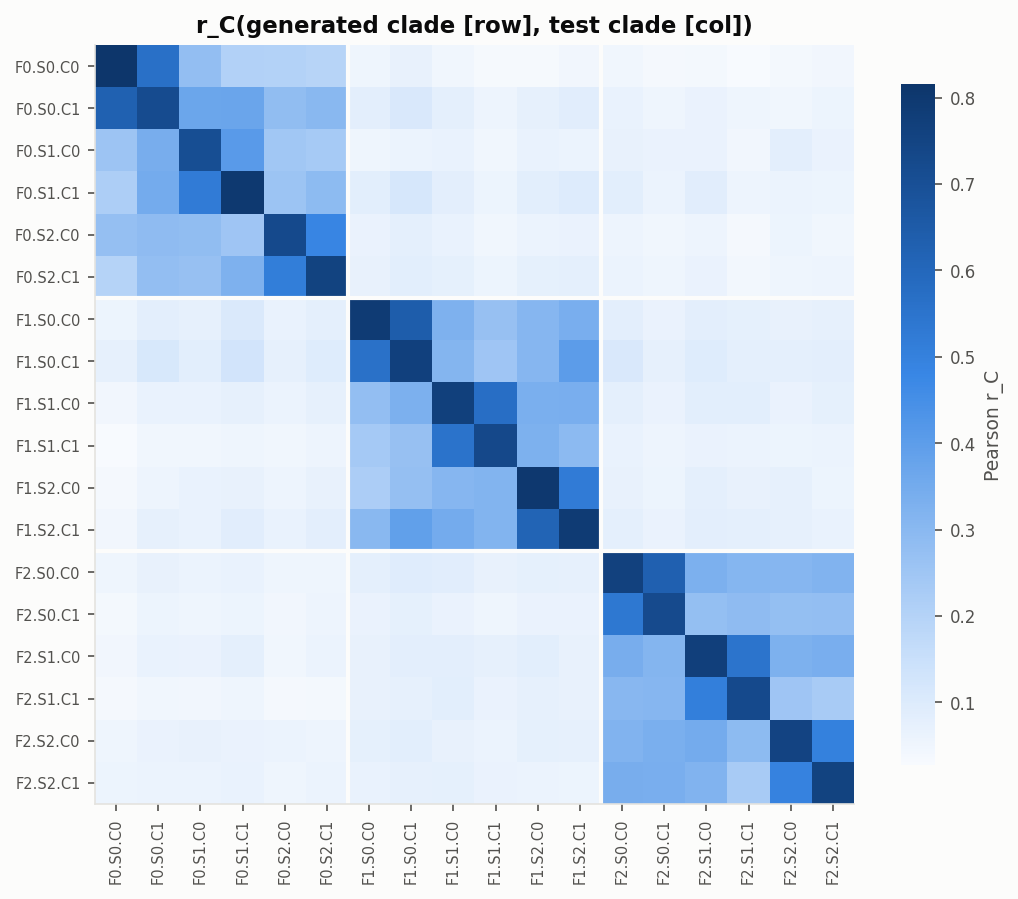
\includegraphics[width=0.62\linewidth]{models/fa_conditional_H128/cross_clade_rC.png}
\caption{$r_C$ between generated clade (row) and test clade (column). The diagonal dominates every row, and
the block structure (pairs of sibling clades, then families) is that of the ground truth.}
\end{figure}

\begin{figure}[H]
\centering
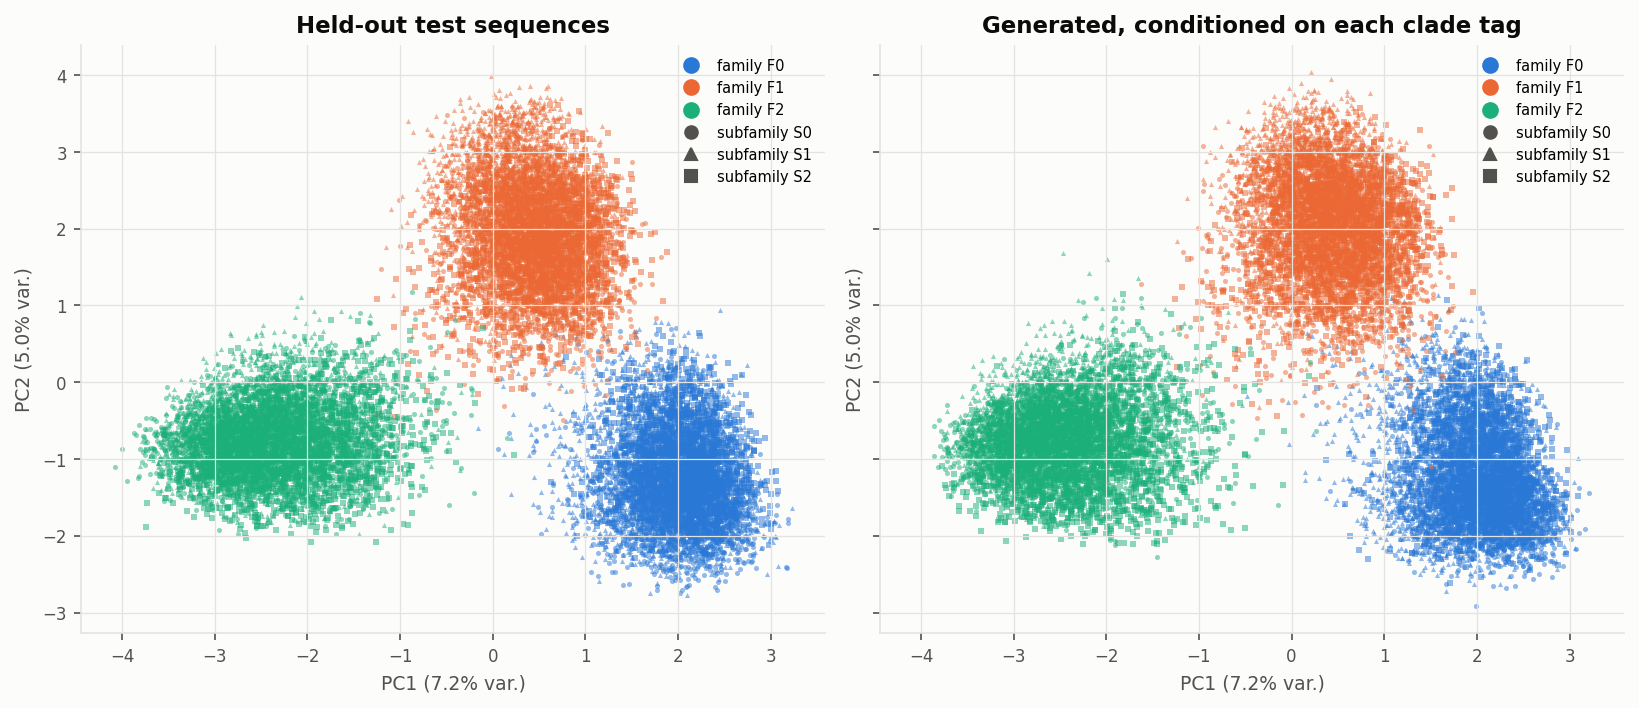
\includegraphics[width=0.85\linewidth]{models/fa_conditional_H128/pca_generated_vs_test.png}
\caption{Test sequences (left) and sequences generated with each of the 18 clade tags (right) on the reference
PCA. Pooled over the 18 tags, the generated set has exactly the right family shares (32.8/32.9/33.3\%) and
$r_f=0.992$, $r_C=0.954$ against the whole test set.}
\end{figure}

\subsection{Sequences generated with a family tag, or with no tag}
\begin{center}\small
\begin{tabular}{lccccc}
\toprule
tag & $r_f$ & $r_C$ & slope $C$ & \multicolumn{2}{c}{family of the generated sequences}\\
\midrule
family F0 only & 0.986 & 0.841 & 0.71 & \multicolumn{2}{c}{99.4\% in F0}\\
family F1 only & 0.984 & 0.856 & 0.73 & \multicolumn{2}{c}{97.8\% in F1}\\
family F2 only & 0.990 & 0.850 & 0.67 & \multicolumn{2}{c}{99.4\% in F2}\\
no tag & 0.980 & 0.872 & 0.52 & \multicolumn{2}{c}{F0/F1/F2 $=$ 33/21/46\%}\\
\bottomrule
\end{tabular}
\end{center}
(Family-tag samples are compared with the whole family's test set, 6000 sequences; no-tag samples with the
whole test set.)
\begin{itemize}
\item \textbf{A family tag generates that family}, 98--99\% of the time, with good statistics. This is
      what the unconditioned model could not do.
\item \textbf{With no tag the family weights are still wrong} (33/21/46\%), although less so than for the
      unconditioned model (22/12/66\%). This is the same pseudo-likelihood blind spot as in
      \S\ref{sec:res_props}. The no-tag mode is fitted to the whole mixture (10\% of training sequences have no
      tag). The energy/entropy breakdown (\texttt{s08}) shows the same near-cancellation as before: relative to F2, F0
      has an energy term $-9.4$ and an entropy term $+9.2$ (net $-0.27$), and F1 has $-14.1$ and $+13.3$ (net
      $-0.77$). With tags, the family weights are \emph{chosen by the user}, so this blind spot no longer matters for
      generation: pooling equal numbers of clade-tag samples gives exactly 1/3 per family (previous figure).
\end{itemize}

\subsection{The learned $J(\text{tag})$ compared with the right tensors}
Each tree node has a tag that should reproduce it: the root $\leftarrow$ no tag; family F$f$ $\leftarrow$
tag $(f,-,-)$; subfamily $\leftarrow$ family $+$ subfamily tag; clade $\leftarrow$ full tag. So we have 31
learned models for 31 true ones. Each learned $J(\text{tag})$ was compared with every true $J$
(\texttt{s07\_compare\_to\_tree.py}); the \emph{matched} comparison is the diagonal.

\begin{figure}[H]
\centering
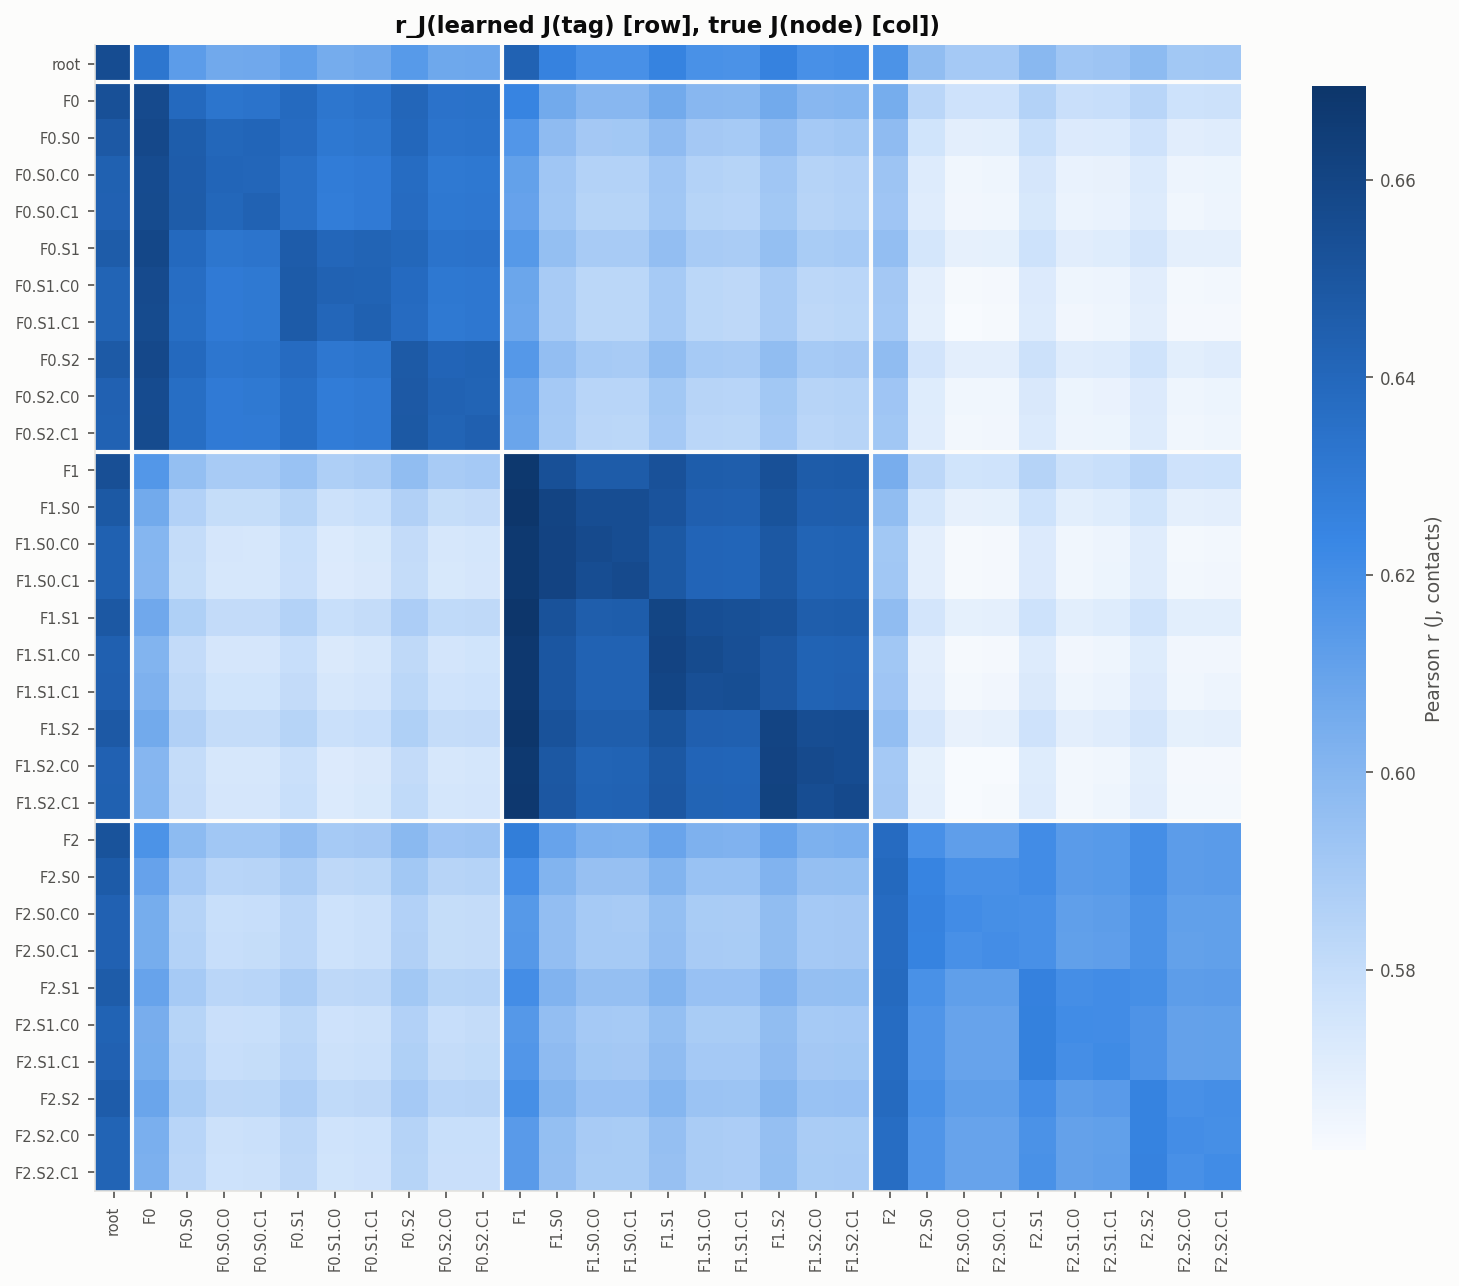
\includegraphics[width=0.8\linewidth]{models/fa_conditional_H128/tree_matrix_rJ.png}
\caption{Pearson $r_J$ (contact entries, zero-sum gauge) between the learned $J$ of each tag (rows) and every
true $J$ (columns). A perfect model would have a dark diagonal. What we see is a clear \emph{family} block
structure: every tag's $J$ resembles its own family (and the root) more than any other family. Within a
family block, however, the rows differ only slightly (a faint subfamily diagonal): the couplings barely
distinguish subfamilies and clades.}
\label{fig:matrixJ}
\end{figure}

\begin{center}\small
\begin{tabular}{lcccccc}
\toprule
level of the tag & $n$ & matched $r_J$ & matched slope & matched $r_h$ & $r(\Delta J)$ & $r(\Delta h)$\\
\midrule
none (root) & 1 & 0.655 & 0.46 & 0.871 & -- & --\\
family & 3 & 0.654 & 0.42 & 0.889 & 0.34 & 0.58\\
subfamily & 9 & 0.644 & 0.41 & 0.882 & 0.21 & 0.50\\
clade & 18 & 0.640 & 0.40 & 0.871 & 0.11 & 0.33\\
\bottomrule
\end{tabular}
\end{center}
Here $r(\Delta J)$ is the correlation between the learned change of couplings from the parent tag to the child
tag, $J(\text{child tag})-J(\text{parent tag})$, and the \emph{true} change $J_{\text{child}}-J_{\text{parent}}$
(contact entries, zero-sum gauge); $r(\Delta h)$ is the same for the fields. They measure whether the model
learned what is \emph{specific} to a label, rather than what it shares with its parent.

\begin{figure}[H]
\centering
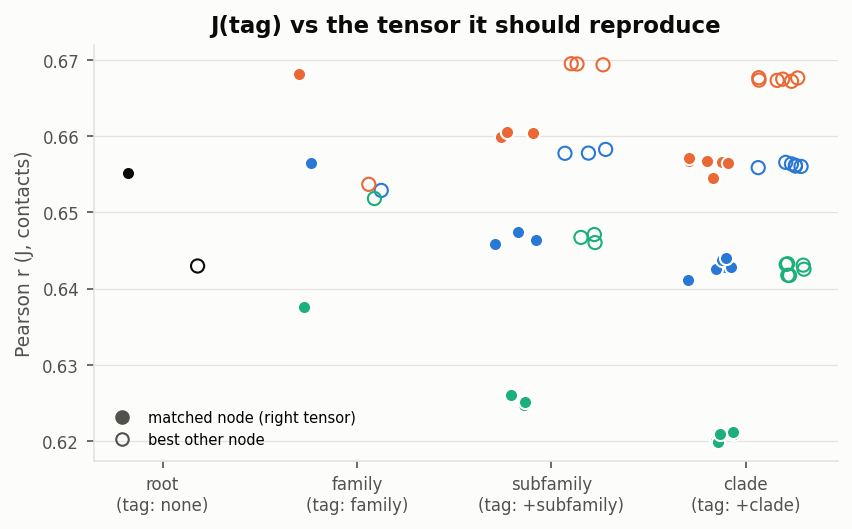
\includegraphics[width=0.55\linewidth]{models/fa_conditional_H128/tree_matched_rJ.png}
\caption{For each tag: $r_J$ with the tensor it should reproduce (filled) and with the best \emph{other} tensor
(open). At the family level the matched tensor wins for F0 and F1. At the subfamily and clade levels, another
tensor (always the tag's own family, or the root) correlates slightly better than the matched one.}
\end{figure}

By $r_J$, the true tensor that best matches each tag's $J$ is:
\begin{center}\small
\begin{tabular}{lcccc}
\toprule
level of the tag & itself & its own family & the root & another family\\
\midrule
family (3) & 2 & -- & 1 & 0\\
subfamily (9) & 0 & 6 & 3 & 0\\
clade (18) & 0 & 12 & 6 & 0\\
\bottomrule
\end{tabular}
\end{center}

\paragraph{Reading.}
\begin{enumerate}
\item \textbf{The couplings resolve the family, not the subfamily or the clade.} No tag's $J$ ever best
matches another family, but below the family level $J(\text{tag})$ is essentially the family's $J$. The
label-specific part of the couplings is weak and gets weaker with depth: $r(\Delta J)=0.34\to0.21\to0.11$.
\item \textbf{The fields carry the finer labels.} $r(\Delta h)=0.58\to0.50\to0.33$, about twice
$r(\Delta J)$ at every level. This is how the clade tags still select the right clade (100\% assignment
accuracy): the clade-specific conservation is learned in $h$.
\item \textbf{Why are the label-specific couplings weak?} Two reasons, both predictable from the architecture.
  (i) \emph{Capacity}: the label changes $J$ only through $\sum_hA^h_{ij}\Delta V^h(\text{tag})$, with the
  \emph{shared} attention and $H=128$ value matrices. The true clade perturbations are independent random blocks
  on 179 contacts, so by the rank argument of \S\ref{sec:rank} at most 128 of the 179 independent directions
  can be represented. (ii) \emph{Signal}: the true clade perturbations are small ($\sigma_J^{(3)}=0.15$, against
  0.8 for the root). Each clade tag sees only 8000 sequences, and the label tables are penalised
  ($\lambda_{\text{label}}$). The flat validation curve after epoch 10 shows that the extra label parameters
  mostly fit noise beyond that point.
\item \textbf{All couplings are shrunk.} The matched slope is $0.40$--$0.46$, i.e.\ the couplings along the
true direction are less than half their true size (0.57 in the unconditioned model). Part of the correlation
structure is instead carried by sharper fields: the generated sequences are slightly too conserved (identity
0.36 vs 0.34). Contact precision is still 1.00 for every tag.
\end{enumerate}

\subsection{Unconditioned vs conditioned}
\begin{center}\small
\begin{tabular}{p{0.36\linewidth}p{0.2\linewidth}p{0.34\linewidth}}
\toprule
 & unconditioned & conditioned (tags)\\
\midrule
validation pseudo-NLL per site & 0.949 & 0.873\\
family shares of generated sequences & 22/12/66\% & chosen by the tag (33/33/33\% pooled; 98--99\% correct per family tag)\\
$r_C$ per clade (oracle 0.83) & -- (no clade control) & 0.76\\
$r_C$ pooled (oracle 0.994) & 0.895 & 0.954\\
generated clade closest to its own test clade & -- & 18/18\\
$J$ resolves & the ancestor (root) & the family\\
long-range contact precision & 1.00 & 1.00\\
\bottomrule
\end{tabular}
\end{center}

\begin{keybox}{Conditioned model with $H=128$}
\begin{itemize}[nosep]
\item[+] Tags work: a clade tag generates its clade (18/18), a family tag its family (98--99\%), and pooling
      the tags gives the right family proportions. This removes the main failure of the unconditioned model.
\item[+] Per clade, $r_C=0.76$: between the sibling-clade level (0.63) and the noise floor (0.83).
\item[--] The learned couplings resolve only the family; subfamily and clade differences are carried mainly by
      the fields. All couplings are shrunk to $\approx40\%$ of their true size, and correlations are 10\% too weak.
\item[--] Without a tag the family weights are still off (33/21/46\%): the same pseudo-likelihood blind spot.
\end{itemize}
Levers to try next: $H=256$ (removes the rank bound on the label-specific couplings), label-specific
attention (lets tags change \emph{where} the couplings sit, not only their values), a smaller
$\lambda_{\text{label}}$ or more sequences per clade.
\end{keybox}


% Distance-based evaluation of the generated sequences (definitions in section sec:distances).
% Numbers from evaluations/<run>/metrics.json ["distances"].

\section{Results: distances between generated and real sequences}\label{sec:res_dist}
All quantities are defined in \S\ref{sec:distances}. They were computed for the four trained models; this
section reports the two $H=128$ models, and the $H=256$ models are compared in \S\ref{sec:res_H256}.

\subsection{Novelty: distance to the nearest training sequence}
\begin{center}\small
\begin{tabular}{lcccc}
\toprule
 & mean $d_{NN}$ & copies of a & $W_1$ vs & mean $d_{NN}$\\
 & to train & train seq. & test & of test seqs\\
\midrule
oracle (fresh true samples) & 0.378 & 0\% & 0.001 & 0.378\\
unconditioned, $H=128$ & 0.398 & 0\% & 0.019 & 0.378\\
conditioned, $H=128$ (per clade, mean) & 0.370 & 0\% & 0.011 & 0.378\\
\bottomrule
\end{tabular}
\end{center}
\textbf{No model copies its training data.} Not one of the 36{,}000 generated sequences equals a training sequence.
A typical held-out real sequence differs from its closest training sequence at 37.8\% of its sites
($\approx23$ of 60). The generated sequences are about as novel: the conditioned model's are marginally
\emph{closer} to the training set (0.370, i.e.\ half a site less), consistent with their slight over-conservation.
The unconditioned model's are slightly \emph{farther} (0.398). Our interpretation: a single Potts model fitted
to the mixture produces some hybrid sequences that combine features of different clades, and such sequences are
far from every training sequence.

\begin{figure}[H]
\centering
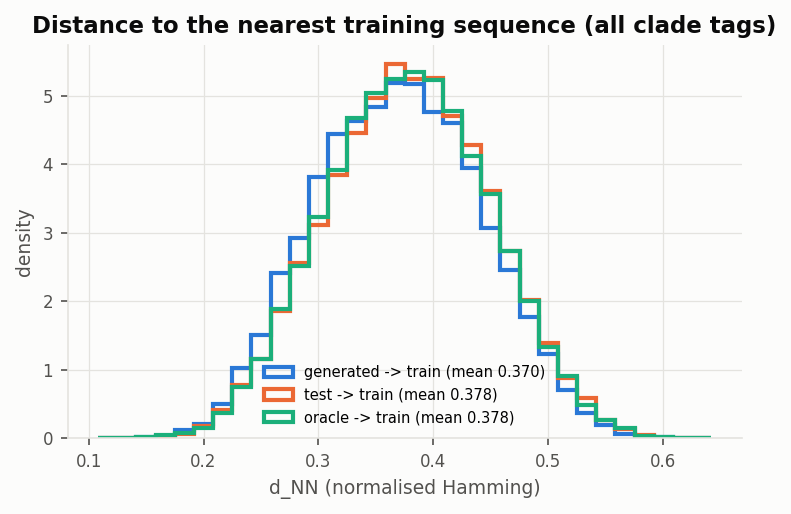
\includegraphics[width=0.49\linewidth]{models/fa_conditional_H128/dist_nn_to_train.png}\hfill
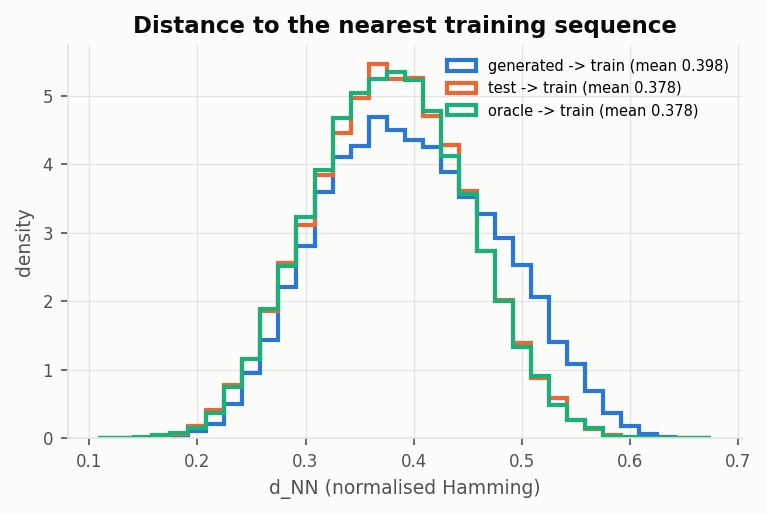
\includegraphics[width=0.49\linewidth]{models/fa_unconditional_H128/dist_nn_to_train.png}
\caption{Distribution of $d_{NN}$ to the training set. Left: conditioned model, all 18 clade tags. Right:
unconditioned model. Generated (blue), held-out test (orange), oracle (green). The oracle and test curves coincide
(same distribution); the generated curve of the conditioned model is shifted left by $\approx0.01$.}
\end{figure}

\subsection{Diversity: pairwise Hamming distances}
\begin{center}\footnotesize
\begin{tabular}{lccccc}
\toprule
 & $\bar D_{GG}$ & $\bar D_{RR}$ & $\bar D_{GR}$ & $W_1(D_{GG},D_{RR})$ & $W_1(D_{GR},D_{RR})$\\
 & (generated) & (test) & & &\\
\midrule
oracle, per clade (mean) & 0.664 & 0.663 & 0.664 & 0.003 & 0.002\\
conditioned $H=128$, per clade (mean) & 0.637 & 0.663 & 0.660 & 0.027 & 0.007\\
\midrule
oracle, pooled & 0.803 & 0.803 & 0.803 & 0.001 & 0.001\\
unconditioned $H=128$, pooled & 0.740 & 0.803 & 0.786 & 0.063 & 0.018\\
\bottomrule
\end{tabular}
\end{center}
\begin{itemize}
\item \textbf{Conditioned model.} Two sequences generated with the same clade tag differ at 63.7\% of the sites, against
66.3\% for two real sequences of that clade: 2.6\% (1.6 sites) less diversity. This is the same over-conservation
seen in the identity (0.36 vs 0.34). A generated--real pair, on the other hand, looks almost exactly like a
real--real pair ($W_1=0.007$).
\item \textbf{Unconditioned model.} The pooled diversity is clearly too low (0.740 vs 0.803). This is mostly the
wrong family weights: with 66\% of the samples in F2, most random pairs are same-family pairs, which are closer
(\S\ref{sec:res_props}).
\end{itemize}

\begin{figure}[H]
\centering
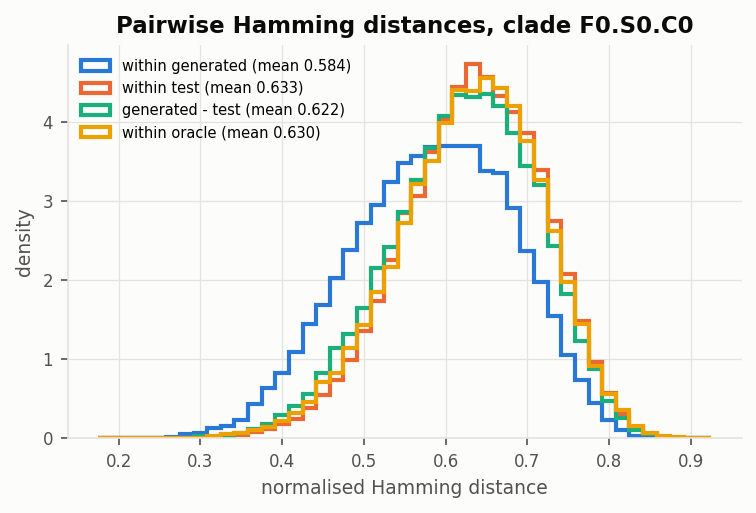
\includegraphics[width=0.49\linewidth]{models/fa_conditional_H128/dist_pairwise_F0.S0.C0.png}\hfill
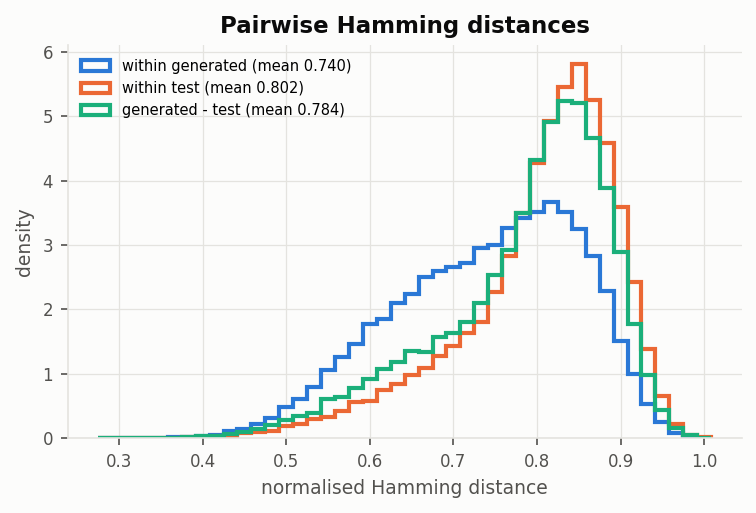
\includegraphics[width=0.49\linewidth]{models/fa_unconditional_H128/dist_pairwise.png}
\caption{Pairwise Hamming distance distributions. Left: clade \texttt{F0.S0.C0} with its tag (within generated, within
test, generated--test, within oracle). Right: unconditioned model, pooled over all clades.}
\end{figure}

\subsection{Position in PCA space: Fréchet distance}
The ladder built from the ground truth (\S\ref{sec:distances}), the Fréchet distance between the test sequences of
two clades, is
\begin{center}\small
\begin{tabular}{lcccc}
\toprule
 & same clade (oracle) & sibling clade & same family, other subfamily & other family\\
\midrule
FD (mean) & 0.02 & 1.48 & 6.15 & 21.4\\
\bottomrule
\end{tabular}
\end{center}
It spans three orders of magnitude, which makes it a sharp tool for placing a generated set in the hierarchy.
\begin{itemize}
\item \textbf{Conditioned $H=128$}: the generated clade vs its own test clade has FD $=0.39$ on average
(range 0.07--1.06). That is between the oracle (0.02) and the sibling clade (1.48). Even the worst generated clade (1.06) is closer
to its own test set than the average true sibling clade (1.48). For 17 of 18 generated clades the closest test clade
is their own (FD assignment accuracy 94\%; the $r_C$ assignment gave 18/18).
\item \textbf{Unconditioned $H=128$}, pooled: FD $=2.23$ against 0.001 for the oracle. The cloud is misplaced as a
whole because of the family weights.
\end{itemize}

\begin{figure}[H]
\centering
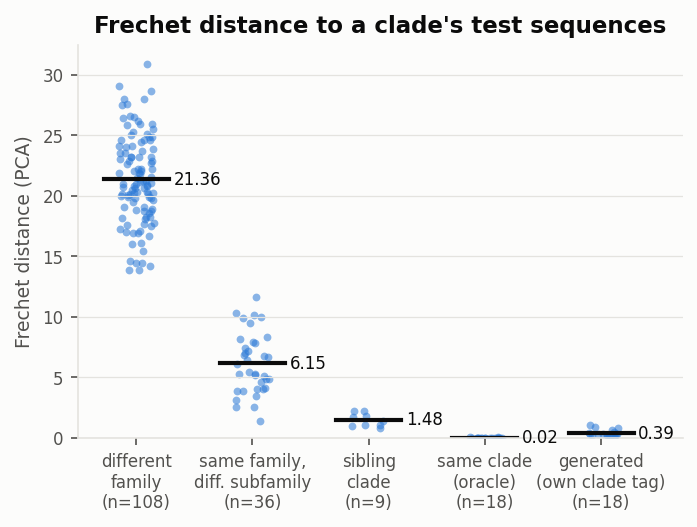
\includegraphics[width=0.49\linewidth]{models/fa_conditional_H128/frechet_ladder.png}\hfill
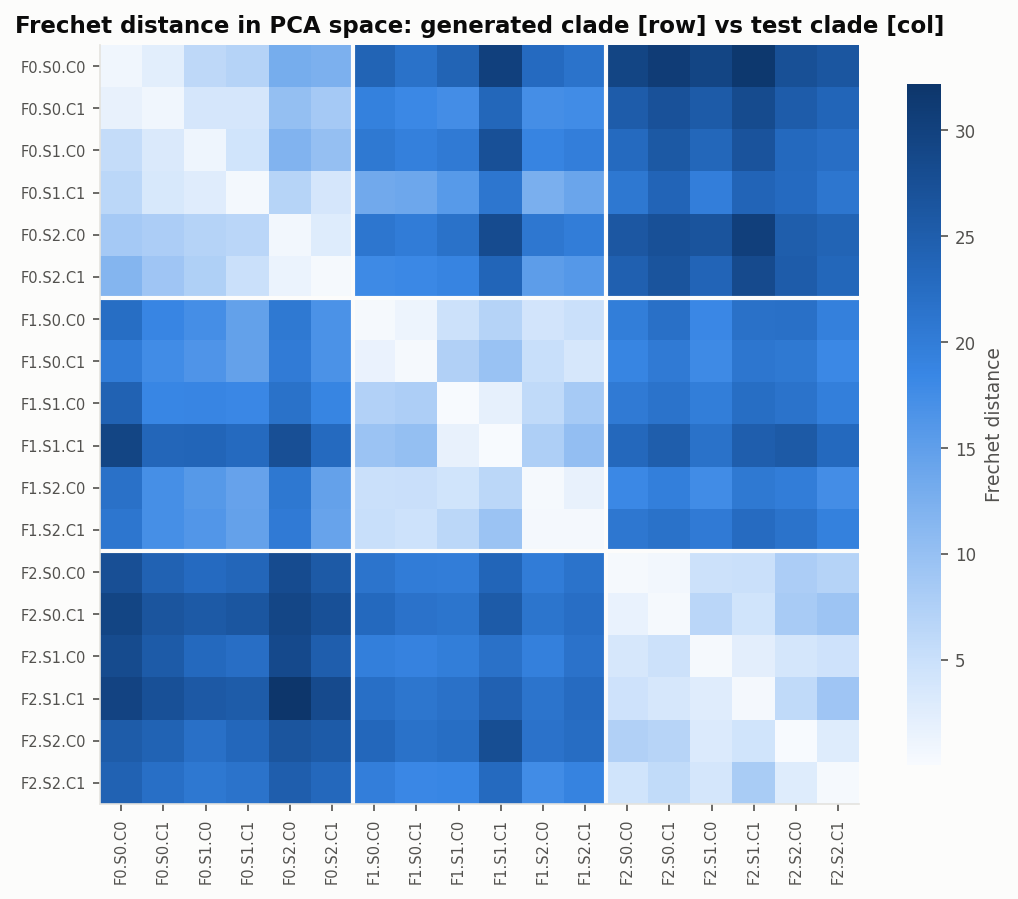
\includegraphics[width=0.49\linewidth]{models/fa_conditional_H128/cross_clade_frechet.png}
\caption{Left: FD to a clade's test sequences, for test sets of other clades grouped by relation (the ground-truth
ladder) and for the sequences generated with the clade's own tag (right-most column). Right: FD between each
generated clade (row) and each test clade (column); the dark diagonal and the family blocks are the hierarchy.}
\end{figure}

\begin{keybox}{What the distances add}
The three distance families agree with the statistics of \S\ref{sec:res_cond} and add two things:
(i) \textbf{no memorisation} (no copies, novelty equal to that of real held-out sequences); and
(ii) a \textbf{direct position in the hierarchy}: a generated clade is about 4 times closer to its own clade than
the sibling clade is (FD 0.39 vs 1.48), but 20 times farther than a perfect generator would be (0.02). Its
remaining defect is a small loss of diversity (1.6 sites), the sequence-level signature of fields that are too sharp.
\end{keybox}


% H = 128 vs H = 256 for both models.
% Numbers from evaluations/fa_{unconditional,conditional}_H{128,256}/{metrics,tree_comparison,mode_mixing}.json

\section{Results: more heads, $H=256$}\label{sec:res_H256}
Both models were retrained with $H=256$ heads, the value suggested by the rank argument of \S\ref{sec:rank}
($H\ge179$). All other settings were identical (configs \texttt{fa\_unconditional\_H256.json},
\texttt{fa\_conditional\_H256.json}; runs \texttt{fa\_*\_H256}).

\subsection{Summary table}
\begin{center}\footnotesize
\begin{tabular}{lcccc}
\toprule
 & \multicolumn{2}{c}{unconditioned} & \multicolumn{2}{c}{conditioned}\\
 & $H=128$ & $H=256$ & $H=128$ & $H=256$\\
\midrule
parameters & 0.54\,M & 1.09\,M & 2.12\,M & 4.19\,M\\
best epoch (stopped at) & 57 (60) & 36 (45) & 38 (47) & 10 (18)\\
validation pseudo-NLL / site & 0.949 & \textbf{0.946} & \textbf{0.873} & 0.888\\
\midrule
\multicolumn{5}{l}{\emph{parameters vs the ground truth (contact entries, zero-sum gauge)}}\\
$r_J$ (vs average of clades / matched clade) & 0.691 & \textbf{0.771} & 0.640 & \textbf{0.664}\\
slope of $J$ & 0.57 & \textbf{0.62} & \textbf{0.40} & 0.37\\
$r_h$ & \textbf{0.922} & 0.898 & \textbf{0.871} & 0.791\\
$r(\Delta J)$ family / subfamily / clade & -- & -- & 0.34/0.21/0.11 & 0.38/0.24/0.12\\
$r(\Delta h)$ family / subfamily / clade & -- & -- & 0.58/0.50/0.33 & 0.51/0.42/0.26\\
long-range contact precision & 1.00 & 1.00 & 1.00 & 1.00\\
\midrule
\multicolumn{5}{l}{\emph{generated sequences vs held-out test sequences}}\\
family shares (no tag) & 22/12/66\% & 11/13/76\% & 33/21/46\% & \textbf{28/31/41\%}\\
pooled $r_C$ (oracle 0.994) & \textbf{0.895} & 0.855 & \textbf{0.954} & 0.919\\
pooled $r_C$ after rebalancing & 0.949 & \textbf{0.952} & -- & --\\
per-clade $r_C$ (oracle 0.83) & -- & -- & \textbf{0.758} & 0.704\\
family-tag $r_C$ (mean) & -- & -- & 0.849 & \textbf{0.865}\\
per-clade FD in PCA space (oracle 0.02) & -- & -- & \textbf{0.39} & 0.62\\
FD assignment accuracy & -- & -- & \textbf{17/18} & 16/18\\
pairwise $\bar D_{GG}$ (test value) & 0.740 (0.803) & 0.716 (0.803) & 0.637 (0.663) & 0.633 (0.663)\\
mean $d_{NN}$ to train (test value 0.378) & 0.398 & 0.384 & 0.370 & 0.374\\
copies of training sequences & 0 & 0 & 0 & 0\\
\bottomrule
\end{tabular}
\end{center}

\subsection{Unconditioned model: better couplings, worse family weights}
With $H=256$ the learned couplings get closer to the truth ($r_J$ with the average of the clades $0.69\to0.77$,
slope $0.57\to0.62$; with the root $0.65\to0.73$). The statistics \emph{inside} each family improve (rebalanced
pooled $r_C$ 0.949 $\to$ 0.952). But the family weights get \emph{worse}: 11/13/76\% instead of 22/12/66\%. So the
pooled statistics, which include the weights, degrade ($r_C$ $0.895\to0.855$). The mixing check (\texttt{s08})
confirms again that this is the learned distribution, not the sampler: all starts converge to $\approx10/12/78\%$.
The energy/entropy decomposition \eqref{eq:freeenergy} gives an energy advantage of 13.3--13.5 for F2, compensated
by an entropy deficit of 11.6--11.8, a residual of $\approx1.8$ nats instead of 1.1--1.6.

This is a clean illustration of the pseudo-likelihood blind spot: \textbf{more capacity improves exactly what PL
measures} (each site given the others, $J$ and within-family statistics) \textbf{and does nothing for what PL
cannot see} (the relative weights of the families). A small, uncontrolled drift of the energy/entropy balance then
moves the weights further away.

\begin{figure}[H]
\centering
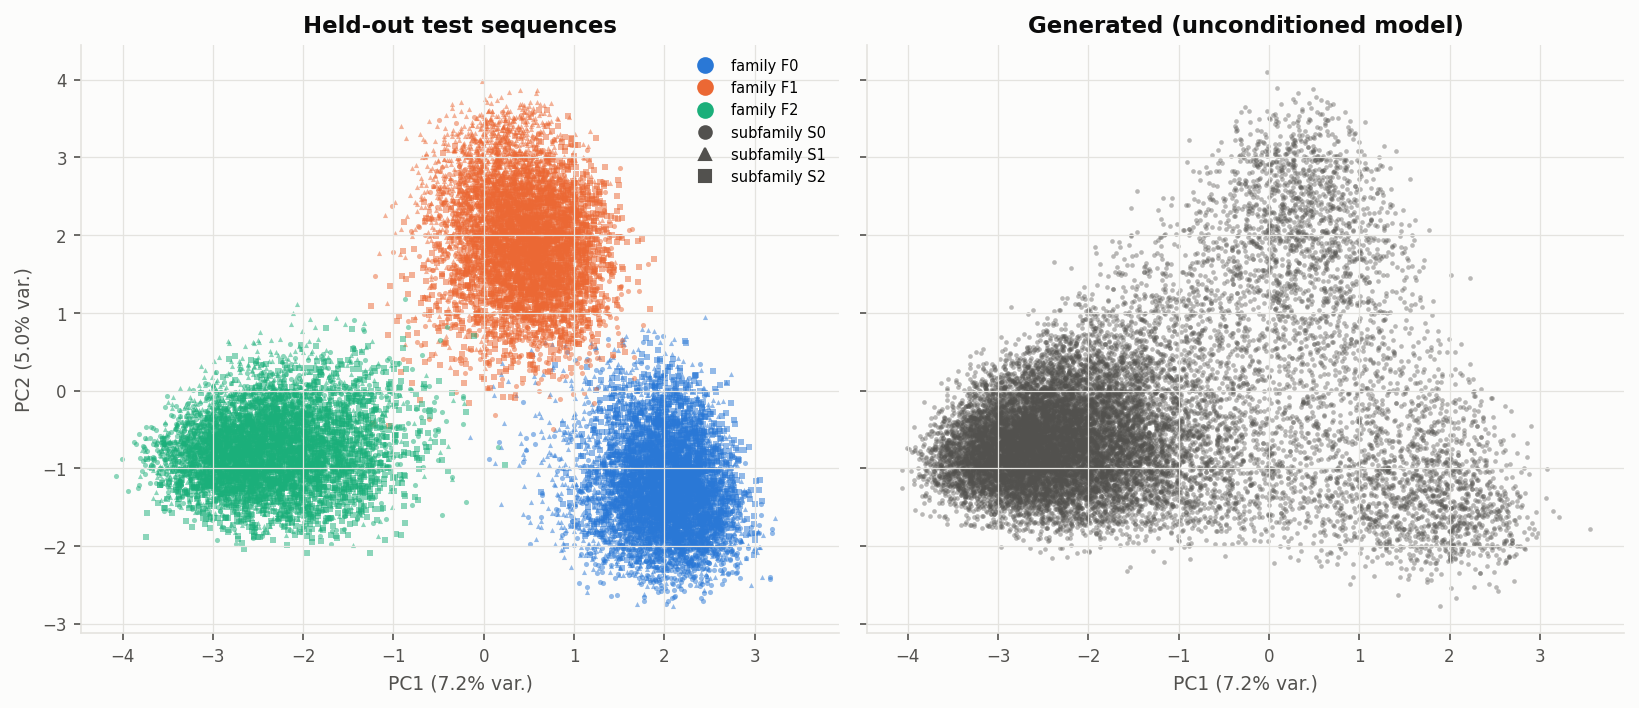
\includegraphics[width=0.85\linewidth]{models/fa_unconditional_H256/pca_generated_vs_test.png}
\caption{Unconditioned model with $H=256$: generated sequences on the reference PCA (right). F2 (bottom left) now
holds 76\% of the samples.}
\end{figure}

\subsection{Conditioned model: more heads did not help here}
The conditioned model with $H=256$ is \emph{worse} on most sequence metrics (per-clade $r_C$ $0.76\to0.70$, FD
$0.39\to0.62$), although its couplings are slightly better ($r_J$ $0.64\to0.66$, $r(\Delta J)$ slightly up at every
level). The reason is visible in the training curve. The validation loss is best at epoch 10 and does not improve afterwards, so
early stopping ended training at epoch 18. With twice the heads, the label tables hold twice as many parameters
(3.1\,M instead of 1.6\,M) under the same penalty $\lambda_{\text{label}}$. They start fitting noise within a few
epochs, before the fields have converged. The fields are indeed the component that got worse ($r_h$ $0.87\to0.79$,
$r(\Delta h)$ down at every level), and the fields are what carries the clade identity (\S\ref{sec:res_cond}).
Family-level behaviour, by contrast, improved: family tags are slightly better ($r_C$ 0.849 $\to$ 0.865) and the
no-tag family weights are closer to uniform (28/31/41\%). The mixing check confirms these weights (all starts
converge to $\approx28/31/41\%$), and the energy/entropy residual shrinks to 0.2--0.4 nats (energy terms $-9.1$ and
$-9.6$, entropy terms $+8.7$ and $+9.4$ for F0 and F1 relative to F2).

\begin{figure}[H]
\centering
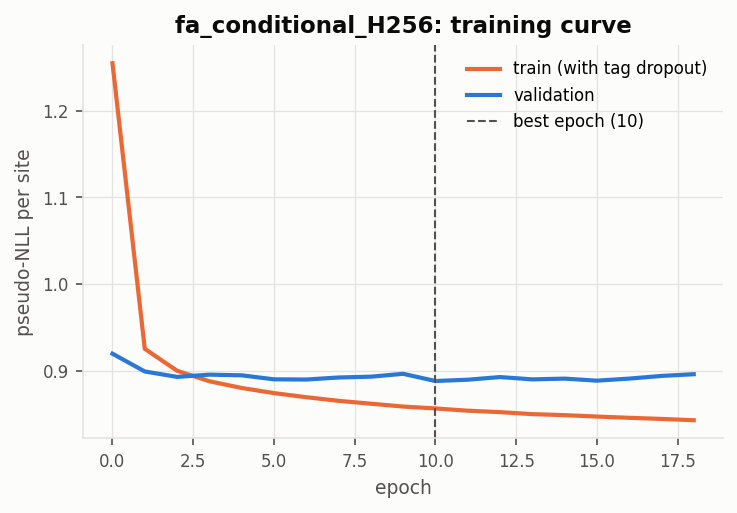
\includegraphics[width=0.49\linewidth]{models/fa_conditional_H256/training_curve.png}\hfill
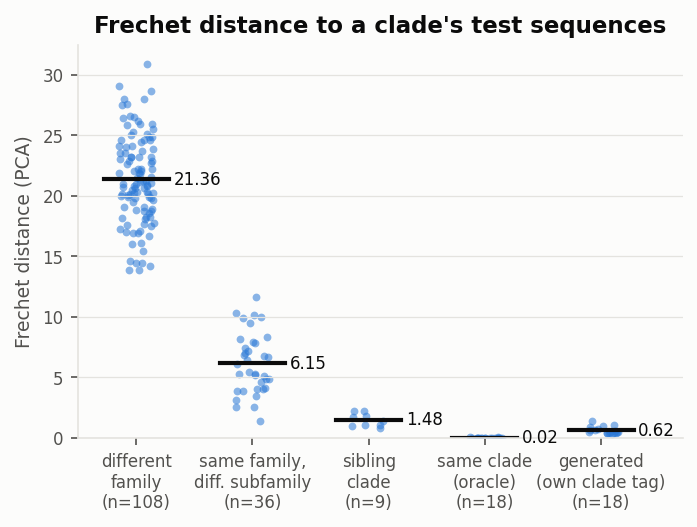
\includegraphics[width=0.49\linewidth]{models/fa_conditional_H256/frechet_ladder.png}
\caption{Conditioned model with $H=256$. Left: training curve (best epoch 10; compare the $H=128$ curve, best epoch 38).
Right: FD ladder; the generated clades (right-most column, mean 0.62) sit farther from their own clade than at
$H=128$ (0.39), still below the sibling clade (1.48).}
\end{figure}

\begin{keybox}{Conclusion on $H$}
\begin{itemize}[nosep]
\item $H=256$ recovers the couplings better in both models, as the rank argument predicts.
\item For the unconditioned model this does not translate into better samples, because its main error (family
      weights) is invisible to pseudo-likelihood and got worse.
\item For the conditioned model, the doubled label tables over-fit quickly with the current
      $\lambda_{\text{label}}=10^{-4}$, and early stopping cuts training before the fields are learned.
      $H=256$ therefore needs a stronger label penalty (or a smaller learning rate / more data per clade). As it
      stands, \textbf{the best generator is still the conditioned model with $H=128$}.
\end{itemize}
\end{keybox}


%------------------------------------------------------------------------------------------
\section{Training plan}\label{sec:plan}
%------------------------------------------------------------------------------------------
% Training plan.
\paragraph{Status.} The unconditioned model has been trained, with $H=128$ instead of 256 at your request
(results in \S\ref{sec:res_uncond}). The conditioned model has been trained with $H=128$ as well
(results in \S\ref{sec:res_cond}). Both were then retrained with $H=256$ (\S\ref{sec:res_H256}), and all four
runs were evaluated with the distance metrics of \S\ref{sec:distances} (\S\ref{sec:res_dist}).

\paragraph{Commands} (in order; all have been run, for $H=128$ and for $H=256$ with the \texttt{*\_H256.json} configs):
{\small\begin{verbatim}
python scripts/s04_make_dataset.py              # done: 144k / 18k / 18k
python scripts/s05_train_factored_attention.py --config configs/fa_unconditional.json
python scripts/s05_train_factored_attention.py --config configs/fa_conditional.json
python scripts/s06_evaluate_model.py --config configs/fa_unconditional.json
python scripts/s06_evaluate_model.py --config configs/fa_conditional.json
python scripts/s07_compare_to_tree.py --config <run config>   # J vs every tree J
python scripts/s08_mode_mixing.py --config <run config>       # model or sampler?
\end{verbatim}}

\paragraph{Hyper-parameters} (\texttt{configs/fa\_unconditional.json}, \texttt{configs/fa\_conditional.json}):
\begin{center}\small
\begin{tabular}{p{0.2\linewidth}p{0.3\linewidth}p{0.4\linewidth}}
\toprule
 & unconditioned & conditioned\\
\midrule
heads $H$, key dim $d$ & 256, 32 & 256, 32\\
parameters & 1{,}086{,}640 & 4{,}194{,}640\\
training data & all 18 clades, no tags & all 18 clades, tags with hierarchical dropout (0.10/0.10/0.15)\\
loss & PL \eqref{eq:pl} $+10^{-5}(\|h\|^2+\|J\|^2)$ & same $+\,10^{-4}\sum(\|\Delta h\|^2+\|\Delta J\|^2)$\\
optimiser & Adam, lr $5\times10^{-3}$, batch 512 & same\\
epochs & $\le60$, early stopping (patience 8) on val.\ PL & same\\
\bottomrule
\end{tabular}
\end{center}

\paragraph{Cost} (measured with 40 optimiser steps on the real data, NVIDIA RTX 2060): about
$0.2$\,min per epoch (unconditioned) and $0.4$\,min per epoch (conditioned), under 0.3\,GB of GPU memory.
That is at most $\approx12$ and $\approx25$ minutes for 60 epochs. Evaluation (Gibbs sampling of 18{,}000
sequences per model plus the oracle samples) takes a few minutes.

\paragraph{Reference values for the validation pseudo-NLL per site} (computed on the validation set):
\begin{center}\small
\begin{tabular}{lc}
\toprule
model & pseudo-NLL per site\\
\midrule
uniform residues (knows nothing) & $\log 20 = 3.00$\\
independent sites, one profile $f_i$ for all clades & 2.11\\
independent sites, one profile per clade & 1.63\\
\textbf{true clade Potts models} (the floor for the conditioned model with full tags) & \textbf{0.80}\\
\bottomrule
\end{tabular}
\end{center}
After only 40 steps the models are at 1.80 (unconditioned) and 1.53 (conditioned). The unconditioned model
cannot reach 0.80, because a single Potts model cannot represent the 18-clade mixture (\S\ref{sec:cond}). How
close it gets is itself a result.

\paragraph{What we will look at after training} (all produced by \texttt{s06}):
\begin{enumerate}[nosep]
\item training curves (\texttt{figures/models/<run>/training\_curve.png});
\item per clade: generated $r_C$ vs the oracle $r_C$ ($\approx0.83$), \texttt{rC\_per\_clade.png};
\item the cross-clade $r_C$ matrix and assignment accuracy: does the clade tag really select the clade
      rather than only its family? Compare with the reference ladder 0.83 / 0.63 / 0.35 / 0.08 of \S\ref{sec:refvalues};
\item $J$ recovery ($r_J$ on contacts) and contact precision, per clade;
\item PCA of generated vs test sequences;
\item unconditioned vs conditioned: what conditioning buys.
\end{enumerate}

\begin{checkbox}{Points to confirm before launching}
\begin{enumerate}[nosep]
\item The index reading of your formula, eq.~\eqref{eq:falogit}, together with the self-mask and the symmetrisation \eqref{eq:sym2}.
\item $H=256$ heads, from the rank argument of \S\ref{sec:rank}. Fewer heads would test whether the model can
      compress the couplings; our random ground truth predicts it cannot below $\approx179$.
\item Shared attention with label-specific values/fields in the conditioned model (\S\ref{sec:cond}). The
      alternative, label-specific $Q,K$, would let clades have different contact maps, which our ground truth does not have.
\end{enumerate}
\end{checkbox}



% ==========================================================================================
% PART III : masked (absorbing-state) discrete diffusion
% ==========================================================================================
\part{A masked diffusion model}

\section{Idea: learn to un-mask}\label{sec:md_idea}
The Potts models of Part~II had to write the distribution in a fixed form, $e^{-E(\s)}/Z$, and were trained by
pseudo-likelihood, which never sees $Z$. We saw what that costs: wrong family weights. A diffusion model takes a
different route. It never writes $P(\s)$ explicitly. Instead it learns to \emph{undo a corruption}:
\begin{enumerate}[nosep]
\item \textbf{Forward (corruption)}: take a real sequence and hide more and more of its residues behind a special
      symbol \texttt{[M]} (``mask''), until everything is hidden.
\item \textbf{Reverse (generation)}: a neural network, the \emph{denoiser}, looks at a partially hidden sequence and
      says, for every hidden site, how likely each amino acid is. Starting from a fully hidden sequence and revealing
      sites one after another with these probabilities generates a new sequence.
\end{enumerate}
Because \texttt{[M]} is a state the forward process can enter but never leave, this is called
\emph{absorbing-state} (or \emph{masked}) diffusion. We follow the MDLM formulation (Sahoo et al., 2024). The network
outputs probabilities directly and no couplings are involved. The training loss is a bound on the true
log-likelihood $-\log p_\theta(\s)$, which, unlike the pseudo-likelihood, includes the global normalisation.

\section{The forward process}\label{sec:md_forward}
Extend the alphabet with one symbol, \texttt{[M]} (index $q=20$). A \emph{noise level} $t\in[0,1]$ sets how much is
hidden through a decreasing function $\alpha_t$ with $\alpha_0=1$, $\alpha_1=0$. We use the linear schedule
$\alpha_t=1-t$. Each site is corrupted \emph{independently}:
\begin{equation}\label{eq:md_forward}
q(x^i_t\mid x^i_0)=\alpha_t\,\one[x^i_t=x^i_0]+(1-\alpha_t)\,\one[x^i_t=\texttt{[M]}],\qquad
q(\bm x_t\mid\bm x_0)=\prod_{i=1}^Lq(x^i_t\mid x^i_0).
\end{equation}
At time $t$ each site is still visible with probability $\alpha_t=1-t$ and hidden with probability $t$; at $t=1$
everything is hidden. \texttt{test\_13} checks that the fraction of masked sites equals $t$ and that visible sites are untouched.

\paragraph{From $s$ to $t$ ($s<t$).} A site visible at $s$ must stay visible until $t$. Since $\alpha_t=\alpha_s\cdot(\alpha_t/\alpha_s)$,
the process is a Markov chain in which a visible site survives from $s$ to $t$ with probability $\alpha_t/\alpha_s$ and a
masked site stays masked forever:
\[
q(x^i_t\mid x^i_s)=\begin{cases}\alpha_t/\alpha_s & x^i_t=x^i_s\neq\texttt{[M]}\\ 1-\alpha_t/\alpha_s & x^i_t=\texttt{[M]},\ x^i_s\neq\texttt{[M]}\\ 1 & x^i_t=x^i_s=\texttt{[M]}.\end{cases}
\]
Equivalently, every site is hidden at an independent random time, uniformly distributed on $[0,1]$ for the
linear schedule. We use this picture for the sampler.

\section{The reverse process}\label{sec:md_reverse}
\subsection{If we knew the clean sequence: the exact posterior}
Consider one site that is hidden at time $t$. What was it at an earlier time $s<t$? By Bayes' rule,
$q(x^i_s\mid x^i_t,x^i_0)\propto q(x^i_t\mid x^i_s)\,q(x^i_s\mid x^i_0)$. Given $x^i_t=\texttt{[M]}$, there are only two
possibilities for $x^i_s$:
\begin{itemize}[nosep]
\item $x^i_s=\texttt{[M]}$: weight $1\cdot(1-\alpha_s)$;
\item $x^i_s=x^i_0$ (visible at $s$, hidden between $s$ and $t$): weight $(1-\alpha_t/\alpha_s)\cdot\alpha_s=\alpha_s-\alpha_t$.
\end{itemize}
The two weights sum to $1-\alpha_t$, so
\begin{equation}\label{eq:md_posterior}
\boxed{\;q(x^i_s\mid x^i_t=\texttt{[M]},x^i_0)=\frac{1-\alpha_s}{1-\alpha_t}\,\one[x^i_s=\texttt{[M]}]
+\frac{\alpha_s-\alpha_t}{1-\alpha_t}\,\one[x^i_s=x^i_0]\;}
\end{equation}
and a visible site simply stays: $q(x^i_s\mid x^i_t\neq\texttt{[M]})=\one[x^i_s=x^i_t]$. For the linear schedule the
probability of being revealed between $t$ and $s$ is $\frac{\alpha_s-\alpha_t}{1-\alpha_t}=\frac{t-s}{t}$.

\subsection{The model: replace the unknown $x_0$ by the denoiser}
At generation time $x^i_0$ is unknown. The model keeps the form \eqref{eq:md_posterior} and replaces the indicator
$\one[x^i_s=x^i_0]$ by the network's guess:
\begin{equation}\label{eq:md_model}
p_\theta(x^i_s\mid\bm x_t)=\frac{1-\alpha_s}{1-\alpha_t}\,\one[x^i_s=\texttt{[M]}]+\frac{\alpha_s-\alpha_t}{1-\alpha_t}\,
\underbrace{p_\theta(x^i_0=x^i_s\mid\bm x_t,t)}_{\text{denoiser}}\qquad(x^i_t=\texttt{[M]}),
\end{equation}
where the \textbf{denoiser} $p_\theta(x^i_0=a\mid\bm x_t,t)$ is a probability distribution over the 20 amino acids
for every hidden site, computed by a neural network that sees the whole partially hidden sequence. Two
constraints are built in (the ``SUBS'' parametrisation): the denoiser puts no probability on \texttt{[M]} (its
output layer has 20 entries), and visible sites are never changed.

\subsection{What should the denoiser output? The optimal denoiser}\label{sec:md_optimal}
Suppose the network could be anything. For a given $\bm x_t$, the best answer is the true conditional probability
of the clean residue given everything that is visible. By Bayes' rule and \eqref{eq:md_forward},
\[
p(\bm x_0\mid\bm x_t)\propto p(\bm x_0)\,q(\bm x_t\mid\bm x_0)
=p(\bm x_0)\,\alpha_t^{\#\text{visible}}(1-\alpha_t)^{\#\text{hidden}}\;\one[\bm x_0\text{ agrees with }\bm x_t\text{ on the visible sites}].
\]
The factor $\alpha_t^{\#\text{visible}}(1-\alpha_t)^{\#\text{hidden}}$ is the same for every $\bm x_0$ compatible with
$\bm x_t$, so it cancels in the normalisation:
\begin{equation}\label{eq:md_opt}
\boxed{\;p^\star(x^i_0=a\mid\bm x_t,t)=P\big(x^i=a\ \big|\ \text{the visible sites of }\bm x_t\big)\;}
\end{equation}
It \textbf{does not depend on $t$}: the masking is independent of the residues, so the noise level carries no
information about them. (We nevertheless give $t$ to the network, as you chose. This is the classic design, and
it lets us check empirically that the network learns to ignore it.) Two special cases connect with the rest of
this document:
\begin{itemize}[nosep]
\item everything hidden: $p^\star(x^i_0=a\mid\texttt{[M]}\dots\texttt{[M]})=f_i(a)$, the single-site frequencies;
\item only site $i$ hidden: $p^\star=P(x^i=a\mid\bm x_{-i})$, exactly the conditional that the pseudo-likelihood of
      Part~II fits. For our data it is the Potts conditional \eqref{eq:cond} of the clade the sequence came from.
\end{itemize}
So the network \textbf{directly outputs probabilities}. \texttt{test\_14} verifies both special cases on a tiny Potts model
where the exact answers are known, and \texttt{s10} measures the second one on the real test sequences.

\section{The loss: a bound on the likelihood}\label{sec:md_elbo}
\subsection{From the ELBO to a weighted cross-entropy}
Divide $[0,1]$ into $T$ steps $t_k=k/T$. The standard variational bound of a diffusion model (the evidence lower
bound, ELBO) reads
\begin{align*}
-\log p_\theta(\bm x_0)\le{}&\underbrace{\mathrm{KL}\big(q(\bm x_1|\bm x_0)\,\|\,p(\bm x_1)\big)}_{=0}
+\underbrace{(\text{reconstruction at }t=0)}_{=0}\\
&+\sum_{k=1}^{T}\E_{q(\bm x_{t_k}|\bm x_0)}\Big[\mathrm{KL}\big(q(\bm x_{t_{k-1}}|\bm x_{t_k},\bm x_0)\,\|\,p_\theta(\bm x_{t_{k-1}}|\bm x_{t_k})\big)\Big].
\end{align*}
(The derivation is the usual one: write $\log p_\theta(\bm x_0)=\log\E_q[p_\theta(\bm x_{0:1})/q(\bm x_{t_1:1}\mid\bm x_0)]$ and
apply Jensen's inequality $\log\E\ge\E\log$.) The first term vanishes because at $t=1$ everything is masked for
both $q$ and the model. The last vanishes because at $t=0$ nothing is masked. Each KL is a sum over sites (the
site-wise factorisation of \eqref{eq:md_posterior}, \eqref{eq:md_model}). For a site visible at $t$ both
distributions are the same point mass, so KL $=0$. For a hidden site, both put the \emph{same} mass
$\frac{1-\alpha_s}{1-\alpha_t}$ on \texttt{[M]}; $q$ puts the rest on $x^i_0$, and the model spreads it as
$\frac{\alpha_s-\alpha_t}{1-\alpha_t}\,p_\theta(\cdot\mid\bm x_t)$. Hence
\begin{align*}
\mathrm{KL}&=\frac{1-\alpha_s}{1-\alpha_t}\underbrace{\log\frac{(1-\alpha_s)/(1-\alpha_t)}{(1-\alpha_s)/(1-\alpha_t)}}_{=0}
+\frac{\alpha_s-\alpha_t}{1-\alpha_t}\log\frac{(\alpha_s-\alpha_t)/(1-\alpha_t)}{\big[(\alpha_s-\alpha_t)/(1-\alpha_t)\big]\,p_\theta(x^i_0\mid\bm x_t)}\\
&=\frac{\alpha_s-\alpha_t}{1-\alpha_t}\,\big(-\log p_\theta(x^i_0\mid\bm x_t)\big).
\end{align*}
Summing over the $T$ steps and letting $T\to\infty$, $\alpha_{t_{k-1}}-\alpha_{t_k}\to-\alpha'_t\,dt$ and the sum becomes an
integral:
\begin{equation}\label{eq:md_nelbo}
-\log p_\theta(\bm x_0)\le\mathcal L_{\text{NELBO}}(\bm x_0)=\int_0^1\frac{-\alpha'_t}{1-\alpha_t}\;
\E_{\bm x_t\sim q(\cdot|\bm x_0)}\Big[\sum_{i:\,x^i_t=\texttt{[M]}}-\log p_\theta(x^i_0\mid\bm x_t,t)\Big]dt ,
\end{equation}
and for the linear schedule ($-\alpha'_t=1$, $1-\alpha_t=t$):
\begin{equation}\label{eq:md_nelbo_lin}
\boxed{\;\mathcal L_{\text{NELBO}}(\bm x_0)=\E_{t\sim\mathcal U(0,1)}\,\E_{\bm x_t}\Big[\frac1t\sum_{i\text{ hidden}}-\log p_\theta(x^i_0\mid\bm x_t,t)\Big]\;}
\end{equation}
In words: \textbf{hide a random fraction $t$ of the sites, ask the network to predict the hidden residues, and
average the cross-entropy with weight $1/t$}. The weight compensates for the number of hidden sites, $\approx tL$,
so that every noise level contributes comparably. We report $\mathcal L_{\text{NELBO}}/L$ in nats per site. It is an
\emph{upper bound} on $-\log p_\theta(\bm x)/L$, the true negative log-likelihood per site. Unlike the pseudo-likelihood,
it therefore involves the full normalisation.

\subsection{Why the bound can be tight}
With the optimal denoiser \eqref{eq:md_opt}, the bound becomes an equality in expectation:
$\E\,\mathcal L_{\text{NELBO}}(\bm x)=-\log p(\bm x)$. The intuition goes through the sampler of \S\ref{sec:md_sampler}. It
reveals the sites in a uniformly random order $\sigma$ and draws each from the denoiser. With the exact conditionals,
every ordering reproduces $p(\bm x)$ through the chain rule,
$p(\bm x)=\prod_kP(x^{\sigma_k}\mid x^{\sigma_1},\dots,x^{\sigma_{k-1}})$, and the NELBO is the average over orderings of
$-\log$ of this product. \texttt{test\_13} checks numerically, on a tiny Potts model with an exact denoiser built by
enumeration, that the NELBO equals the entropy of the distribution.

\subsection{Practical details}
\begin{itemize}[nosep]
\item \textbf{Variance reduction}: within a batch of $B$ sequences the times are stratified, $t_b=(u+b/B)\bmod1$ with a
      single $u\sim\mathcal U(0,1)$, and clipped to $[10^{-3},1]$ (the $1/t$ weight is large near 0).
\item \textbf{Optimiser}: AdamW, learning rate $3\times10^{-4}$ with 1000 warm-up steps, gradient clipping at 1, batch 256,
      mixed precision (fp16 with gradient scaling, on the GPU's tensor cores).
\item \textbf{EMA}: we keep an exponential moving average of the weights, $\bar\theta\leftarrow0.999\,\bar\theta+0.001\,\theta$ after
      every step, and evaluate and save $\bar\theta$ (a standard stabiliser for diffusion models).
\item \textbf{Validation}: $\mathcal L_{\text{NELBO}}/L$ on the 18{,}000 validation sequences, with the \emph{same} random times and
      masks at every epoch (4 draws per sequence), for early stopping (patience 15, at most 150 epochs).
\end{itemize}

\section{Sampling}\label{sec:md_sampler}
\paragraph{Ancestral sampler with $T$ steps.} Start from $\bm x_1=\texttt{[M]}\cdots\texttt{[M]}$. For $t=1,1-\frac1T,\dots,\frac1T$ and
$s=t-\frac1T$: for every hidden site, reveal it with probability $\frac{t-s}{t}$ (eq.~\eqref{eq:md_posterior}), drawing
its residue from the denoiser $p_\theta(\cdot\mid\bm x_t,t)$. At the last step ($s=0$) every remaining site is revealed.
\textbf{Caveat}: sites revealed in the \emph{same} step are drawn \emph{independently} of each other, from the same $\bm x_t$. If two
correlated sites are revealed together, their correlation is lost. With $T=1$ all $L$ sites are drawn at once from
$p_\theta(\cdot\mid\text{all hidden})=f_i$: independent sites. The error disappears only when steps are so small that
sites are revealed one at a time. \texttt{test\_13} (figure below) shows this with the exact denoiser: the total-variation
error goes from the independent-sites value at $T=1$ to the sampling noise at $T\gtrsim30$ for $L=4$.

\paragraph{Exact continuous-time sampler.} The $T\to\infty$ limit can be simulated exactly. In the forward process
each site is hidden at an independent uniform time, so in reverse the sites are revealed one at a time, in a
uniformly random order, the $k$-th reveal occurring at the $k$-th largest of $L$ uniform times $\tau_{(1)}>\dots>\tau_{(L)}$.
The sampler draws those times, then for $k=1,\dots,L$ reveals the $k$-th site from $p_\theta(\cdot\mid\bm x_{\tau_{(k)}},\tau_{(k)})$.
That is \textbf{exactly $L=60$ network calls per sequence}, with no step-size error
(\texttt{continuous\_time\_sample}; \texttt{test\_13} checks that it reproduces the exact distribution). It is our main sampler.
The finite-$T$ sampler is kept to measure the step-size effect on real data ($T=15,60,240$).

\begin{figure}[H]
\centering
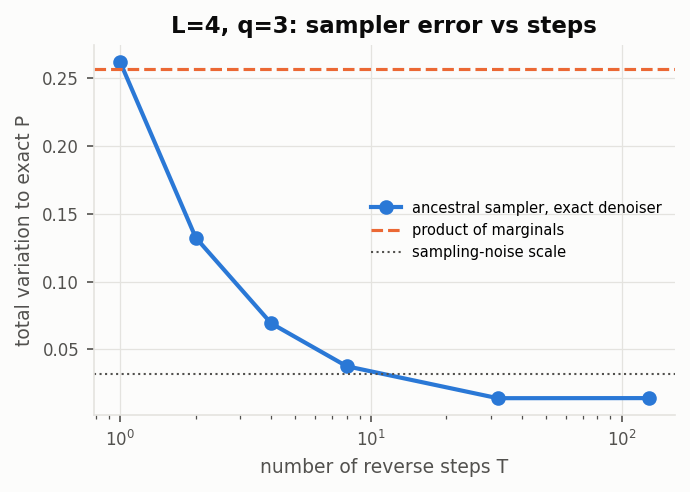
\includegraphics[width=0.48\linewidth]{tests/test_13_masked_diffusion/test_ancestral_sampler_with_exact_denoiser/tv_vs_steps.png}
\caption{\texttt{test\_13}: $L=4$, $q=3$ Potts model, exact denoiser. Distance of the ancestral sampler's output to the exact
distribution vs the number of steps $T$. $T=1$ gives the product of the marginals (independent sites); large $T$ is exact.}
\end{figure}

\section{The network}\label{sec:md_network}
The denoiser is a bidirectional transformer. Unlike the factored attention of Part~II, its attention weights
\emph{depend on the residues}, so it is not restricted to pairwise (Potts) interactions.
\begin{center}\footnotesize
\begin{tabular}{p{0.12\linewidth}p{0.5\linewidth}p{0.28\linewidth}}
\toprule
stage & operation & shape / parameters\\
\midrule
input & $\bm x_t\in\{0,\dots,19,\texttt{[M]}\}^{60}$, noise level $t\in[0,1]$ & $(B,60)$, $(B,)$\\
embedding & token emb.\ ($21\times256$) $+$ position emb.\ ($60\times256$) $+$ time emb. & $(B,60,256)$; 90{,}880 params\\
time emb. & $[\sin2\pi2^kt,\cos2\pi2^kt]_{k=0..7}\to$ Linear--GELU--Linear & (included above)\\
encoder & $6\times$[LayerNorm $\to$ self-attention (8 heads) $\to$ LayerNorm $\to$ MLP $256{\to}1024{\to}256$], with residual connections & 4{,}738{,}560 params\\
head & LayerNorm $\to$ Linear $256\to20$ & 5{,}652 params\\
output & logits of $p_\theta(x^i_0=a\mid\bm x_t,t)$ for every site & $(B,60,20)$\\
\midrule
total & & \textbf{4{,}835{,}092} parameters\\
\bottomrule
\end{tabular}
\end{center}
Each layer adds its input back (residual connections), so information can flow straight through. The LayerNorms
rescale the vectors to keep the training stable. Self-attention lets every site gather information from every
other site, with weights that depend on what is there.

\paragraph{Training data and cost.} The same 144{,}000 training sequences of all 18 clades, \textbf{without any label}
(unconditioned, as you chose), and the same validation and test splits as in Part~II. Measured on the RTX~2060:
74\,ms per step in mixed precision (181\,ms in fp32), i.e.\ $\approx45$\,s per epoch plus validation, so at most
$\approx2$\,h for 150 epochs.

\section{Tests of Part III}\label{sec:md_tests}
\begin{center}\small
\begin{tabular}{p{0.3\linewidth}p{0.62\linewidth}}
\toprule
test & what it verifies\\
\midrule
\texttt{test\_13\_masked\_diffusion} & masked fraction $=t$, visible sites untouched; stratified times; output shape (20 classes, no mass on
\texttt{[M]}); the output depends on $t$; save/load; \textbf{with the exact denoiser the NELBO equals the entropy}, and a uniform
denoiser gives $L\log q$; ancestral sampler: $T=1$ gives independent sites, large $T$ is exact; continuous-time sampler is
exact; one-site-masked readout $=$ the Potts conditional\\
\texttt{test\_14\_diffusion\_training} & a small denoiser trained on 20{,}000 samples of an $L=4$, $q=3$ Potts model (81 states):
validation NELBO within 0.03 nats/site of the exact $-\log p$ of the validation sequences; fully-masked output $=$ marginals;
one-site-masked output $=$ Potts conditionals (probability-weighted error $<0.03$); samples: total variation $0.028$ to the
exact distribution\\
\texttt{test\_15\_diffusion\_pipeline} & the whole chain (dataset $\to$ \texttt{s09} train $\to$ \texttt{s10} evaluate) on a tiny tree, with mixed precision\\
\texttt{test\_16\_checkpointing} & checkpoint files are written (best model, full state, snapshots every $N$ epochs); 4 epochs $+$ resume to 6 gives exactly the same losses and weights as 6 epochs in one go\\
\texttt{test\_10} (added case) & the pseudo-likelihood clade classifier of \texttt{s11} assigns samples of two Potts models to the right one; its score equals the sum of the log conditionals\\
\bottomrule
\end{tabular}
\end{center}

\begin{figure}[H]
\centering
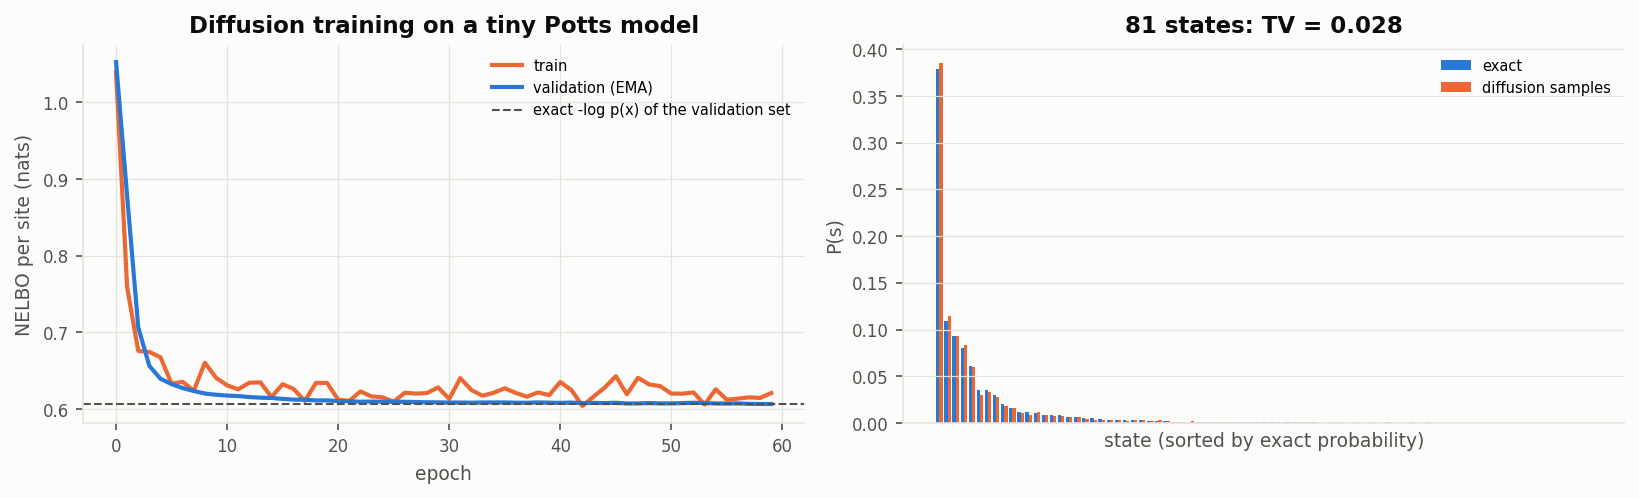
\includegraphics[width=\linewidth]{tests/test_14_diffusion_training/test_learns_tiny_potts/tiny_potts_diffusion.png}
\caption{\texttt{test\_14}. Left: training curve on the tiny Potts model; the dashed line is the exact $-\log p(\bm x)$ per site of the
validation sequences, which the bound approaches from above. Right: the 81 states, exact probability vs frequency in
20{,}000 diffusion samples.}
\end{figure}

\section{What we will measure}\label{sec:md_plan}
With the same held-out test set and the same metrics as the Potts models (\texttt{s10}):
\begin{enumerate}[nosep]
\item test NELBO per site (the likelihood bound);
\item \textbf{the probabilities themselves}: $p_\theta(x^i\mid\bm x_{-i})$ on test sequences vs the exact conditional of the true clade
      model, and the resulting pseudo-NLL per site, directly comparable with Part~II (true models 0.80, conditioned Potts
      0.873, unconditioned Potts 0.949);
\item samples: $r_f$, $r_C$, identity, \textbf{family proportions} (the main failure of the unconditioned Potts model; a likelihood
      bound should get them right), distances (novelty, diversity, Fréchet), for the continuous-time sampler and for $T=15,60,240$.
\end{enumerate}


% Masked diffusion: implementation, training and results.
% Numbers from models/md_unconditional/history.json, evaluations/md_unconditional/{metrics,time_dependence}.json,
% evaluations/comparison/summary.json

\section{Implementation}\label{sec:md_impl}
\begin{center}\footnotesize
\begin{tabular}{p{0.34\linewidth}p{0.58\linewidth}}
\toprule
file / function & role\\
\midrule
\texttt{psg/models/masked\_diffusion.py} & \\
\quad\texttt{mask\_tokens} & forward process \eqref{eq:md_forward}: each site masked independently with probability $t$\\
\quad\texttt{sample\_times} & stratified times $t_b=(u+b/B)\bmod1$, mapped to $[10^{-3},1]$\\
\quad\texttt{nelbo\_per\_sequence} & one-sample estimate of \eqref{eq:md_nelbo_lin}: cross-entropy on masked sites $\times1/t$\\
\quad\texttt{MaskedDiffusionTransformer} & the denoiser of \S\ref{sec:md_network} (\texttt{torch.nn.TransformerEncoder}, pre-LayerNorm, GELU)\\
\quad\texttt{TimeEmbedding} & $t\mapsto[\sin2\pi2^kt,\cos2\pi2^kt]_{k<8}\mapsto$ MLP, added to every position\\
\quad\texttt{ancestral\_sample} & finite-$T$ sampler (\S\ref{sec:md_sampler})\\
\quad\texttt{continuous\_time\_sample} & exact $T\to\infty$ sampler: one site per call, $L$ calls\\
\quad\texttt{site\_conditionals} & $p_\theta(x^i\mid\bm x_{-i})$: mask site $i$ only, read the output at $i$ (all $L$ sites in one batch)\\
\texttt{psg/diffusion\_training.py} & \texttt{train\_diffusion}: AdamW, warm-up, clipping, mixed precision, EMA, early stopping, checkpoints and exact resume;
\texttt{evaluate\_nelbo}: validation NELBO with fixed noise\\
\texttt{scripts/s09\_train\_diffusion.py} & training run from \texttt{configs/md\_unconditional.json}; \texttt{--resume}\\
\texttt{scripts/s10\_evaluate\_diffusion.py} & likelihood bound, conditionals vs truth, samples for several samplers, pooled evaluation (shared with s06)\\
\texttt{scripts/s11\_compare\_models.py} & all models on the same footing (clade assignment, per-clade quality, conditionals)\\
\texttt{scripts/s12\_time\_dependence.py} & does the network use $t$?\\
\bottomrule
\end{tabular}
\end{center}
Software: Python 3.12, PyTorch 2.6 (CUDA 12.4); hardware: NVIDIA RTX~2060 laptop GPU (6\,GB).

\section{Training}\label{sec:md_training}
\subsection{Configuration actually used}
\begin{center}\small
\begin{tabular}{ll}
\toprule
data & 144{,}000 training / 18{,}000 validation sequences, all 18 clades, no labels\\
network & 6 layers, width 256, 8 heads, MLP 1024, no dropout; 4{,}835{,}092 parameters\\
loss & NELBO \eqref{eq:md_nelbo_lin}, linear schedule, $t\in[10^{-3},1]$ stratified per batch\\
optimiser & AdamW, lr $3\times10^{-4}$, no weight decay, 1000 warm-up steps, gradient clip 1.0\\
batch & 256 sequences (562 steps per epoch)\\
precision & mixed (fp16 autocast, dynamic gradient scaling)\\
EMA & decay 0.999, evaluated and saved\\
validation & NELBO per site, EMA weights, 4 fixed noise draws per sequence\\
stopping & at most 150 epochs, patience 15\\
seed & 0 (data order, times, masks, initialisation)\\
\bottomrule
\end{tabular}
\end{center}

\subsection{The run}
Training ran all \textbf{150 epochs} (84{,}300 optimiser steps) in \textbf{4\,h\,10\,min}. It never triggered early stopping:
the best validation value is at the last epoch, so the model was still improving slowly. The GPU ran at 91\,$^\circ$C and
throttled its clock from 2100\,MHz to 660--960\,MHz (thermal slowdown), so epochs took 61--365\,s (median 80\,s)
instead of the $\approx50$\,s measured beforehand.
\begin{center}\small
\begin{tabular}{lccccccc}
\toprule
epoch & 0 & 10 & 20 & 40 & 80 & 120 & 149\\
\midrule
validation NELBO / site & 3.011 & 1.431 & 1.299 & 1.257 & 1.235 & 1.228 & \textbf{1.2246}\\
\bottomrule
\end{tabular}
\end{center}
The training loss (one noise draw per step, current weights) and the validation loss (fixed noise, EMA weights)
stay together throughout (1.210 vs 1.225 at the end): \textbf{no over-fitting}.

\begin{figure}[H]
\centering
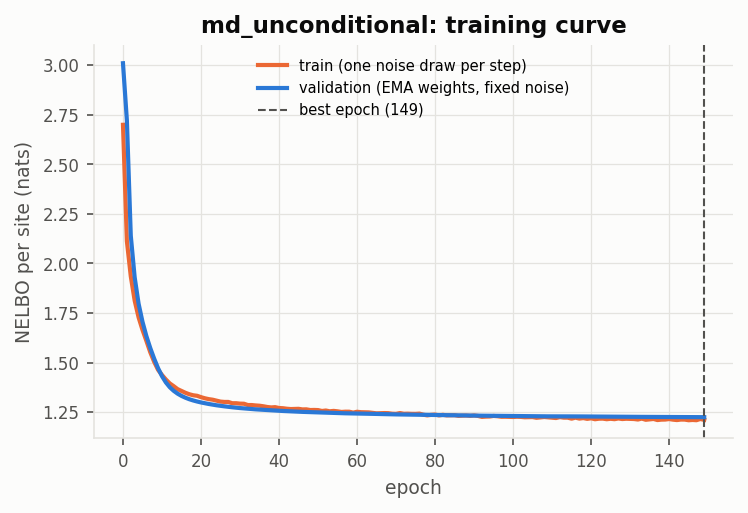
\includegraphics[width=0.55\linewidth]{models/md_unconditional/training_curve.png}
\caption{Training curve of the masked diffusion model (NELBO per site, nats). The two curves overlap; the last
100 epochs gain only 0.025.}
\end{figure}

\subsection{Checkpoints during training}\label{sec:md_checkpoints}
This first run kept its best model only in memory until the end. After it, checkpointing was added to
\texttt{train\_diffusion}, so that a run can be inspected at any time and survive an interruption:
\begin{center}\small
\begin{tabular}{p{0.3\linewidth}p{0.62\linewidth}}
\toprule
file (in \texttt{models/<run>/}) & content and when it is written\\
\midrule
\texttt{model.pt} & the best EMA model so far; rewritten every time the validation NELBO improves (and at the end)\\
\texttt{last.pt} & the complete training state after every epoch: network weights, EMA weights, AdamW moments, learning-rate
schedule, gradient-scaler state, the two random-number generators, history, best value, patience counter\\
\texttt{checkpoints/epoch\_XXX.pt} & a snapshot of the EMA model every \texttt{save\_every} epochs (default 10): the model at
different stages of training, e.g.\ to see how the samples improve\\
\bottomrule
\end{tabular}
\end{center}
\texttt{python scripts/s09\_train\_diffusion.py --config ... --resume} continues from \texttt{last.pt}. Because the optimiser,
schedule, scaler and random-number generators are restored, \textbf{a resumed run is identical to an uninterrupted one}.
\texttt{test\_16\_checkpointing} trains 4 epochs, resumes to 6, and checks that every loss value and every final weight equals
those of a 6-epoch run in one go. It also checks the files and that \texttt{model.pt} equals the returned best model.

\section{Results}\label{sec:md_results}
All comparisons use the held-out test set (1000 sequences per clade) and the same metrics as Part~II.

\subsection{Likelihood bound}
Test NELBO: \textbf{1.219 nats per site} (validation 1.225). This is an upper bound on $-\frac1L\log p_\theta(\bm x)$. The
true value for the data, the entropy per site of the 18-clade mixture, cannot be computed here: it needs the 18 partition
functions. For scale, an independent-site model scores 2.11.

\subsection{The probabilities themselves}
The one-site-masked output $p_\theta(x^i\mid\bm x_{-i})$ was compared, on all 18{,}000 test sequences and 60 sites, with the exact
conditional of the true model of the clade each sequence was drawn from:
\begin{center}\footnotesize
\begin{tabular}{lccc}
\toprule
model & uses the & pseudo-NLL & mean TV to the\\
 & clade label? & per site & true conditional\\
\midrule
true clade models & yes & 0.802 & 0\\
unconditioned Potts $H=128$ & no & 0.949 & 0.154\\
unconditioned Potts $H=256$ & no & 0.945 & 0.152\\
conditioned Potts $H=128$ (true tags) & \textbf{yes} & \textbf{0.872} & \textbf{0.100}\\
conditioned Potts $H=256$ (true tags) & yes & 0.887 & 0.113\\
\textbf{masked diffusion} & \textbf{no} & 0.883 & 0.102\\
\bottomrule
\end{tabular}
\end{center}
Without being told the clade, the diffusion model's conditionals are as close to the truth (TV 0.102) as those of the
best conditioned Potts model \emph{given} the true clade tag (0.100). The network infers the clade from the other 59
residues. Its pseudo-NLL is the second best (0.883 vs 0.872), far ahead of the unconditioned Potts models (0.95).

\begin{figure}[H]
\centering
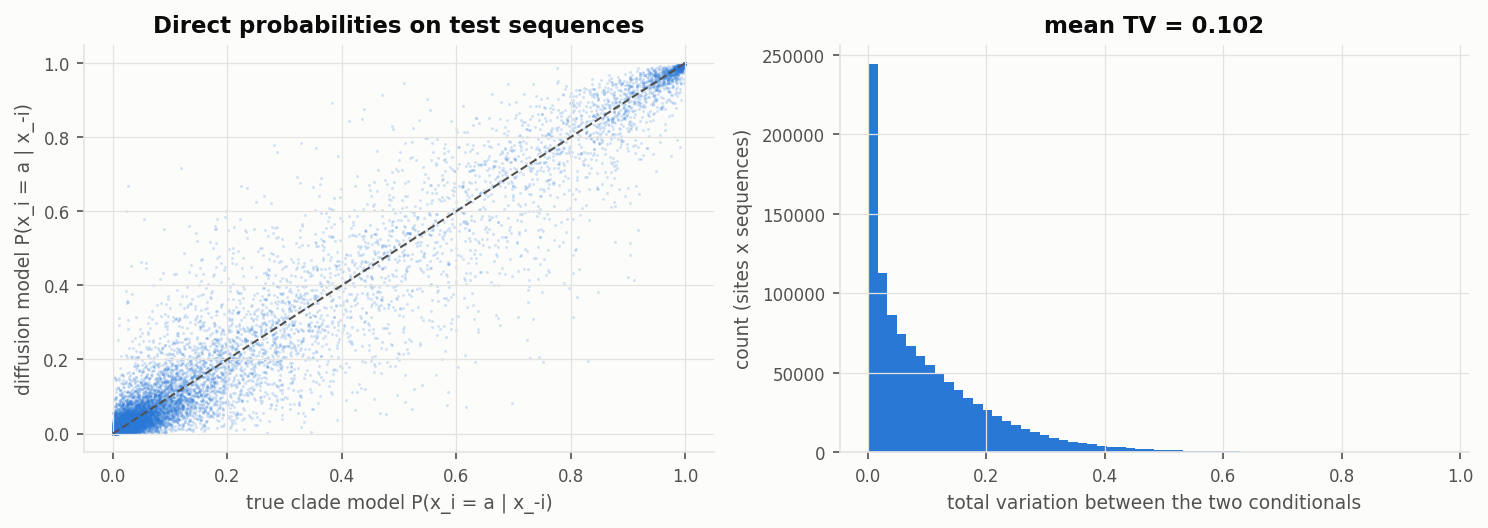
\includegraphics[width=0.85\linewidth]{models/md_unconditional/site_conditionals_vs_truth.png}
\caption{Left: $p_\theta(x^i=a\mid\bm x_{-i})$ vs the true clade conditional (60{,}000 random entries). Right: distribution of the TV
between the two distributions over all sites of all test sequences (median 0.07).}
\end{figure}

\paragraph{Does the network use $t$?} Theory says no (\S\ref{sec:md_optimal}). We fed the same partially masked test sequences
with different $t$ (\texttt{s12}). Changing $t$ from the matching value to anything in $[0.02,1]$ changes the predicted
distributions by a TV of only 0.004--0.03. Two \emph{different} sequences give predictions 0.34--0.56 apart. The network has
learned to (almost) ignore the time input; the small residual grows with the mask fraction.

\subsection{Samples: the sampler matters}
18{,}000 sequences each (as many as the test set):
\begin{center}\footnotesize
\begin{tabular}{lcccccc}
\toprule
sampler & $r_f$ & $r_C$ & slope $C$ & identity & F0/F1/F2 & $\bar d_{NN}$ to train\\
\midrule
$T=15$ steps & 0.999 & 0.987 & 0.81 & 0.197 & 32.3/36.7/30.7\% & 0.425\\
$T=60$ & 1.000 & 0.992 & 0.94 & 0.200 & 33.0/34.1/32.4\% & 0.401\\
$T=240$ & 1.000 & 0.992 & 0.98 & 0.201 & 33.0/32.5/33.7\% & 0.394\\
\textbf{continuous time} & \textbf{1.000} & \textbf{0.992} & \textbf{0.985} & 0.201 & \textbf{33.2/33.0/33.2\%} & 0.393\\
\midrule
oracle (true samples) & 1.000 & 0.994 & 0.99 & 0.197 & 33.1/32.7/33.3\% & 0.378\\
\bottomrule
\end{tabular}
\end{center}
As predicted by \S\ref{sec:md_sampler} and \texttt{test\_13}, few steps weaken the correlations: with $T=15$, about four sites are
revealed per step and drawn independently, and the slope of $C$ drops to 0.81. With $T=60$ it is 0.94, with $T=240$
0.98, and the exact continuous-time sampler reaches 0.985 for the cost of $T=60$. All results below use the
continuous-time sampler.

\begin{figure}[H]
\centering
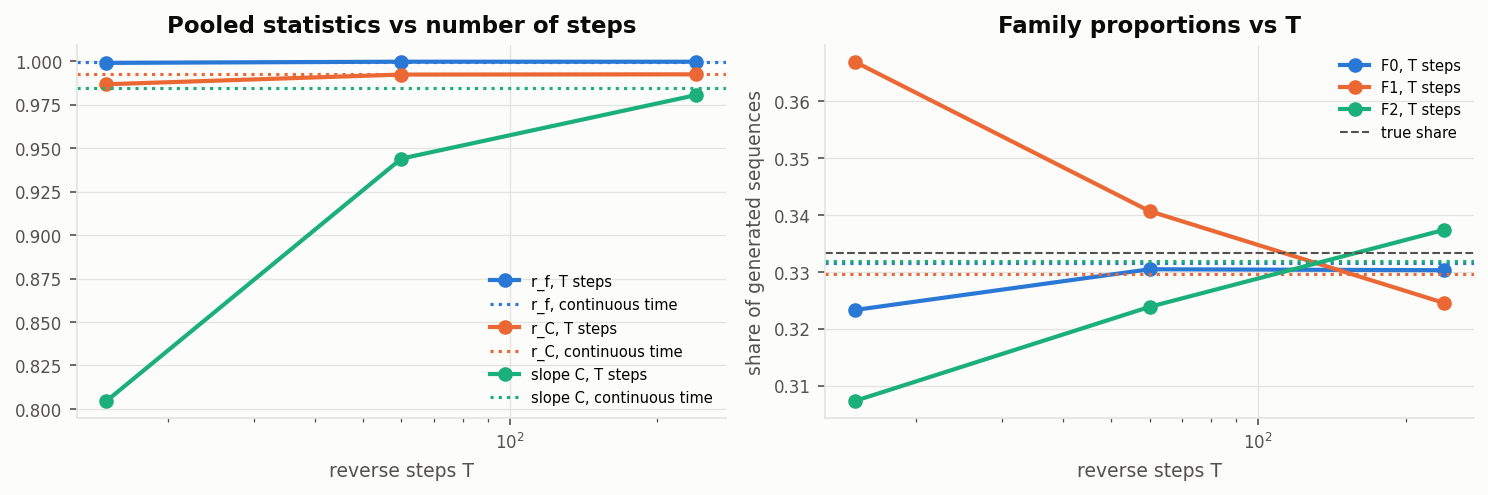
\includegraphics[width=0.9\linewidth]{models/md_unconditional/quality_vs_steps.png}
\caption{Pooled statistics and family proportions vs the number of reverse steps $T$ (dots) and for the continuous-time
sampler (dotted lines).}
\end{figure}

\subsection{Family and clade proportions: fixed}
\begin{center}\footnotesize
\begin{tabular}{lcc}
\toprule
 & family shares F0/F1/F2 & clade shares: TV to 1/18\\
\midrule
oracle & 33.3/33.3/33.3\% & 0.005\\
unconditioned Potts $H=128$ & 21.5/12.8/65.7\% & 0.324\\
unconditioned Potts $H=256$ & 10.7/13.6/75.7\% & 0.424\\
conditioned Potts $H=128$, 18 tags pooled & 33.3/33.3/33.3\% (by construction) & 0.013\\
\textbf{masked diffusion} & \textbf{33.4/33.4/33.2\%} & \textbf{0.011}\\
\bottomrule
\end{tabular}
\end{center}
(Clades are assigned with the pseudo-likelihood classifier of \texttt{s11}: each sequence goes to the true clade model under
which it has the highest pseudo-log-likelihood, which needs no partition function. On the labelled test sequences this
classifier is right for 91.5\% of the clades and 100\% of the families; \texttt{test\_10} checks it on a toy case.)

\textbf{The diffusion model generates the three families, and the 18 clades, in the right proportions}, with no labels,
where the unconditioned Potts models failed badly (\S\ref{sec:res_props}). This is the difference between the two losses.
Pseudo-likelihood never sees the normalisation, so it cannot balance the families. The NELBO bounds the full likelihood, so
a model that gives F2 too much weight pays for it in the loss.

\begin{figure}[H]
\centering
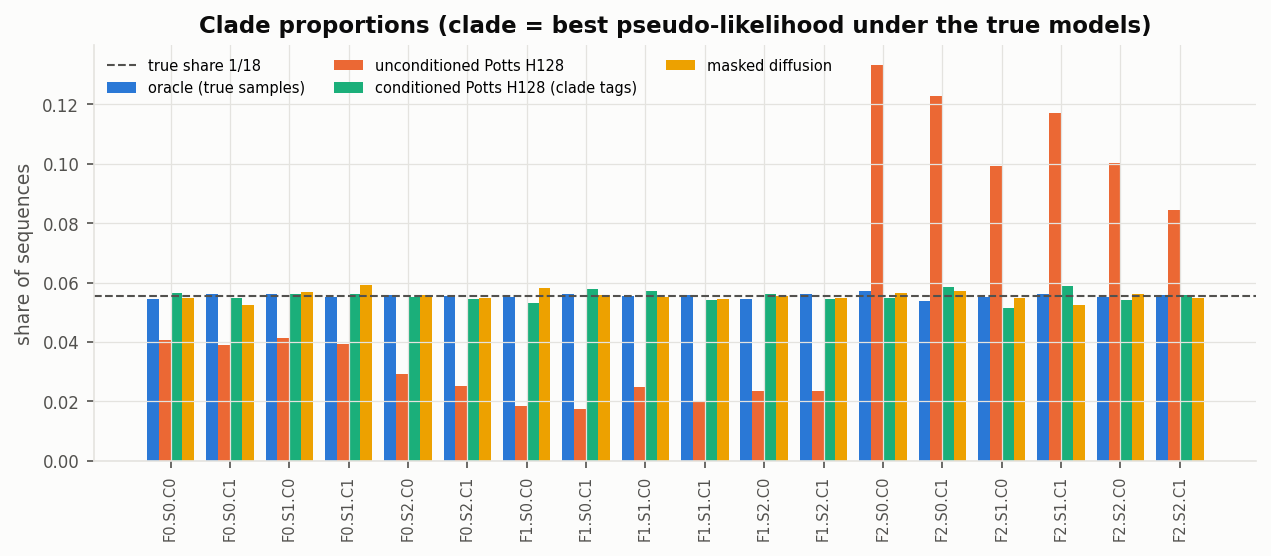
\includegraphics[width=\linewidth]{comparison/clade_proportions.png}
\caption{Share of generated sequences in each clade (assigned by pseudo-likelihood under the true models). Blue: true samples;
orange: unconditioned Potts (F2 clades over-represented); green: conditioned Potts with clade tags; yellow: masked diffusion.}
\end{figure}

\begin{figure}[H]
\centering
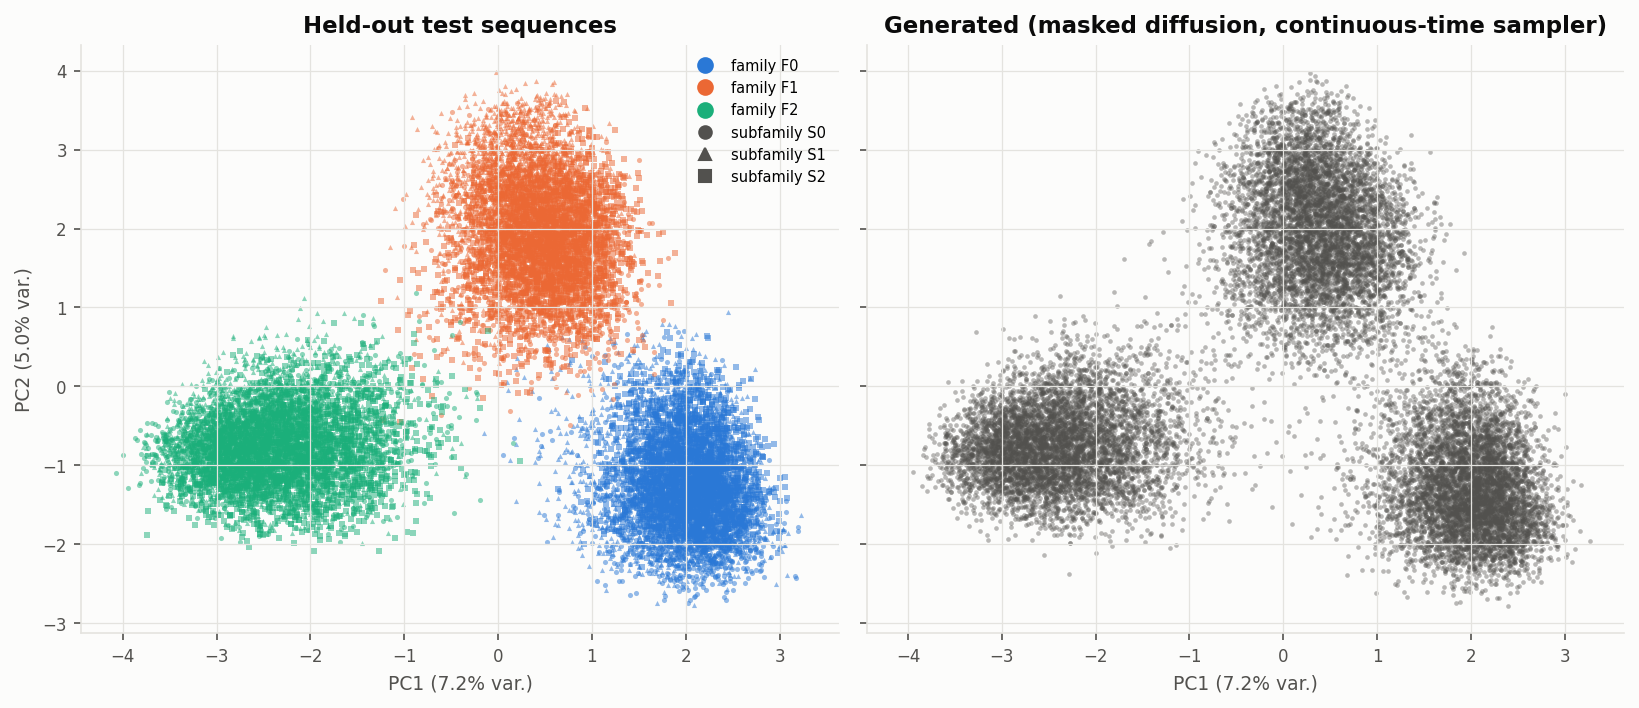
\includegraphics[width=0.85\linewidth]{models/md_unconditional/pca_generated_vs_test.png}
\caption{Test sequences (left) and diffusion samples (right) on the reference PCA: three equally populated families.}
\end{figure}

\subsection{Statistics and distances}
\begin{center}\footnotesize
\begin{tabular}{lcccc}
\toprule
 & unconditioned Potts $H=128$ & \textbf{masked diffusion} & oracle & (test)\\
\midrule
pooled $r_f$ / $r_C$ & 0.940 / 0.895 & \textbf{1.000 / 0.992} & 1.000 / 0.994 & \\
slope of $C$ & 0.70 & \textbf{0.985} & 0.99 & \\
per family: $r_C$ (mean) & 0.83 & \textbf{0.96} & -- & \\
per family: slope of $C$ (mean) & 0.66 & \textbf{0.89} & -- & \\
pairwise $\bar D_{GG}$ & 0.740 & \textbf{0.799} & 0.803 & 0.803\\
Fréchet distance (PCA, pooled) & 2.23 & \textbf{0.005} & 0.001 & \\
mean $d_{NN}$ to train & 0.398 & 0.393 & 0.378 & 0.378\\
copies of training sequences & 0 & 0 & 0 & \\
\bottomrule
\end{tabular}
\end{center}
The pooled statistics are practically those of true samples. Inside each family the correlations are reproduced at
$r_C=0.96$, with a slope of 0.89: slightly too weak, the same direction of error as all previous models but much
smaller. The generated sequences are as diverse as real ones (0.799 vs 0.803), and not copies. They are slightly
\emph{farther} from the training set than real held-out sequences (0.393 vs 0.378, i.e.\ about one site out of 60). This is a
small excess of randomness, consistent with the slightly weak correlations.

\begin{figure}[H]
\centering
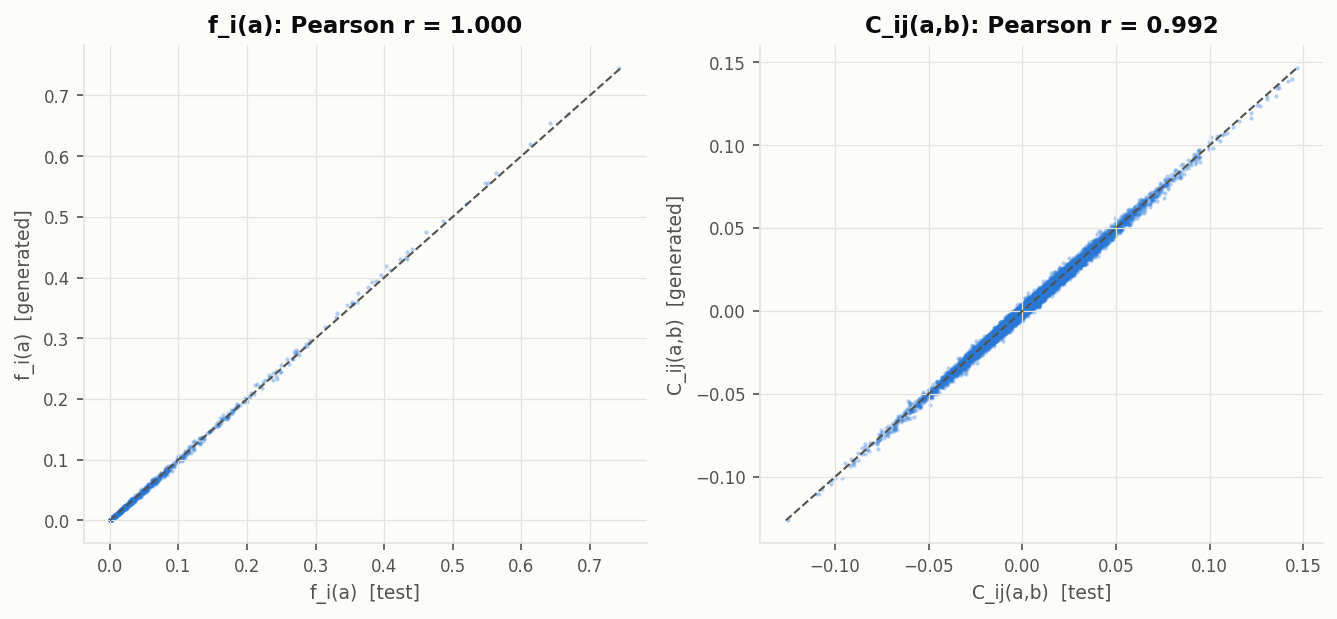
\includegraphics[width=0.49\linewidth]{models/md_unconditional/freq_corr_generated_vs_test.png}\hfill
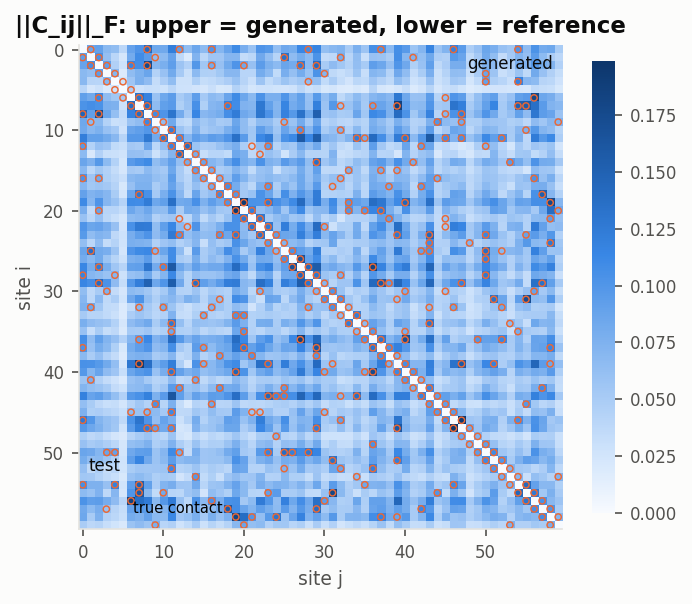
\includegraphics[width=0.4\linewidth]{models/md_unconditional/correlation_strength_test_vs_generated.png}
\caption{Left: site frequencies and connected correlations, diffusion samples vs test. Right: correlation strength map
(lower: test, upper: generated).}
\end{figure}

\begin{figure}[H]
\centering
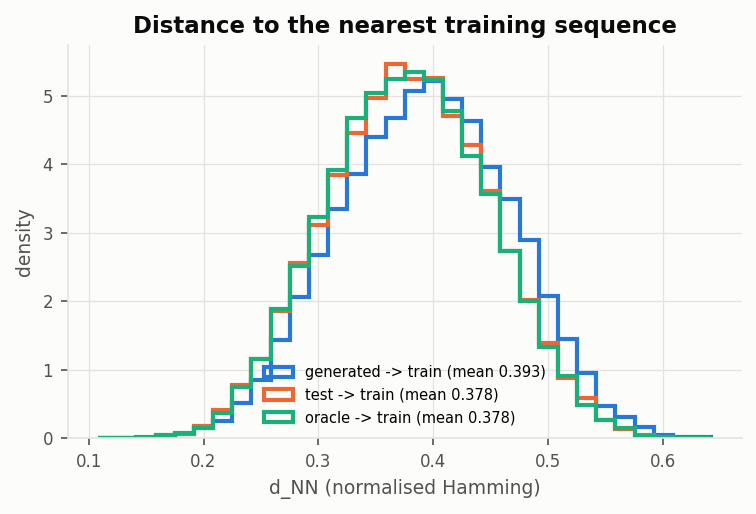
\includegraphics[width=0.49\linewidth]{models/md_unconditional/dist_nn_to_train.png}\hfill
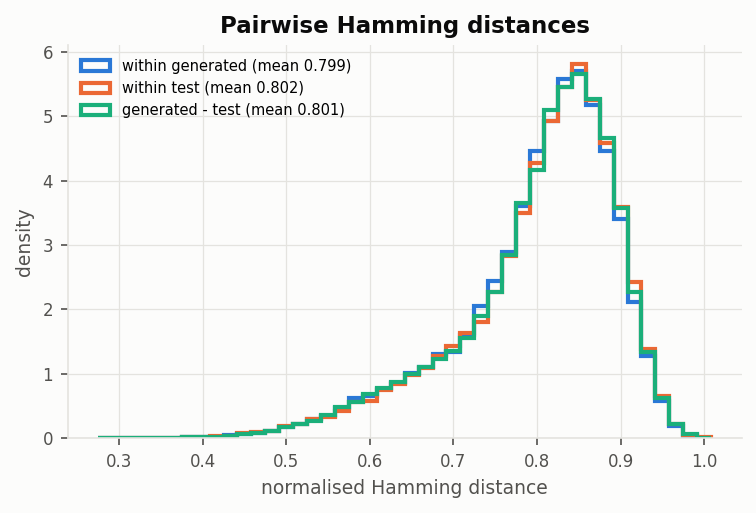
\includegraphics[width=0.49\linewidth]{models/md_unconditional/dist_pairwise.png}
\caption{Distances: nearest training sequence (left) and pairwise Hamming distances (right) for diffusion samples, test and oracle.}
\end{figure}

\subsection{All models at the clade level}
The unconditioned diffusion model can also be judged clade by clade: the generated sequences assigned to clade $c$ are
compared with the test sequences of clade $c$.
\begin{center}\footnotesize
\begin{tabular}{lcccc}
\toprule
 & uses labels & per-clade $r_C$ & per-clade Fréchet & clade shares, TV to 1/18\\
\midrule
oracle & -- & 0.828 & 0.032 & 0.005\\
unconditioned Potts $H=128$ & no & 0.562 & 1.716 & 0.324\\
unconditioned Potts $H=256$ & no & 0.555 & 1.448 & 0.424\\
conditioned Potts $H=128$ & \textbf{yes (tags)} & 0.751 & 0.332 & 0.013\\
\textbf{masked diffusion} & \textbf{no} & \textbf{0.764} & \textbf{0.136} & \textbf{0.011}\\
\bottomrule
\end{tabular}
\end{center}
\begin{figure}[H]
\centering
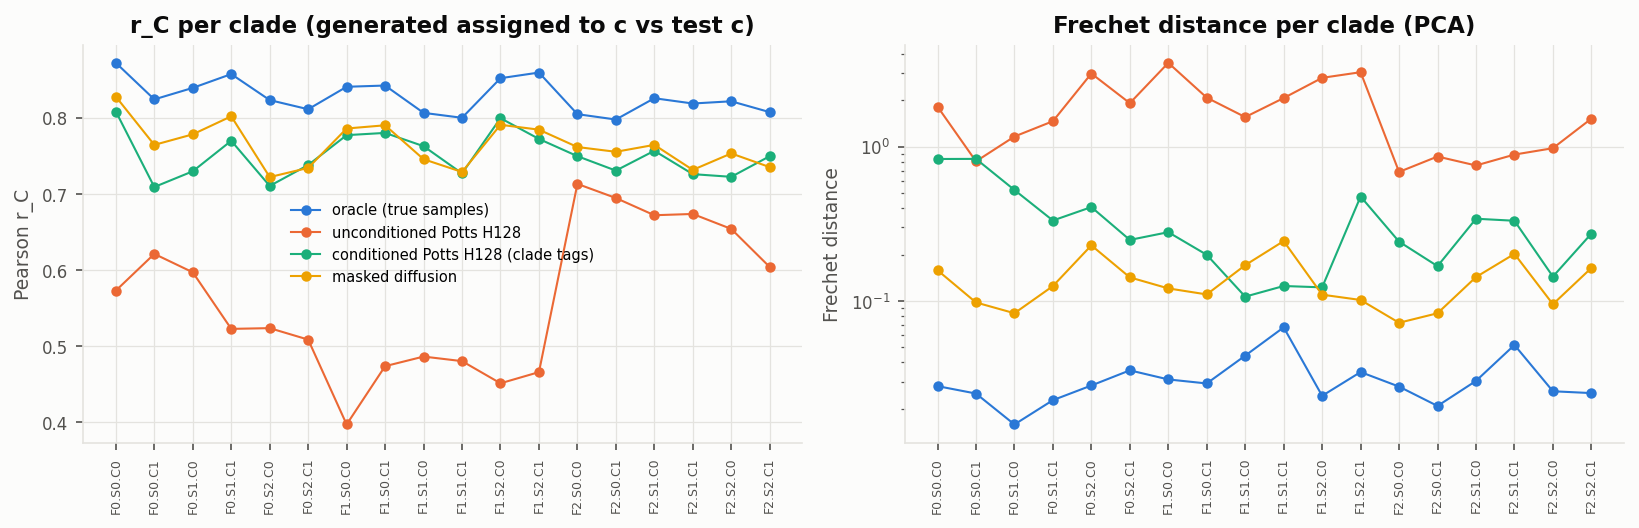
\includegraphics[width=\linewidth]{comparison/per_clade_quality.png}
\caption{Per-clade $r_C$ and Fréchet distance (log scale) of the generated sequences assigned to each clade, for all models.}
\end{figure}

\begin{keybox}{Masked diffusion: summary}
\begin{itemize}[nosep]
\item[+] \textbf{Right global weights}: families 33/33/33\%, clades within 0.011 of uniform, without labels. Training on a
      likelihood bound fixes the main failure of the pseudo-likelihood models.
\item[+] \textbf{Best generator so far}: pooled $r_C=0.992$ (oracle 0.994), Fréchet 0.005 (oracle 0.001); per clade it matches or beats
      the conditioned Potts model that is \emph{given} the clade tag ($r_C$ 0.764 vs 0.751, Fréchet 0.14 vs 0.33).
\item[+] \textbf{Correct probabilities}: its conditionals are as close to the true clade conditionals (TV 0.10) as those of the
      tag-conditioned Potts model; it infers the clade from the sequence.
\item[+] No memorisation; diversity equal to real sequences.
\item[--] Correlations inside a family are still $\approx10\%$ too weak (slope 0.89), and the samples are about one site more
      ``random'' than real sequences. Training had not fully converged (best epoch $=$ last epoch).
\item[--] It gives no interpretable $J$; the price of not assuming a Potts form. It is also 2--9$\times$ larger (4.8\,M parameters vs 0.5--2.1\,M)
      and 10--100$\times$ more expensive to train than the factored-attention models (4\,h vs 2--23\,min).
\item[!] The sampler matters: few reverse steps destroy correlations; use the exact continuous-time sampler.
\end{itemize}
\end{keybox}


% ==========================================================================================
% PART IV : dynamical regimes (speciation and collapse) of the masked diffusion model
% ==========================================================================================
\part{Dynamical regimes: speciation and collapse}

\section{The question}\label{sec:dr_question}
A diffusion model generates a sequence gradually. In our masked model, it starts from a fully hidden sequence
($t=1$) and reveals residues one after the other until $t=0$. Two questions can be asked about this process.
\begin{enumerate}[nosep]
\item \textbf{When does a trajectory decide which family, subfamily, or clade it will belong to?} At $t=1$ nothing is
decided. At $t=0$ the sequence is complete, so its class is fixed. Somewhere in between, the trajectory
\emph{commits}. That moment is the \textbf{speciation time} $t_S$. With a tree of classes we expect one speciation time
per level: the family is chosen first, then the subfamily, then the clade.
\item \textbf{When would a trajectory decide which \emph{training sequence} it will reproduce?} The loss we train on
has an exact minimiser, the \emph{empirical} denoiser. It only knows the $n$ training sequences, so it can only
regenerate them (memorisation). Along its trajectories there is a moment after which the final training sequence is
fixed. That is the \textbf{collapse time} $t_C$ (the ``condensation'' of the trajectory onto one data point).
\end{enumerate}
Both notions come from Biroli, Bonnaire, de Bortoli and Mézard, \emph{Dynamical regimes of diffusion models},
Nature Communications 15, 9957 (2024). They studied diffusion with \emph{Gaussian} noise in high dimension $d$ and
found three regimes in the backward (generation) process:
\begin{center}\small
\begin{tabular}{llp{9cm}}
\toprule
regime & backward time & what the trajectory knows\\
\midrule
I & $t>t_S$ & nothing: it could still end in any class\\
II & $t_C<t<t_S$ & its class, but not a specific data point (the \emph{generalisation} regime)\\
III & $t<t_C$ & the exact training point it will reproduce (only for the empirical score: memorisation)\\
\bottomrule
\end{tabular}
\end{center}
They obtained $t_S$ from the spectrum of the data covariance and $t_C$ from an entropy argument borrowed from the
statistical physics of disordered systems (the Random Energy Model).

This part does three things. First, it re-derives both results for Gaussian noise (\S\ref{sec:dr_gauss}), because
the derivations show what to transpose. Second, it transposes them to masking (\S\ref{sec:dr_mask_spec},
\S\ref{sec:dr_mask_coll}). Masking turns out to make several statements \emph{exact} rather than asymptotic. Third,
it measures both times on our trained model and on the data (\S\ref{sec:dr_results}).

%==========================================================================================
\section{The Gaussian case (the paper's setting)}\label{sec:dr_gauss}
%==========================================================================================
\subsection{Forward process}
The data $\bm x_0\in\mathbb R^d$ are noised by the Ornstein--Uhlenbeck process
$d\bm x=-\bm x\,dt+\sqrt2\,d\bm B_t$, whose solution is
\begin{equation}\label{eq:ou}
\bm x_t=e^{-t}\bm x_0+\sqrt{\Delta_t}\,\bm\xi,\qquad \Delta_t=1-e^{-2t},\qquad \bm\xi\sim\mathcal N(0,I_d).
\end{equation}
The signal shrinks as $e^{-t}$ and the noise variance grows to 1. Generation runs this backwards, from pure noise at
large $t$ to $t=0$, using the score $\nabla\log P_t$ (in practice, a network trained to approximate it).

\subsection{Speciation: two Gaussian classes}\label{sec:dr_gauss_spec}
Take two equally likely classes, $\bm x_0=\pm\bm m+\sigma\bm z$ with $\bm z\sim\mathcal N(0,I_d)$. By
\eqref{eq:ou}, given the class, $\bm x_t$ is Gaussian with mean $\pm e^{-t}\bm m$ and variance
$\Gamma_t=\sigma^2e^{-2t}+\Delta_t$ in every direction. So $P_t$ is a mixture of two Gaussians.

\paragraph{The class posterior.} By Bayes' rule, the log-odds of class $+$ against class $-$ given $\bm x_t$ is the
difference of the two Gaussian exponents:
\[
\Lambda(\bm x_t)=\log\frac{P(+\mid\bm x_t)}{P(-\mid\bm x_t)}
=\frac{\|\bm x_t+e^{-t}\bm m\|^2-\|\bm x_t-e^{-t}\bm m\|^2}{2\Gamma_t}=\frac{2e^{-t}\,\bm m\cdot\bm x_t}{\Gamma_t}.
\]
(The $\|\bm x_t\|^2$ and $\|\bm m\|^2$ terms cancel.) Now let $\bm x_t$ come from class $+$. Then
$\bm m\cdot\bm x_t=e^{-t}\|\bm m\|^2+\sqrt{\Gamma_t}\,\|\bm m\|\,g$ with $g\sim\mathcal N(0,1)$, since the projection of
isotropic noise of variance $\Gamma_t$ on the direction of $\bm m$ has variance $\Gamma_t\|\bm m\|^2$. Therefore
\begin{equation}\label{eq:llr_gauss}
\Lambda=\mu_t+\sqrt{2\mu_t}\,g,\qquad \mu_t=\frac{2\|\bm m\|^2e^{-2t}}{\Gamma_t}.
\end{equation}
The log-odds is Gaussian with mean $\mu_t$ and variance $4\|\bm m\|^2e^{-2t}/\Gamma_t=2\mu_t$. This mean/variance
relation is not an accident. A log-likelihood ratio must satisfy $\E_-[e^{\Lambda}]=1$ (the likelihood ratio averages
to 1 under the other class), and for a Gaussian $\Lambda$ this forces variance $=2\times$mean. We call $\mu_t$ the
\textbf{class signal-to-noise ratio}.

\paragraph{The cloning experiment.} The paper measures commitment like this: stop a backward trajectory at time $t$,
make two copies (``clones''), and continue both independently to $t=0$. Given $\bm x_t$, each clone ends in class
$+$ with probability $p=P(+\mid\bm x_t)$. So the two clones end in the same class with probability $p^2+(1-p)^2$.
Averaging over $\bm x_t$:
\begin{equation}\label{eq:phi_def}
\phi(t)=\E_{\bm x_t}\Big[\sum_cP(c\mid\bm x_t)^2\Big].
\end{equation}
$\phi$ goes from $\sum_c\pi_c^2=1/2$ (nothing decided) to 1 (decided). Normalise it to run from 0 to 1:
$\psi=(\phi-\phi_0)/(1-\phi_0)$. For two classes, $p=1/(1+e^{-\Lambda})$ gives
$p^2+(1-p)^2=\tfrac12\big(1+(2p-1)^2\big)=\tfrac12\big(1+\tanh^2(\Lambda/2)\big)$. Hence
\begin{equation}\label{eq:psi_universal}
\boxed{\psi=\E\big[\tanh^2(\Lambda/2)\big]=:\Psi(\mu),\qquad \Lambda\sim\mathcal N(\mu,2\mu).}
\end{equation}
The commitment is a \emph{universal} function of the single number $\mu$. It is 0 at $\mu=0$, tends to 1 as
$\mu\to\infty$, and crosses $1/2$ at $\mu^\star=1.70$ (computed numerically).

\paragraph{The speciation time.} Define $t_S$ by $\psi(t_S)=1/2$, i.e.\ $\mu_{t_S}=\mu^\star$. Speciation happens when
the noise is already large, so $\Gamma_t\approx1$, and
\begin{equation}\label{eq:ts_gauss}
2\|\bm m\|^2e^{-2t_S}=\mu^\star\ \Longrightarrow\ t_S=\tfrac12\log\|\bm m\|^2+\tfrac12\log(2/\mu^\star)\approx\tfrac12\log\Lambda_{\max}.
\end{equation}
The covariance of the data is $\bm m\bm m^\top+\sigma^2I$, whose largest eigenvalue is
$\Lambda_{\max}=\|\bm m\|^2+\sigma^2\approx\|\bm m\|^2$. In high dimension $\Lambda_{\max}$ grows with $d$, and the
$O(1)$ constant is negligible. That gives the paper's formula $t_S=\tfrac12\log\Lambda_{\max}$.

\paragraph{The same time, seen as a symmetry breaking.} The paper derives $t_S$ from the shape of the potential
$U_t=-\log P_t$, which drives the backward dynamics. Along the direction of $\bm m$ at the midpoint $\bm x=0$,
differentiating the two-Gaussian mixture twice gives a curvature
$\partial^2\log P_t=-1/\Gamma_t+e^{-2t}\|\bm m\|^2/\Gamma_t^2$. For large $t$ it is negative: a single well, and
the trajectory is not attracted to either class. It changes sign when $e^{-2t}\|\bm m\|^2=\Gamma_t\approx1$, the same
$t_S$ up to the $O(1)$ constant. Below $t_S$ the potential has two wells and each trajectory falls into one: the
symmetry between classes is broken. \texttt{test\_17} simulates this two-Gaussian system ($d=50$,
$\|\bm m\|^2=400$). It checks that the measured commitment follows $\Psi(\mu_t)$ at every $t$ and crosses 1/2 at
$\tfrac12\log(2\|\bm m\|^2/\mu^\star)$ (Fig.~\ref{fig:dr_tests}, left).

\subsection{Collapse: the empirical score and the Random Energy Model}\label{sec:dr_gauss_coll}
Now suppose the model has learned the score of the \emph{empirical} distribution of $n$ training points
$\bm a_1,\dots,\bm a_n$ (the exact minimiser of the denoising loss on the training set). The noised empirical
distribution is a mixture of $n$ small Gaussians:
\[
P^e_t(\bm x)=\frac1n\sum_{\mu=1}^n\mathcal N\big(\bm x;\,e^{-t}\bm a_\mu,\,\Delta_tI\big).
\]
The backward process with this score reproduces $P^e_t$ at every time. At $t=0$ it therefore returns a training
point. A trajectory that ends at $\bm a_1$ is, at time $t$, $\bm x_t=e^{-t}\bm a_1+\sqrt{\Delta_t}\bm\xi$. How strongly
does it already ``belong'' to $\bm a_1$? Compare the Gaussian weight of $\bm a_1$ with the total weight of all the
others:
\[
w_1=\mathcal N(\bm x_t;e^{-t}\bm a_1,\Delta_t)\approx(2\pi e\Delta_t)^{-d/2},
\qquad \sum_{\mu\ge2}w_\mu\approx(n-1)\,\E_{\bm a}\big[\mathcal N(\bm x_t;e^{-t}\bm a,\Delta_t)\big]=(n-1)P_t(\bm x_t).
\]
The first uses $\|\bm\xi\|^2\approx d$. The second is the law of large numbers: the other training points are
independent draws from the true $P_0$, and averaging the Gaussian kernel over $P_0$ gives the true noised density
$P_t$. With $-\frac1d\log P_t(\bm x_t)\approx s(t)$, the entropy per dimension of $P_t$:
\begin{equation}\label{eq:collapse_gauss}
\frac{\sum_{\mu\ge2}w_\mu}{w_1}\approx n\,e^{-d\,f(t)},\qquad f(t)=s(t)-\tfrac12\log(2\pi e\Delta_t).
\end{equation}
$f(t)$ is the \textbf{excess entropy}: the entropy of $P_t$ minus the entropy of the noise alone. It measures how many
distinguishable ``noise balls'' the data occupy. While $n e^{-d f(t)}\gg1$, the other points dominate: the trajectory
is surrounded by many training points and has not chosen. When $n e^{-d f(t)}\ll1$, $\bm a_1$ dominates and the
trajectory has collapsed. The collapse time solves
\begin{equation}\label{eq:tc_gauss}
\boxed{f(t_C)=\frac{\log n}{d}.}
\end{equation}
The law-of-large-numbers step fails exactly at $t_C$. Below it, the sum over $\mu$ is dominated by a single term, as
the partition function of the Random Energy Model is dominated by its lowest energy levels below the glass
(``condensation'') transition. This is why the paper borrows REM methods, and why the typical (``quenched'') and the
average (``annealed'') values of the sum differ.

\paragraph{The picture.} Speciation depends on the class structure (the top eigenvalue), not on $n$. Collapse
depends on $n$: more data pushes $t_C$ to smaller $t$, and for $\log n\propto d$ the two are well separated. A
network trained on the same data \emph{generalises} if it does not reproduce the empirical score below $t_C$.

%==========================================================================================
\section{From Gaussian noise to masking}\label{sec:dr_mask}
%==========================================================================================
\subsection{Time, revealed sites, and what the noise does}
In our model (Part~III) the noise is masking. At time $t$ every site is hidden independently with probability $t$,
so the number of \textbf{revealed sites} is $k\sim\mathrm{Binomial}(L,1-t)$, with mean $L(1-t)$. Given $k$, the set
$U$ of revealed sites is a uniformly random $k$-subset, \emph{independent of the sequence}. Everything below is
therefore computed at fixed $k$ and converted to $t$ at the end:
\begin{equation}\label{eq:k_to_t}
\langle f\rangle(t)=\sum_{k=0}^L\binom Lk(1-t)^kt^{L-k}\,f_k .
\end{equation}
Because the mask is independent of the data, the posterior over the clean sequence is just the data distribution
conditioned on the revealed residues:
\begin{equation}\label{eq:mask_posterior}
P(\bm x_0\mid\bm x_t)=P(\bm x_0\mid \bm x_U)\propto P(\bm x_0)\,\one[\bm x_{0,U}=\bm x_U].
\end{equation}
Two differences with Gaussian noise matter.
\begin{itemize}[nosep]
\item A revealed residue is \emph{exact}, and a hidden one carries \emph{no} information. There is no partial
information per site.
\item The reverse direction is ``$k$ grows'': $k=0$ at $t=1$ (start of generation) and $k=L$ at $t=0$. A
\emph{large} speciation time $t_S$ means the class is decided \emph{early}, after few revealed sites.
\end{itemize}

\subsection{Speciation for masking}\label{sec:dr_mask_spec}
\paragraph{Cloning, exactly.} Let $y(\bm x)$ be any deterministic label of complete sequences, for instance the clade
assigned by a classifier. From a partially revealed $\bm x_t$, complete it $C$ times independently with the denoiser
(``clones''). With the exact denoiser, each completion is an independent draw from $P(\bm x_0\mid\bm x_U)$, so
\begin{prop}[clone agreement]\label{prop:clone}
With the exact denoiser, (i) two clones get the same label with probability
$\phi_k=\E\big[\sum_yP(y\mid\bm x_U)^2\big]$; (ii) a clone gets the \emph{same label as the original sequence} with the
same probability $\phi_k$.
\end{prop}
\emph{Proof.} (i) Given $\bm x_U$ the clones are independent with label distribution $P(y\mid\bm x_U)$, so they agree
with probability $\sum_yP(y\mid\bm x_U)^2$; then average. (ii) The original $\bm x_0$ is itself a draw from
$P(\bm x_0\mid\bm x_U)$, independent of the clones given $\bm x_U$, so the same computation applies. $\square$

Part (ii) gives a consistency check on a \emph{trained} network. If its clones agree with each other more (or less)
than with the original, its conditional distributions are wrong.

\paragraph{The network's own trajectories.} The exact continuous-time sampler (Part~III) reveals sites in a uniformly
random order at independent random times, both drawn independently of the residues. So at any time $t$ of a
generated trajectory, $\bm x_t$ is the final sample with a random, sequence-independent set of sites hidden.
\emph{Masking the network's samples therefore gives exactly its trajectories at time $t$.} We use two starting
ensembles: (A) masked \textbf{held-out true} sequences, which probe the network on the true $\bm x_t$; and (B) masked
\textbf{network samples}, which are its own trajectories.

\paragraph{Theory: the class log-odds for masking.} Let each class $c$ be summarised by its site frequencies
$f_{c,i}(a)$ (the \emph{profile} approximation, which ignores couplings). Given the revealed residues, Bayes' rule
gives
\begin{equation}\label{eq:profile_post}
\log P(c\mid\bm x_U)=\log\pi_c+\sum_{i\in U}\log f_{c,i}(x_i)-\text{normaliser}.
\end{equation}
Between two classes $c,c'$ the log-odds is a sum over revealed sites,
$\Lambda=\sum_{i\in U}\log\frac{f_{c,i}(x_i)}{f_{c',i}(x_i)}$. For $\bm x$ from $c$, each site contributes on average
$\mathrm{KL}(f_{c,i}\|f_{c',i})$, and each site is revealed with probability $k/L$. Hence
\begin{equation}\label{eq:mu_mask}
\E\Lambda=\mu_k=\frac kL\,D,\qquad D=\sum_{i=1}^L\mathrm{KL}(f_{c,i}\,\|\,f_{c',i}).
\end{equation}
\emph{Variance.} Write $f_{c',i}=f_{c,i}(1+\varepsilon_i)$ with small $\varepsilon_i$. The per-site log-ratio
$r_i=-\log(1+\varepsilon_i)$ has mean $\mathrm{KL}_i\approx\frac12\E\varepsilon_i^2$ and variance
$\approx\E\varepsilon_i^2=2\,\mathrm{KL}_i$. Summing independent sites gives $\mathrm{Var}\,\Lambda\approx2\mu_k$: the
same ``variance $=2\times$mean'' law as \eqref{eq:llr_gauss}. When many weakly informative sites are revealed,
$\Lambda$ is approximately Gaussian, and the commitment follows the \emph{same universal curve} $\Psi(\mu)$ of
\eqref{eq:psi_universal}, with the time dependence
\begin{equation}\label{eq:snr_compare}
\text{Gaussian noise: }\mu_t\approx2\Lambda_{\max}e^{-2t},\qquad\qquad\text{masking: }\mu_t=(1-t)\,D.
\end{equation}
Setting $\mu=\mu^\star$:
\begin{equation}\label{eq:ts_mask}
\boxed{k_S=\frac{L\,\mu^\star}{D},\qquad t_S=1-\frac{\mu^\star}{D}.}
\end{equation}
The role of the top covariance eigenvalue is played by $D$, the total information that a fully revealed sequence
carries about its class relative to a sibling class. For our tree, the siblings of each level are the classes that
share the same parent. The hierarchy then predicts a \textbf{cascade of speciations}:
$D_{\rm family}>D_{\rm subfamily}>D_{\rm clade}$, so families are decided first, then subfamilies, then clades. With
the measured profiles (\S\ref{sec:dr_results}) $D=64,\,23,\,10$ nats, so
$k_S\approx1.6,\,4.4,\,9.8$ revealed sites.

Two caveats. (1) With few revealed sites, $\Lambda$ is a sum of a few terms and is not Gaussian. We therefore also
compute the \emph{profile-Bayes} commitment exactly, by Monte Carlo over true sequences and random masks with
\eqref{eq:profile_post}. (2) Couplings carry extra class information (in our tree, parent-to-child perturbations
also change $J$), and pairs of revealed residues can reveal it. The true commitment can therefore rise earlier than
the profile prediction.

\paragraph{A data-only estimate.} Before collapse, many training sequences agree exactly with $\bm x_U$. Their class
labels give a model-free estimate of $P(c\mid\bm x_U)$: the fraction of matching training sequences in class $c$. We
use it only when at least 20 sequences match. It is exact as $n\to\infty$ and, by construction, is available only
in regime I and early regime II. This is where the two times meet.

\subsection{Collapse for masking}\label{sec:dr_mask_coll}
\paragraph{The empirical denoiser.} Put the uniform distribution on the $n$ training sequences into
\eqref{eq:mask_posterior}. The posterior is uniform over the $N$ training sequences that agree with $\bm x_t$ on every
revealed site:
\begin{equation}\label{eq:emp_post}
P^e(\bm x_0=\bm a_\mu\mid\bm x_t)=\frac{\one[\bm a_{\mu,U}=\bm x_U]}{N(\bm x_t)},\qquad
N(\bm x_t)=\sum_{\mu=1}^n\one[\bm a_{\mu,U}=\bm x_U].
\end{equation}
Applying Proposition~\ref{prop:clone} with the label ``which training sequence'': \textbf{two clones end at the same
training sequence with probability $\E[1/N]$.} This is the collapse analogue of $\phi$. It is $1/n$ at $k=0$ and 1
once $N=1$.

\paragraph{How many training sequences match?} Follow a trajectory of the empirical denoiser that ends at training
sequence $\bm a_1$ (it is planted on $\bm a_1$). The planted sequence always matches. Each of the $n-1$ others is an
independent draw from the true distribution and matches with probability $P(\bm a_{1,U})$, the true probability of the
revealed residues. So, exactly,
\[
N=1+\mathrm{Binomial}\big(n-1,\ P(\bm a_{1,U})\big)\approx1+\mathrm{Poisson}(\lambda),\qquad \lambda=(n-1)\,P(\bm a_{1,U}).
\]
For $M\sim\mathrm{Poisson}(\lambda)$:
$\E\big[\tfrac1{1+M}\big]=\sum_m\frac{e^{-\lambda}\lambda^m}{(m+1)!}=\frac{e^{-\lambda}}\lambda\sum_{m\ge1}\frac{\lambda^m}{m!}
=\frac{1-e^{-\lambda}}{\lambda}$. Therefore
\begin{equation}\label{eq:collapse_mask}
\boxed{\E[1/N]=\E_{\bm a,U}\Big[\frac{1-e^{-\lambda}}{\lambda}\Big],\qquad \lambda=(n-1)P(\bm a_U).}
\end{equation}
This is the \textbf{quenched} prediction: the average is taken over the actual fluctuating $\lambda$. It crosses $1/2$
at $\lambda=1.59$. For typical $\bm a$, $-\log P(\bm a_U)\approx H(k)$, the entropy of $k$ revealed residues
(asymptotic equipartition), so collapse happens when
\begin{equation}\label{eq:tc_mask}
\boxed{H(k_C)=\log n.}
\end{equation}
This is \eqref{eq:tc_gauss} for masking. The ``excess entropy'' is simply $H(k)$, the entropy of the revealed
residues. A revealed residue carries no noise, so the ``noise ball'' around a data point contains exactly one
sequence (entropy 0), and nothing needs to be subtracted.

\paragraph{The annealed prediction, and why it is wrong.} Averaging $\lambda$ first replaces $P(\bm a_U)$ by its mean
$\E_{\bm a}P(\bm a_U)=\sum_{\bm x_U}P(\bm x_U)^2$. This is the probability that two independent sequences agree on the
$k$ revealed sites, and it can be read off pairwise Hamming distances. A pair at distance $D_{ab}$ agrees on a random
$k$-subset iff none of its $D_{ab}$ mismatches is revealed:
\begin{equation}\label{eq:collision}
\E_{\bm a}P(\bm a_U)=\E_{\text{pairs}}\Big[\binom{L-D_{ab}}{k}\Big/\binom Lk\Big]=e^{-H_2(k)},
\end{equation}
where $H_2$ is the Rényi-2 (collision) entropy. Since $H_2\le H$ (Jensen), the annealed average counts \emph{more}
matches than a typical trajectory sees. It is dominated by rare close pairs (same clade, small $D_{ab}$), exactly as
the annealed REM partition function is dominated by rare low energies. So it predicts a \emph{later} collapse (larger
$k_C$). The quenched formula \eqref{eq:collapse_mask} is the correct one; we show both.

\paragraph{Getting $H(k)$ from the network.} Let $i_1,i_2,\dots$ be the reveal order. By the chain rule,
\[
\log P(\bm x_{U_k})=\sum_{j=0}^{k-1}\log P\big(x_{i_{j+1}}\mid\bm x_{U_j}\big).
\]
The trained denoiser provides every factor,
so one pass of $L$ network calls gives $\log P_\theta(\bm x_{U_k})$ for all $k$. Averaged over sequences and orders,
$-\log P_\theta(\bm x_{U_L})$ is the NELBO of Part~III. Because the network's conditionals are close to the truth
(TV 0.10, Part~III), $P_\theta$ is a good stand-in for $P$ in \eqref{eq:collapse_mask}. It slightly overestimates
entropies, since a cross-entropy is at least the entropy.

\paragraph{Collapse versus $n$: the phase diagram.} $\log n$ enters only through \eqref{eq:collapse_mask}. So from
the same $P_\theta(\bm x_U)$ we can predict $k_C(n)$ for any $n$, and measure it directly on training subsets of size
$n$. Speciation at level $\ell$ happens before collapse (regimes cleanly separated) only if
\[
H(k_S^\ell)<\log n\iff n>n^\star_\ell=e^{H(k_S^\ell)}.
\]
For a small training set, the empirical denoiser picks a training sequence before it has even decided the clade, so
the clade is inherited from the memorised sequence.

\paragraph{Memorisation of the trained network.} The empirical denoiser is the \emph{exact minimiser} of the training
loss. Its NELBO on training data is $\log n/L$ nats per site, and it is infinite on new data. A network that reached it
would reproduce training sequences: along its trajectories, $\bm x_t$ would always match at least one training
sequence ($N\ge1$), as for planted trajectories. A generalising network produces trajectories that stop matching
the training set, like held-out true sequences do. We compare $P(N\ge1)$ along three kinds of trajectories:
planted on training sequences (always 1), held-out sequences, and the network's own samples.

%==========================================================================================
\section{Implementation}\label{sec:dr_impl}
%==========================================================================================
\begin{center}\footnotesize
\begin{tabular}{p{4.6cm}p{9.6cm}}
\toprule
function (\texttt{src/psg/regimes.py}) & what it computes\\
\midrule
\texttt{random\_orders}, \texttt{reveal\_first\_k} & a uniformly random reveal order per sequence; $\bm x_t$ with the first $k$ sites of the order revealed\\
\texttt{complete} & $C$ independent completions of each $\bm x_t$: masked sites revealed one at a time in random order,
each drawn from the denoiser at $t=$ current fraction masked (the exact reverse process for a $t$-independent denoiser, Part~III)\\
\texttt{pair\_agreement} & fraction of the $C(C-1)/2$ clone pairs with equal labels, per starting point\\
\texttt{profile\_log\_posterior} & \eqref{eq:profile_post}\\
\texttt{gaussian\_llr\_commitment}, \texttt{solve\_mu\_star} & $\Psi(\mu)$ of \eqref{eq:psi_universal} by Gauss--Hermite quadrature; $\mu^\star$ by bisection\\
\texttt{sibling\_kl} & $D$ of \eqref{eq:mu_mask}, averaged over ordered sibling pairs\\
\texttt{consistent\_counts} & $N(\bm x_t)$ of \eqref{eq:emp_post} on the GPU, optionally split by class\\
\texttt{poisson\_commitment} & $(1-e^{-\lambda})/\lambda$\\
\texttt{subset\_agreement} & the collision probability \eqref{eq:collision}\\
\texttt{revealed\_log\_prob} & $\log P_\theta(\bm x_{U_k})$ for all $k$ by the chain rule ($L$ network calls)\\
\texttt{to\_time}, \texttt{crossing} & the binomial average \eqref{eq:k_to_t}; the level-crossing point by linear interpolation\\
\texttt{pseudo\_loglik\_scores\_torch} (in \texttt{evaluation.py}) & the clade classifier of Part~III on the GPU: all local fields at once as
$h+\mathrm{onehot}(\bm x)\,J_{\rm flat}^\top$\\
\bottomrule
\end{tabular}
\end{center}

\paragraph{The script \texttt{s13\_dynamical\_regimes.py}.}
\begin{enumerate}[nosep]
\item \emph{Labels.} Every completed sequence is assigned the clade with the largest pseudo-log-likelihood under the 18
true clade models (as in Part~III). Its family and subfamily follow from the clade. On labelled test sequences
the classifier is right for 100\% of families, 99.4\% of subfamilies and 91.5\% of clades. Commitment is therefore
measured for classifier-defined classes, which is legitimate because Proposition~\ref{prop:clone} holds for any
deterministic label.
\item \emph{Cloning.} 1000 starting sequences per ensemble ((A) held-out test sequences, (B) fresh network samples),
each with its own random reveal order. For every $k\in\{0,\dots,20,24,28,34,40,50,60\}$: reveal the first $k$
sites and complete 8 clones. That is 8000 completions per $k$ and $\approx2\times10^5$ per ensemble. We record
$\phi_k$, its standard error, and the agreement with the original's label.
\item \emph{Theory.} Profiles per class from the training set (pseudo-count $10^{-3}$). The profile-Bayes commitment on
5000 test sequences for every $k$; the sibling divergences $D$; the Gaussian prediction \eqref{eq:ts_mask}.
\item \emph{Counting.} For every $k$, $N$ for (A), for (B), and for 1000 trajectories planted on training sequences
(C), against all $n=144\,000$ training sequences. This gives the data-only speciation estimate (for (A), when
$N\ge20$), the measured collapse $\E[1/N]$ (C), and the memorisation check $P(N\ge1)$ for (A), (B), (C).
\item \emph{Collapse theory.} $\log P_\theta(\bm x_{U_k})$ for (A) and (C); $H(k)$; the quenched prediction
\eqref{eq:collapse_mask}; the annealed prediction from $4\times10^5$ random training pairs; the phase diagram
(measured on subsets $n=10^2,10^3,10^4,144\,000$, predicted for $n$ up to $10^{60}$).
\item \emph{Single trajectories.} Six network trajectories; at each $k\le20$, 64 clones, giving the fraction that
ends in the trajectory's final family or clade, a direct picture of commitment.
\end{enumerate}
The time $t_S$ (or $t_C$) is where the binomially averaged curve \eqref{eq:k_to_t} crosses $1/2$. The number of
revealed sites $k_S$ (or $k_C$) is where the fixed-$k$ curve crosses $1/2$.

\section{Tests of Part IV}\label{sec:dr_tests}
\begin{center}\footnotesize
\begin{tabular}{p{5.2cm}p{9cm}}
\toprule
test (\texttt{tests/test\_17\_regimes.py}) & what it checks\\
\midrule
\texttt{pair\_agreement}, normalisation & by hand: labels $(0,0,0,0)\to1$, $(0,1,0,1)\to2/6$\\
\texttt{to\_time}, \texttt{crossing} & $f(k)=k$ averages to $L(1-t)$ exactly; a crossing by hand\\
random orders & each row is a permutation; each site is revealed with probability $k/L$\\
profile posterior & one site, profiles $(0.9,0.1)$ vs $(0.1,0.9)$: posterior 0.9/0.1, and the prior when masked\\
\texttt{consistent\_counts} & by hand on 3 training sequences, total and per class\\
collision, Poisson & $\binom{L-D}k/\binom Lk$ by hand and by Monte Carlo; $\E[1/(1+M)]$ for $M\sim$ Poisson by simulation\\
GPU classifier & equal to the numpy pseudo-log-likelihood\\
Gaussian speciation & two Gaussians in $d=50$: measured commitment $=\Psi(\mu_t)$ (to 0.01) at all $t$; $t_S=\frac12\log(2\|\bm m\|^2/\mu^\star)$; $\Psi(0)=0$, $\Psi(\mu^\star)=1/2$\\
cloning, exact denoiser & two-class profile mixture ($L=4$, $q=3$) enumerated: clone agreement and clone-vs-original agreement equal the exact $\E\sum_yP(y\mid\bm x_U)^2$ for every $k$ (to 0.02); revealed sites are never changed\\
chain rule & $\log P(\bm x_{U_k})$ from the exact denoiser equals the enumerated marginal, for every $k$\\
empirical collapse & empirical denoiser on 12 training sequences: clones land on the same training sequence with probability $\E[1/N]$ for every $k$; $1/n$ at $k=0$, 1 at $k=L$\\
pipeline & the whole of \texttt{s13} on a tiny tree with a tiny trained model: $\psi=0$ at $k=0$ and 1 at $k=L$, planted trajectories always match, all figures written\\
\bottomrule
\end{tabular}
\end{center}

\begin{figure}[H]
\centering
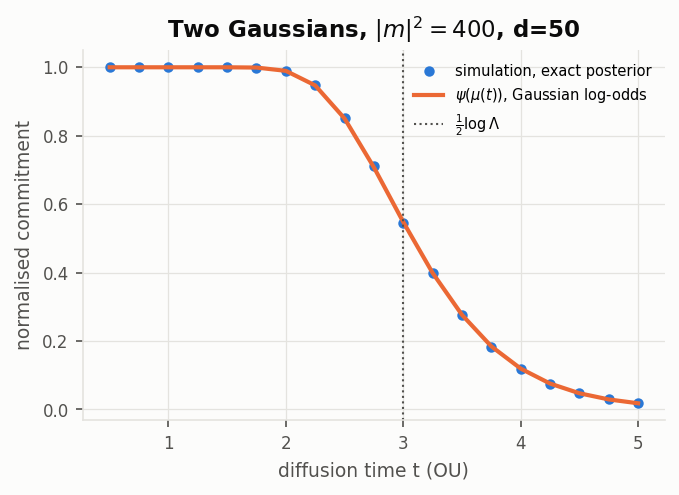
\includegraphics[width=0.32\textwidth]{tests/test_17_regimes/test_gaussian_mixture_speciation/gaussian_speciation.png}\hfill
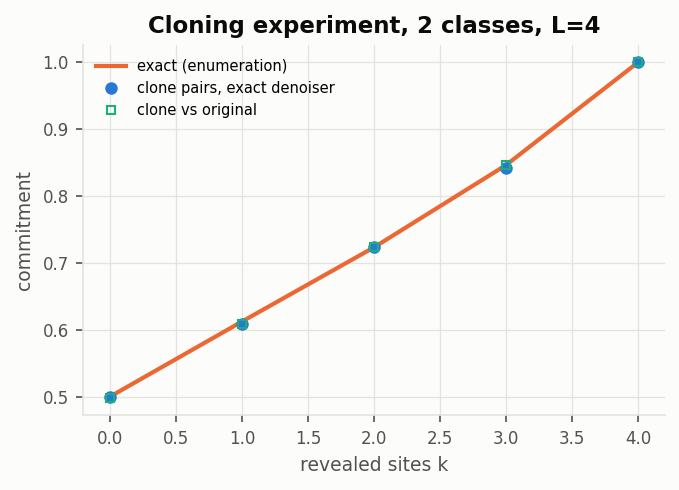
\includegraphics[width=0.32\textwidth]{tests/test_17_regimes/test_cloning_with_exact_denoiser_gives_exact_commitment/cloning_exact.png}\hfill
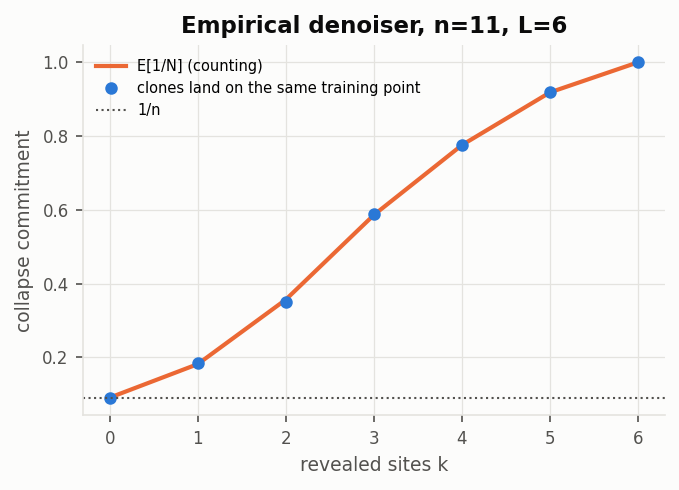
\includegraphics[width=0.32\textwidth]{tests/test_17_regimes/test_empirical_denoiser_collapse_is_one_over_n/empirical_collapse.png}
\caption{Tests of the measurement tools. Left: two Gaussian classes under OU noise; the commitment follows the
universal curve $\Psi(\mu_t)$ and crosses $1/2$ near $\frac12\log\Lambda_{\max}$. Middle: cloning with the exact denoiser
reproduces the exact commitment. Right: with the empirical denoiser, the probability that two clones land on the same
training sequence is $\E[1/N]$.}
\label{fig:dr_tests}
\end{figure}


%==========================================================================================
\section{Results}\label{sec:dr_results}
%==========================================================================================
Run:
\begin{center}\small\texttt{python scripts/s13\_dynamical\_regimes.py -{}-config configs/md\_unconditional.json}\end{center}
It took 37 minutes. The GPU throttled at 87\,°C, and the $4\times10^5$ clone completions account for 34 of those minutes. Outputs:
\begin{itemize}[nosep]
\item numbers: \texttt{evaluations/md\_unconditional/regimes.json};
\item figures: \texttt{figures/models/md\_unconditional/regimes/}.
\end{itemize}
With 1000 starting points, the standard error of each commitment value is $\le0.01$ (error bars in
Fig.~\ref{fig:dr_spec}).

\subsection{Speciation: a cascade, family first}
\begin{center}\footnotesize
\begin{tabular}{lccccc}
\toprule
 & sibling $D$ & Gaussian law \eqref{eq:ts_mask} & profile Bayes & \multicolumn{2}{c}{cloning with the network}\\
level & (nats) & $k_S$ ($t_S$) & $k_S$ ($t_S$) & (A) true $\bm x_t$: $k_S$ ($t_S$) & (B) own paths: $k_S$ ($t_S$)\\
\midrule
family & 64.5 & 1.6 (0.974) & 2.1 (0.960) & \textbf{2.0} (0.961) & 2.0 (0.962)\\
subfamily & 23.5 & 4.4 (0.927) & 4.9 (0.912) & \textbf{5.7} (0.899) & 5.6 (0.899)\\
clade & 10.4 & 9.8 (0.836) & 8.1 (0.859) & \textbf{16.0} (0.732) & 17.6 (0.700)\\
\bottomrule
\end{tabular}
\end{center}
$k_S$ is the number of revealed sites at which the normalised commitment $\psi$ crosses $1/2$. $t_S$ is the same
crossing for the curve averaged over the binomial number of revealed sites at masking time $t$, eq.~\eqref{eq:k_to_t}.

\begin{figure}[H]
\centering
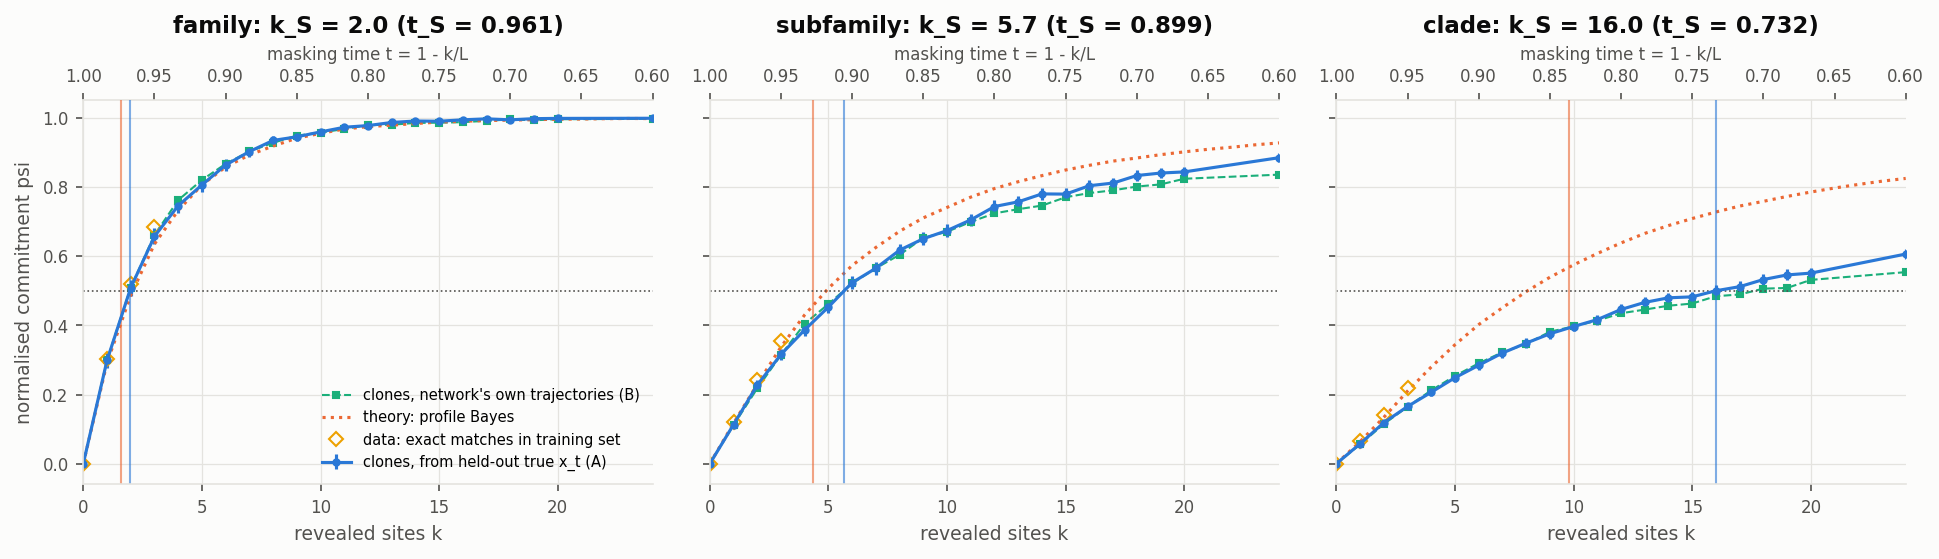
\includegraphics[width=\textwidth]{models/md_unconditional/regimes/speciation.png}
\caption{Speciation at the three levels of the tree. Blue: clone agreement from masked held-out true sequences (A).
Green, dashed: from the network's own trajectories (B). Orange, dotted: the profile-Bayes theory. Yellow diamonds:
the model-free estimate from exact matches in the training set, shown where $\ge90\%$ of the starting points have at
least 20 matches ($k\le3$). Vertical lines: the Gaussian law \eqref{eq:ts_mask} (orange) and the measured $k_S$ (blue).
Top axis: $t=1-k/L$.}
\label{fig:dr_spec}
\end{figure}

\paragraph{The hierarchy is decided top-down.} The family is decided after about \textbf{2 revealed sites}
($t_S=0.96$), the subfamily after about \textbf{6} ($t_S=0.90$), and the clade much later, after about \textbf{16}
($t_S=0.73$). The order follows the sibling divergences $D$, as \eqref{eq:ts_mask} predicts: the more two sibling
classes differ, the fewer residues are needed to tell them apart. The two starting ensembles give the same curves,
as they must for a model whose trajectories are consistent with its own samples (\S\ref{sec:dr_mask_spec}).

\paragraph{Family level: the network is exact.} The three independent estimates agree:
\begin{center}\footnotesize
\begin{tabular}{lccc}
\toprule
$\psi$ at $k=$ & 1 & 2 & 3\\
\midrule
data only (exact matches in the 144\,000 training sequences) & 0.30 & 0.52 & 0.68\\
network clones (A) & 0.30 & 0.51 & 0.66\\
profile Bayes & 0.29 & 0.49 & 0.64\\
\bottomrule
\end{tabular}
\end{center}
With 64.5 nats of class information spread over 60 sites, one revealed residue carries about 1 nat about the family.
Two residues take the commitment halfway, and by $k=10$ it is 0.96.

\paragraph{Subfamily and clade levels: the network commits too slowly.} Here the network's curves lie below both the
data and the theory. At $k=3$ the model-free estimate is 0.36 (subfamily) and 0.22 (clade); the network gives 0.32 and
0.17. Proposition~\ref{prop:clone}(ii) gives an independent check that needs no reference. With the exact denoiser,
two clones agree exactly as often as a clone agrees with the original sequence. For the network:
\begin{center}\footnotesize
\begin{tabular}{lcccccc}
\toprule
 & \multicolumn{2}{c}{family} & \multicolumn{2}{c}{subfamily} & \multicolumn{2}{c}{clade}\\
$k$ & clone--clone & clone--original & clone--clone & clone--original & clone--clone & clone--original\\
\midrule
2 & 0.672 & 0.668 & 0.315 & 0.313 & 0.168 & 0.173\\
5 & 0.871 & 0.879 & 0.515 & 0.529 & 0.290 & 0.317\\
10 & 0.973 & 0.977 & 0.711 & 0.741 & 0.430 & 0.479\\
20 & 0.999 & 0.999 & 0.861 & 0.890 & 0.576 & 0.646\\
\bottomrule
\end{tabular}
\end{center}
(``clone--original'' uses the true label of the original sequence.) At the family level the two columns agree, so
the network behaves like the exact denoiser. At the subfamily and clade levels, clones agree with the original more
than with each other. Write $Q(y\mid\bm x_U)$ for the network's class distribution of completions and $P$ for the
true one. Clone--clone is $\E\sum_yQ^2$ and clone--original is $\E\sum_yPQ$. The second exceeding the first means
that $Q$ is \emph{flatter} than $P$: the network spreads its completions over sibling subfamilies and clades too
evenly. This is the same weakness Part~III found from the other side: within-family correlations about 10\% too weak,
and per-clade $r_C=0.764$ against 0.828 for true samples. The fine-grained, clade-specific structure is learned
only partially, so the network decides the clade late.

\paragraph{Two caveats on the clade value.} (1) Clades genuinely overlap. Even the profile posterior of a
\emph{complete} sequence reaches only $\psi=0.94$, and the classifier that labels the clones is right for 91.5\% of
clades. The clade curve therefore rises slowly towards its ceiling, and its $1/2$-crossing is sensitive: small
changes in the curve move $k_S$ by several sites. (2) The data-only estimate stops at $k=3$, because beyond that most
partial sequences have fewer than 20 exact matches. It is exact where it exists, so the robust statement is: at the
clade level the network is less committed than the data at every $k$ we can check, and its $k_S=16$ is an upper
bound on the true clade speciation. The profile theory places the true value near 8--10.

\begin{figure}[H]
\centering
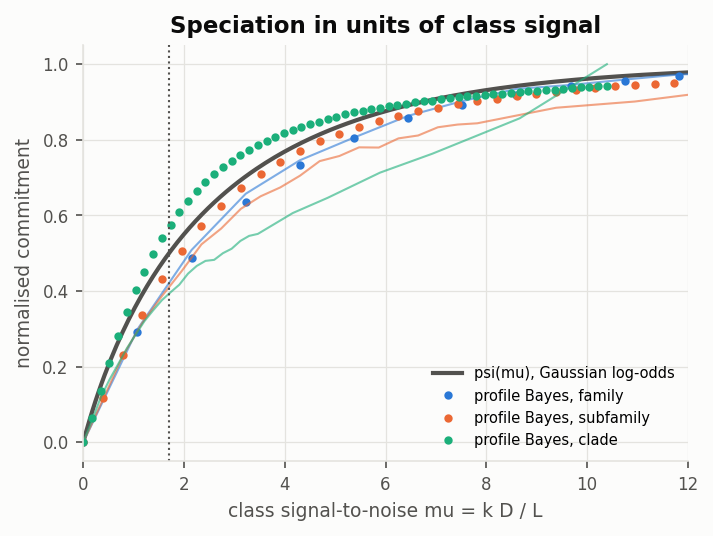
\includegraphics[width=0.46\textwidth]{models/md_unconditional/regimes/speciation_universal.png}\hfill
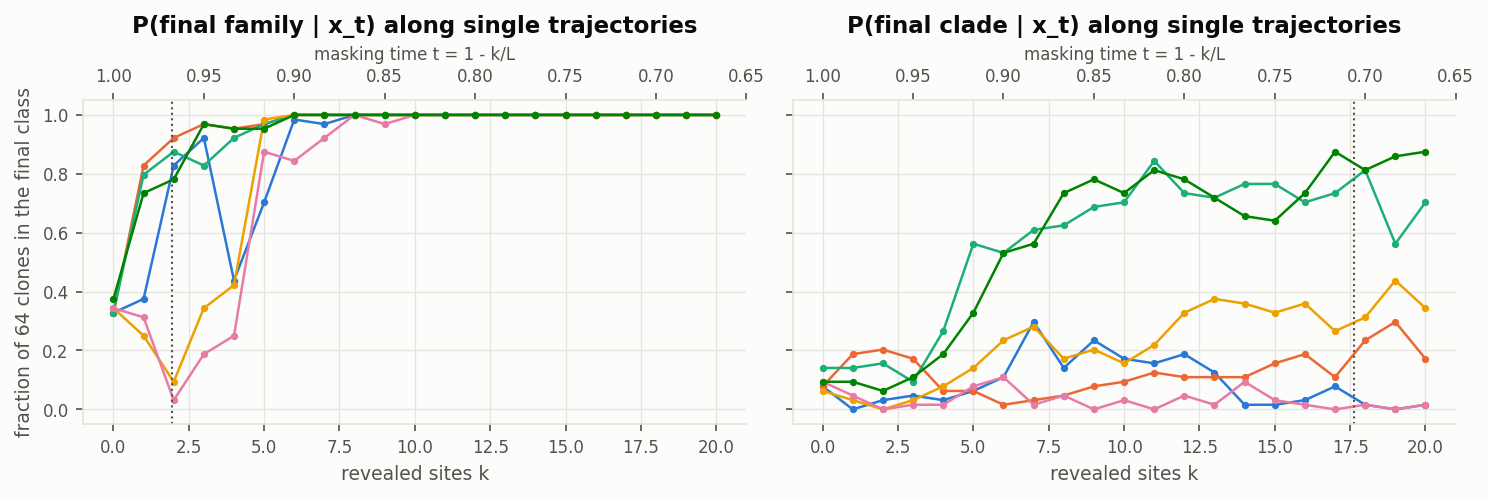
\includegraphics[width=0.52\textwidth]{models/md_unconditional/regimes/trajectories.png}
\caption{Left: the three levels in units of class signal-to-noise $\mu=kD/L$. Dots: profile Bayes. Thin lines:
network clones. Grey: the universal Gaussian curve $\Psi(\mu)$ \eqref{eq:psi_universal}. Right: six single trajectories
of the network, showing at each $k$ the fraction of 64 clones that end in the trajectory's final family (left panel)
or clade (right panel).}
\label{fig:dr_universal}
\end{figure}

\paragraph{One curve for all levels.} Rescaling $k$ by $D/L$ brings the three profile curves close to the single
curve $\Psi(\mu)$ (Fig.~\ref{fig:dr_universal}, left), as the Gaussian argument predicts. The remaining deviations
are expected. At small $\mu$, only a few sites are revealed and $\Lambda$ is a sum of a few non-Gaussian terms. At
large $\mu$ the clades overlap and never fully commit. The network's subfamily and clade curves fall below the
profile ones, which is the under-confidence above.

\paragraph{Single trajectories: symmetry breaking.} Fig.~\ref{fig:dr_universal} (right) is the masked analogue of the
paper's picture of a trajectory falling into one well. The family probability starts at 1/3 and jumps within the
first 2--5 revealed sites. Sometimes it first moves \emph{away} from the final family: the first residues can point
the wrong way, and the next ones correct it. After $k\approx6$ every trajectory is committed. The clade probability
starts at 1/18 and drifts slowly. Two of the six trajectories are clearly committed by $k=10$; the others are still
spread over several clades at $k=20$.

\subsection{Collapse: the quenched theory is exact, the annealed one is not}
\begin{center}\footnotesize
\begin{tabular}{lcc}
\toprule
collapse of the empirical denoiser, $n=144\,000$ & $k_C$ & $t_C$\\
\midrule
measured: $\E[1/N]$ on 1000 trajectories planted on training sequences & \textbf{6.2} & \textbf{0.891}\\
quenched theory \eqref{eq:collapse_mask}, $P(\bm x_U)$ from the network's chain rule & 6.4 & 0.889\\
entropy criterion $H(k_C)=\log n=11.88$ & 6.5 & --\\
annealed theory (collision probability \eqref{eq:collision}) & 10.4 & 0.825\\
\bottomrule
\end{tabular}
\end{center}
\begin{figure}[H]
\centering
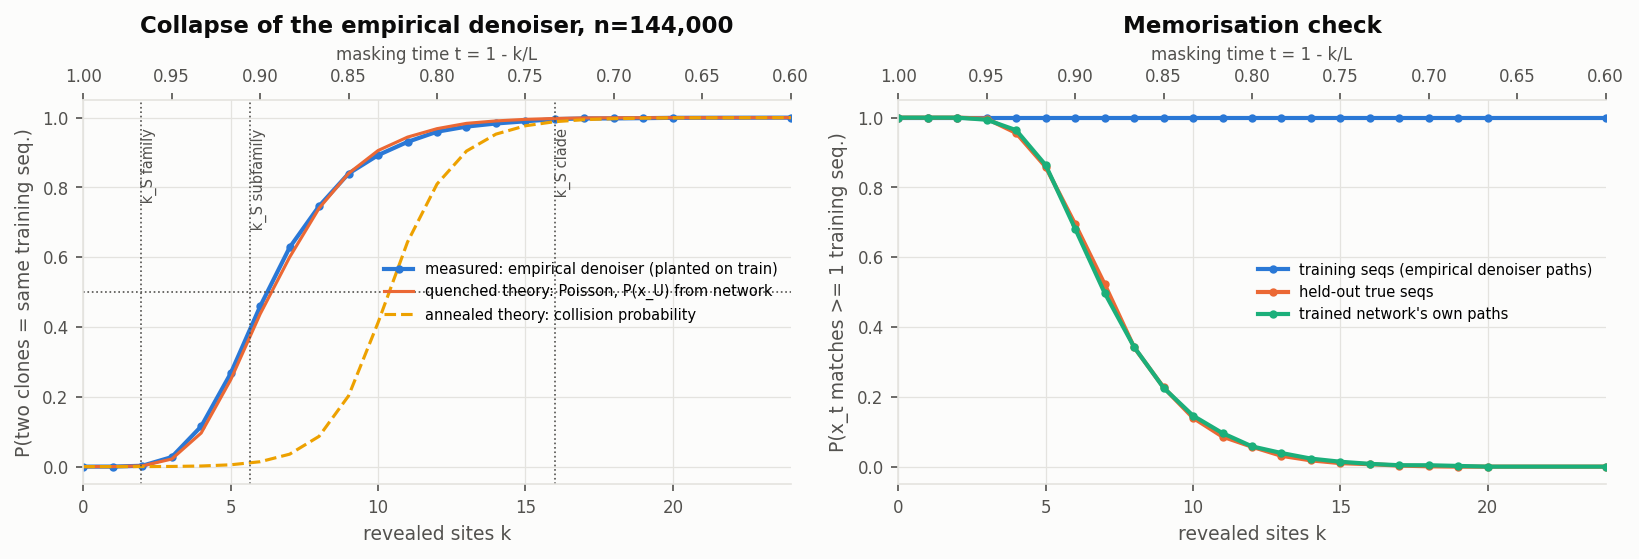
\includegraphics[width=\textwidth]{models/md_unconditional/regimes/collapse.png}
\caption{Left: probability that two clones of the empirical denoiser end on the same training sequence (blue). The
quenched Poisson prediction (orange) follows it at every $k$; the annealed prediction (yellow, dashed) is 4 sites
late. Dotted verticals: the network's speciation times. Right: probability that $\bm x_t$ still agrees with at least one
training sequence, for trajectories planted on training sequences (the empirical denoiser's), held-out true sequences,
and the trained network's own trajectories.}
\label{fig:dr_coll}
\end{figure}
The quenched formula has no fitted parameter. It uses only the network's probabilities of the revealed residues, and
it reproduces the measured collapse curve at every $k$ (Fig.~\ref{fig:dr_coll}, left). The annealed version collapses
4 sites too late. The collision probability is dominated by rare close pairs of training sequences: its entropy
$H_2(k)$ is well below $H(k)$ (Fig.~\ref{fig:dr_entropy}), so it predicts far more matches than a typical trajectory
sees. This is the Random-Energy-Model lesson of \S\ref{sec:dr_gauss_coll} in a setting where it can be checked
exactly.

\paragraph{Collapse versus the number of training sequences.} Measured on random training subsets, and predicted with
the same formula:
\begin{center}\footnotesize
\begin{tabular}{lcccc}
\toprule
$n$ & 100 & 1\,000 & 10\,000 & 144\,000\\
\midrule
$k_C$ measured & 2.12 & 3.38 & 4.70 & 6.43\\
$k_C$ quenched theory & 2.11 & 3.40 & 4.74 & 6.39\\
\bottomrule
\end{tabular}
\end{center}
(The last column repeats the measurement with a different random set of planted sequences: 6.43 against 6.24 above.
This is the size of the sampling noise.)

\begin{figure}[H]
\centering
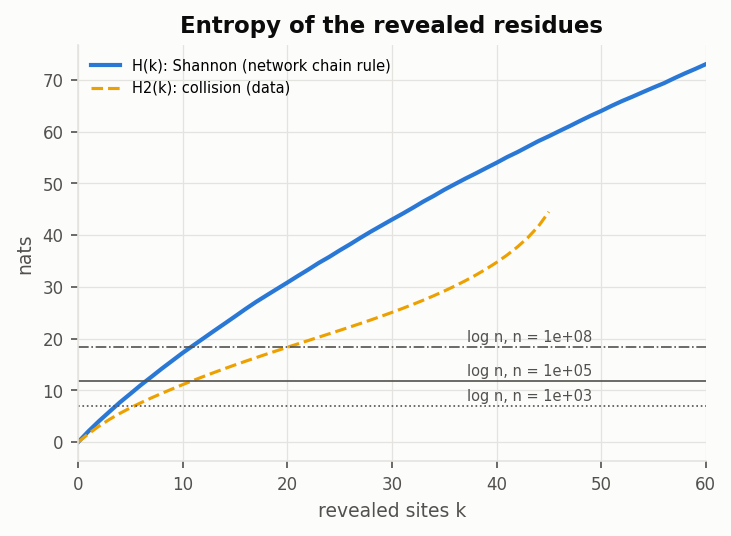
\includegraphics[width=0.46\textwidth]{models/md_unconditional/regimes/entropy.png}\hfill
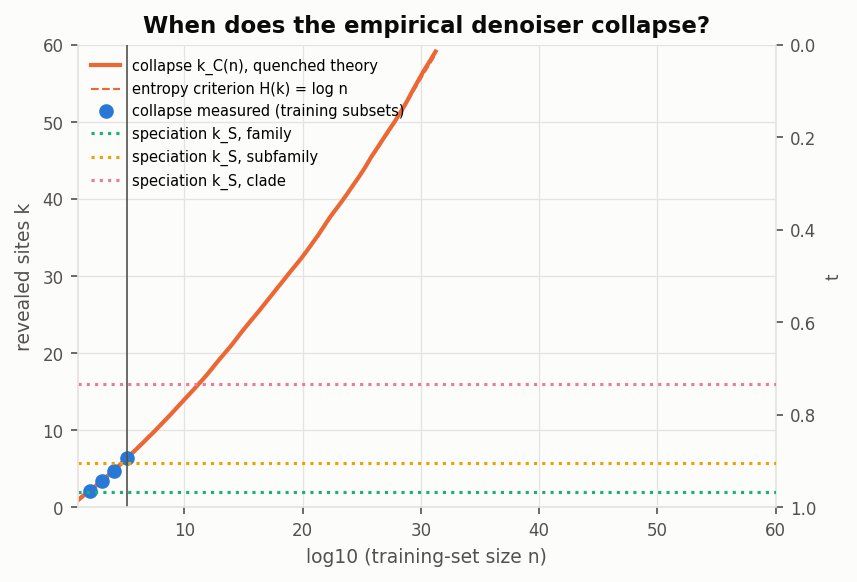
\includegraphics[width=0.5\textwidth]{models/md_unconditional/regimes/phase_diagram.png}
\caption{Left: entropy of the revealed residues. $H(k)$ comes from the network's chain rule; it is 2.1 nats for the
first site and reaches 73.0 nats (1.22 per site, the NELBO) at $k=60$. $H_2(k)$ comes from pairwise Hamming distances. The
collapse happens where $H(k)$ crosses $\log n$. Right: the phase diagram. Collapse $k_C(n)$ (theory line, measured
points) against the three speciation levels. The vertical line marks our $n$.}
\label{fig:dr_entropy}
\end{figure}

\subsection{The three regimes for our data}
For $n=144\,000$, the times of the backward process in order of occurrence are:
\[
\underbrace{k_S^{\rm family}\approx2}_{t=0.96}\;<\;\underbrace{k_S^{\rm subfamily}\approx6}_{t=0.90}\;\lesssim\;
\underbrace{k_C\approx6}_{t=0.89}\;<\;\underbrace{k_S^{\rm clade}\approx8\text{--}16}_{t=0.86\text{--}0.73}.
\]
So the \emph{empirical} denoiser decides the family and, barely, the subfamily before collapsing onto a training
sequence. The clade is never ``speciated'' by it: it is inherited from the memorised sequence. Regimes I, II and III
are cleanly separated only at the family level. The training-set size needed to separate them at level $\ell$ is
$n^\star_\ell=e^{H(k_S^\ell)}$:
\begin{center}\footnotesize
\begin{tabular}{lccc}
\toprule
 & family & subfamily & clade\\
\midrule
$n^\star$ (with the network's $k_S$) & 54 & $3.5\times10^4$ & $1.5\times10^{11}$\\
$n^\star$ (with the profile-Bayes $k_S$) & 68 & $1.0\times10^4$ & $1.6\times10^6$\\
\bottomrule
\end{tabular}
\end{center}
The reason is the entropy scale. One residue carries about 2 nats, so $\log n$ is used up after $\approx6$ residues,
while telling two sibling clades apart takes 8--16. In the paper's language, $\alpha=\log n/L=0.20$ nats per site
is small compared with the entropy per site (1.22 nats). This is the data-poor regime, where the exact minimiser of the
loss memorises early.

\subsection{The trained network does not memorise}
The trained network has the same loss as the empirical denoiser, so the question is how close it gets to that
minimiser. The answer is: not close.
\begin{itemize}[nosep]
\item Along its own trajectories, the probability that $\bm x_t$ still matches a training sequence falls exactly as it
does for \emph{held-out} true sequences (0.50 vs 0.52 at $k=7$, 0.15 vs 0.14 at $k=10$, zero after $k\approx20$). Along
the empirical denoiser's trajectories it stays at 1 (Fig.~\ref{fig:dr_coll}, right). The mean number of matches also
agrees with the held-out value at every $k$ (e.g.\ 24.0 vs 24.6 at $k=7$).
\item Its NELBO is 1.187 nats per site on training sequences and 1.219 on test sequences. That is a gap of 0.03,
against 0.198 (train) and $+\infty$ (test) for the empirical denoiser. The chain-rule entropy of training sequences is
71.5 nats against 73.0 for test sequences. There is a small beginning of preference for training data, far from
memorisation.
\end{itemize}
In the three-regime picture, the network's trajectories pass through regimes I and II and end in regime II. They
never enter regime III. The network generalises although its loss's exact minimiser would collapse after 6 residues.
Generalisation comes from what the network can represent easily and from finite training, not from reaching the
optimum of its loss. (The paper makes the same point for Gaussian diffusion: networks memorise when $n$ is small
compared with their capacity or when they are trained for very long.)

\begin{keybox}{Summary of Part IV}
\begin{itemize}[nosep,leftmargin=*]
\item The two times of Biroli, Bonnaire, de Bortoli and Mézard transpose to masked diffusion with exact
statements. Speciation is the collision probability of the class posterior, measured by cloning. It follows a
universal curve in the class signal-to-noise ratio $\mu$, which for masking is $\mu=(1-t)D$ (for Gaussian noise,
$2\Lambda_{\max}e^{-2t}$). Collapse is $\E[1/N]$, with $N-1$ Poisson-distributed; it happens when the entropy of the
revealed residues reaches $\log n$.
\item Speciation is hierarchical. Family after $\approx2$ residues ($t_S=0.96$), subfamily after $\approx6$ (0.90),
clade after 8--16 (0.86--0.73). At the family level, the network, the data and the theory agree within 0.02.
\item At the subfamily and clade levels the network commits too slowly: its completions are spread too evenly over
sibling classes. This was detected without any reference, by comparing clone--clone with clone--original agreement.
\item The empirical denoiser (the exact optimum of the loss) collapses after 6.2 residues ($t_C=0.89$), between
subfamily and clade speciation. The quenched Poisson theory predicts this to within 0.2 sites for $n$ from $10^2$ to
$1.4\times10^5$; the annealed one is 4 sites late.
\item The trained network does not collapse. Its trajectories leave the training set exactly like held-out data, and its
train/test likelihood gap is 0.03 nats per site.
\end{itemize}
\end{keybox}


\part{Code and reproduction}

%==========================================================================================
\section{Code, tests and folder layout}
%==========================================================================================
\subsection{Folder layout}
{\small\begin{verbatim}
protein_seq_gen/
  configs/ground_truth.json      all parameters of this document
  src/psg/                       the library
     alphabet.py   encoding, FASTA I/O
     potts.py      Potts class: energy, local field, conditional, zero-sum gauge
     hierarchy.py  contact map, tree, distances, distance theory
     sampling.py   Gibbs sampler (numpy)   torch_sampling.py  Gibbs sampler (GPU)
     stats.py      f_i, f_ij, C_ij, compare_statistics, identity, PCA
     data.py       top-up, train/val/test split, tags
     models/factored_attention.py   the two transformers (Part II)
     training.py   PL training loop        evaluation.py  J recovery, contacts
     distances.py  Hamming, nearest neighbour, Wasserstein, Frechet distance
     models/masked_diffusion.py  denoiser, NELBO, samplers (III)
     diffusion_training.py       training loop, EMA, checkpoints
     regimes.py                  speciation / collapse tools (IV)
     plots.py      all figures (one visual style)
  scripts/                       s01..s03 (Part I), s04 dataset, s05 train, s06 evaluate,
                                 s07 J vs tree, s08 mode mixing,
                                 s09/s10 train/evaluate diffusion,
                                 s11 compare models, s12 t-dependence,
                                 s13 dynamical regimes
  tests/                         test_01 ... test_17 (pytest)
  data/ground_truth_potts/       31 models (.npz), contact_map.npy, tree.json
  data/sequences/                FASTA per clade + all_sequences.npz (labels)
  data/splits/                   train/val/test.npz, test_fasta/ (held out)
  evaluations/ground_truth/      JSON reports, PCA reference, frequencies, energy traces
  figures/ground_truth/          01_hierarchy, 02_sampling, 03_analysis
  figures/models/<run>/          training curve, PCA, r_C per clade
  figures/tests/<test>/<case>/   outcome plots of each test
  models/<run>/ sampling/<run>/  trained models / their generated sequences
  docs/                          this document
\end{verbatim}}

\subsection{What each test checks (Part I; Part II in \S\ref{sec:p2tests})}
\begin{center}
\small
\begin{tabular}{p{0.3\linewidth}p{0.62\linewidth}}
\toprule
test & what it verifies\\
\midrule
\texttt{test\_01\_potts} & energy of an $L=2,q=2$ model by hand; exact probabilities; conditionals $=$ ratios of enumerated probabilities; neighbour-restricted field; gauge keeps $P$ and is a projection; save/load; FASTA round-trip\\
\texttt{test\_02\_sampling} & $J=0$ marginals $=$ softmax$(h)$; $L=3,q=3$ Gibbs vs.\ exact (TV $<0.02$); energy relaxes and plateaus\\
\texttt{test\_03\_hierarchy} & tree shape; symmetry, zero-sum, couplings only on contacts; strict hierarchical ordering of distances; distances match eqs.\ \eqref{eq:dJ}--\eqref{eq:dh} within $10\%$; reproducible with a seed\\
\texttt{test\_04\_stats} & $f_i,f_{ij},C_{ij}$ on a 4-sequence alignment by hand; copied column gives $C=\mathrm{diag}(f)-ff^\top$; independent columns give $C\approx0$; metric $=1$ on identical sets and $\approx0$ on column-shuffled sets; PCA splits two clusters perfectly\\
\texttt{test\_05\_pipeline} & the three scripts end-to-end on a tiny tree; the sequence statistics come out in hierarchical order\\
\texttt{test\_06} \dots\ \texttt{test\_17} & Parts II--IV, see \S\ref{sec:p2tests}, \S\ref{sec:md_tests}, \S\ref{sec:dr_tests}\\
\bottomrule
\end{tabular}
\end{center}
Run everything with \texttt{python -m pytest} (76 tests). Reproduce everything with the scripts s01--s13
in order.

\end{document}
